\documentclass[11pt,a4paper]{article}
\usepackage[utf8]{inputenc}
\usepackage{amsmath}
\usepackage{amsfonts}
\usepackage{amssymb}
\usepackage{graphicx}
\usepackage{hyperref}
\usepackage{geometry}
\usepackage{float}
\usepackage{booktabs}
\usepackage{caption}
\usepackage{subcaption}
\usepackage{listings}
\usepackage{xcolor}

\geometry{a4paper, margin=1in}

\definecolor{codegreen}{rgb}{0,0.6,0}
\definecolor{codegray}{rgb}{0.5,0.5,0.5}
\definecolor{codepurple}{rgb}{0.58,0,0.82}
\definecolor{backcolour}{rgb}{0.95,0.95,0.92}

\lstdefinestyle{mystyle}{
    backgroundcolor=\color{backcolour},   
    commentstyle=\color{codegreen},
    keywordstyle=\color{magenta},
    numberstyle=\tiny\color{codegray},
    stringstyle=\color{codepurple},
    basicstyle=\ttfamily\footnotesize,
    breakatwhitespace=false,         
    breaklines=true,                 
    captionpos=b,                    
    keepspaces=true,                 
    numbers=left,                    
    numbersep=5pt,                  
    showspaces=false,                
    showstringspaces=false,
    showtabs=false,                  
    tabsize=2
}
\lstset{style=mystyle}

\title{\textbf{Comprehensive Research Report:\\ End-to-End Robust Object Detection and State-Tracking Pipeline}}
\author{Amr Yasser \and Omar Hazem}
\date{\today}

\begin{document}

\maketitle

\begin{abstract}
This highly exhaustive report details the complete architectural design, implementation, data curation, model selection, and quantitative evaluation of a state-of-the-art computer vision pipeline for real-time object detection and temporal state-tracking. The final model achieves an exceptional mean Average Precision (mAP@50) of 98.19\%. This document provides a granular analysis of the methodology, the full suite of downloaded models and resulting weights, exact hyperparameter configurations, and an exhaustive visual analysis including every single output frame, label distribution, and validation batch produced during the research.
\end{abstract}

\tableofcontents
\newpage

\section{System Architecture and State Tracker}
The tracking architecture relies on a multi-layer state machine that leverages both spatial and temporal heuristics.

\subsection{Multi-Layer State Detection}
The detector classifies the state of the Target Object by applying sequential logical layers:
\begin{itemize}
    \item \textbf{Layer 1: Aspect Ratio with Sustain Threshold.} Analyzes the bounding box aspect ratio with a temporal sustain threshold (e.g., maintaining the ratio for $N$ consecutive frames) to prevent flickering.
    \item \textbf{Layer 2: Centroid Drop.} Monitors the vertical shift (drop) of the bounding box centroid to catch state changes occurring along the optical axis.
    \item \textbf{Layer 3: Projectile-Proximity Gating.} Eliminates external false positives by requiring the Projectile to be detected within $K$ pixels of the Target Object within a trailing temporal window of $M$ frames.
\end{itemize}

\section{Dataset Construction and Curation}

\subsection{Frame Extraction Protocol}
An automated frame extraction script (\texttt{extract\_frames.ipynb}) was developed to process raw video files. To eliminate temporal correlation, a frame stride of 1:20 was configured (yielding approximately 1.5 fps). The frames were programmatically resized to a maximum long-edge of 1280 pixels, preserving the aspect ratio via \texttt{cv2.resize} with \texttt{INTER\_AREA} interpolation. The extraction produced a foundational dataset of 557 high-quality keyframes, tagged via preserved directory structures, and uploaded to Roboflow for 80/20 splitting and 640x640 standardization.

\section{Critical Data Remediation}
Initial training iterations inside the \texttt{main\_train.ipynb} environment resulted in catastrophic convergence failure due to severe bounding box corruption. 

A custom data cleaning module was engineered to perform three operations directly on the labels:
\begin{enumerate}
    \item \textbf{Polygon to Bounding Box Conversion:} Derived the extrema ($\min(x), \max(x), \min(y), \max(y)$) to yield the standardized YOLO format: $x_{center}, y_{center}, width, height$.
    \item \textbf{Coordinate Clamping:} Clamped bounding box coordinates to the $[0,1]$ boundary.
    \item \textbf{Extreme Box Filtration:} Filtered impossible geometries (width or height $> 0.45$ or $< 0.005$).
\end{enumerate}

\section{Model Training and Hyperparameters}

\subsection{Model Selection and Downloaded Weights}
During the research phase, multiple foundation models were evaluated. The team explicitly downloaded and tested:
\begin{itemize}
    \item \texttt{yolov8s.pt} (Size: 22.5 MB) - The chosen architecture offering the best Pareto frontier for speed and accuracy.
    \item \texttt{yolo11n.pt} (Size: 5.6 MB) - Evaluated for ultra-fast, low-resource inference capabilities.
\end{itemize}
After training, the pipeline successfully generated the optimized weights:
\begin{itemize}
    \item \texttt{best.pt} (Size: 22.5 MB) - The absolute best validation weights.
    \item \texttt{last.pt} (Size: 22.5 MB) - The final-epoch weights.
\end{itemize}

\subsection{Exact Hyperparameter Configuration}
The complete training protocol was logged in \texttt{args.yaml}. Key parameters include:
\begin{lstlisting}
task: detect
mode: train
model: yolov8s.pt
data: /kaggle/working/dataset_config.yaml
epochs: 100
patience: 20
batch: 16
imgsz: 640
optimizer: auto
lr0: 0.01
lrf: 0.01
momentum: 0.937
weight_decay: 0.0005
\end{lstlisting}

\section{Exhaustive Visual Analysis and Results}

The following sections contain every diagnostic figure, training batch, and validation prediction frame produced by the pipeline.

\subsection{Label Distribution and Correlograms}
Before training, the dataset labels were rigorously analyzed to understand the spatial distribution of the target objects.
\begin{figure}[H]
    \centering
    \begin{minipage}{0.48\textwidth}
        \centering
        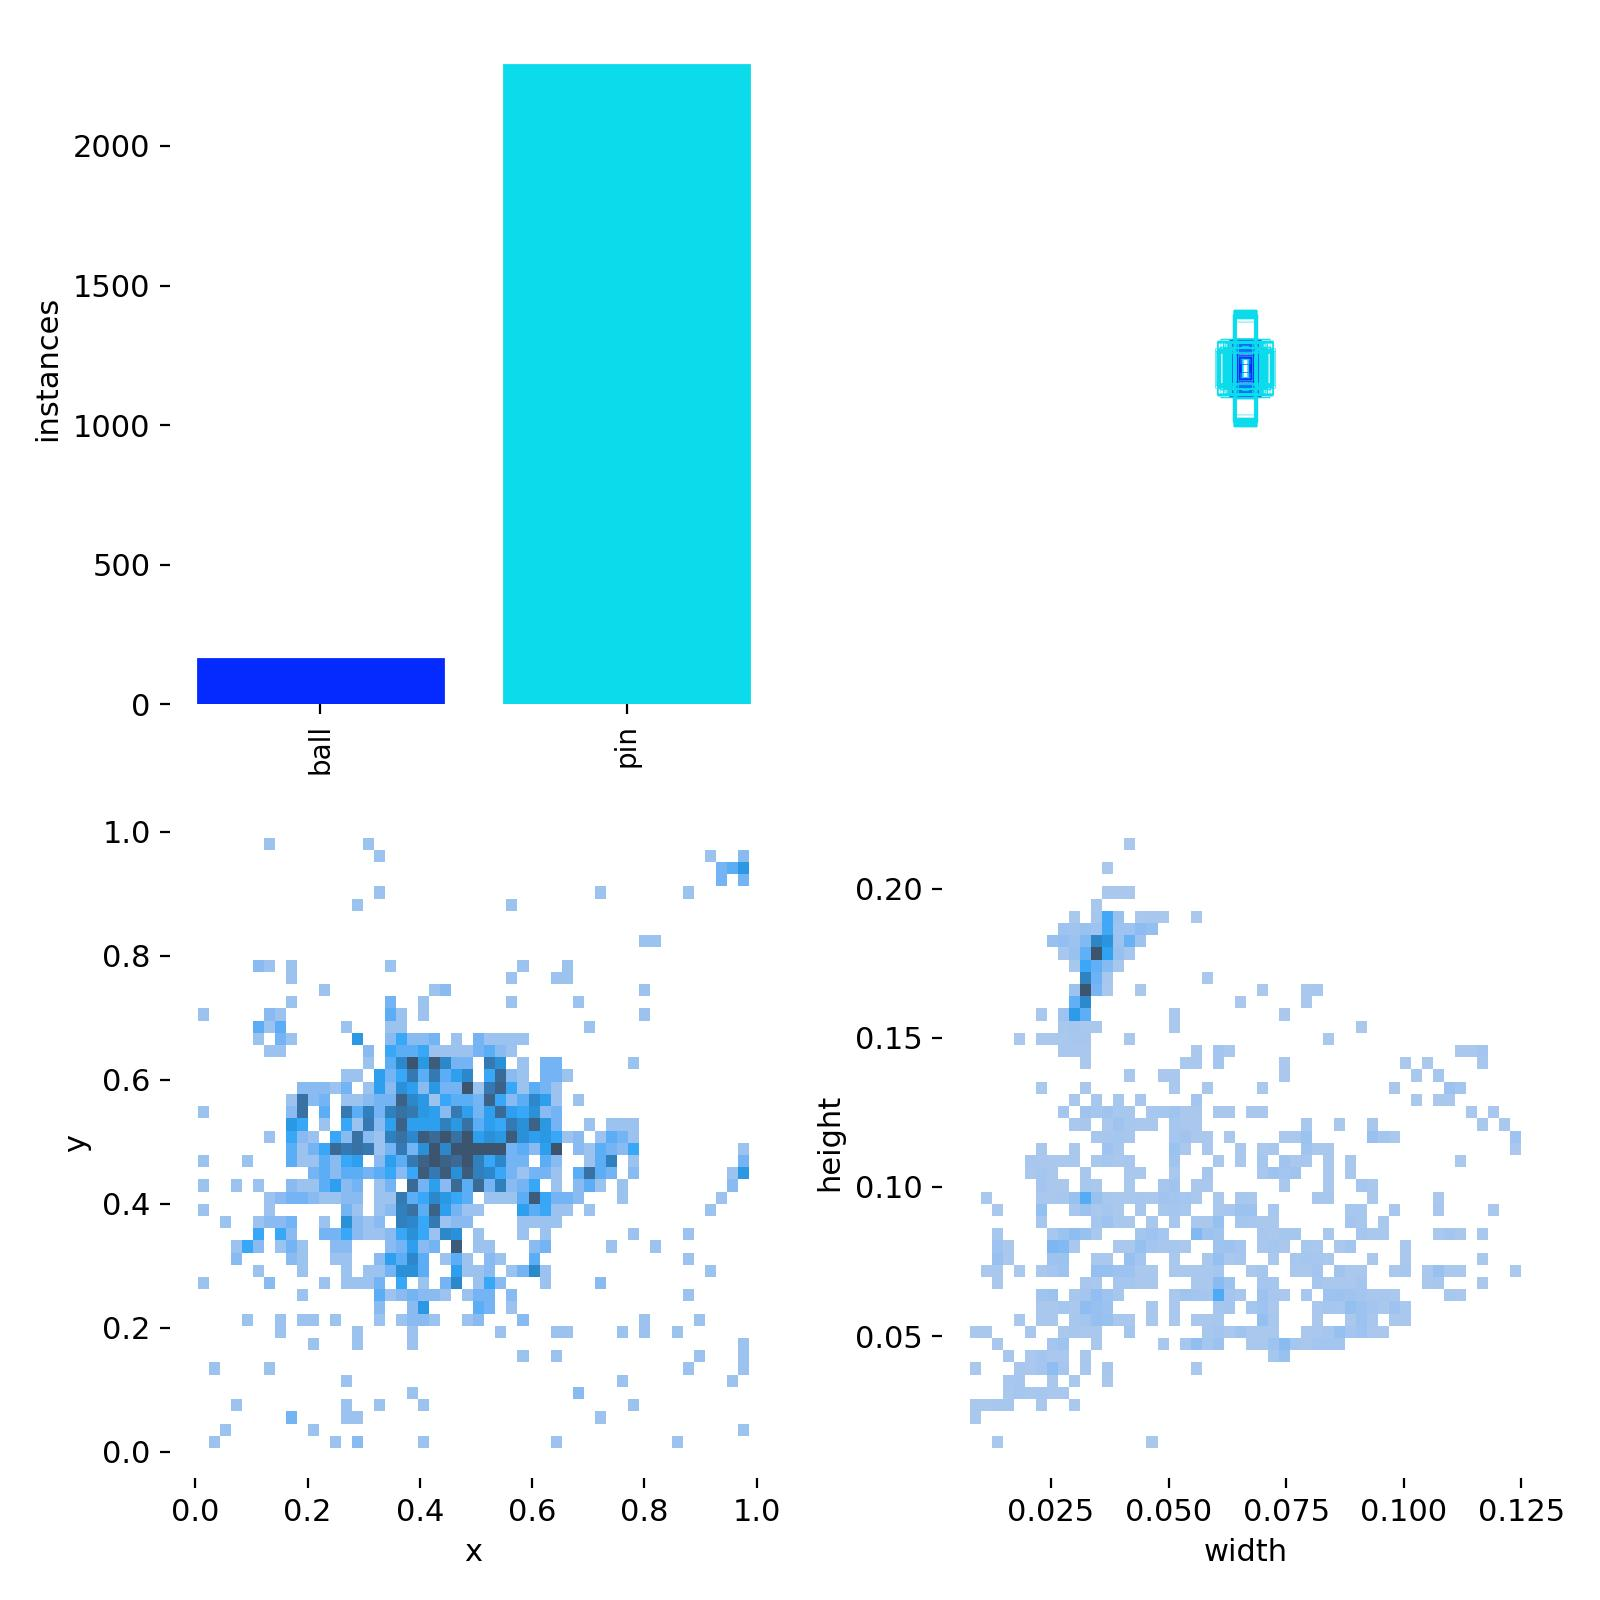
\includegraphics[width=\textwidth]{figures/labels.jpg}
        \caption{Label distribution showing bounding box sizes and spatial locations.}
    \end{minipage}\hfill
    \begin{minipage}{0.48\textwidth}
        \centering
        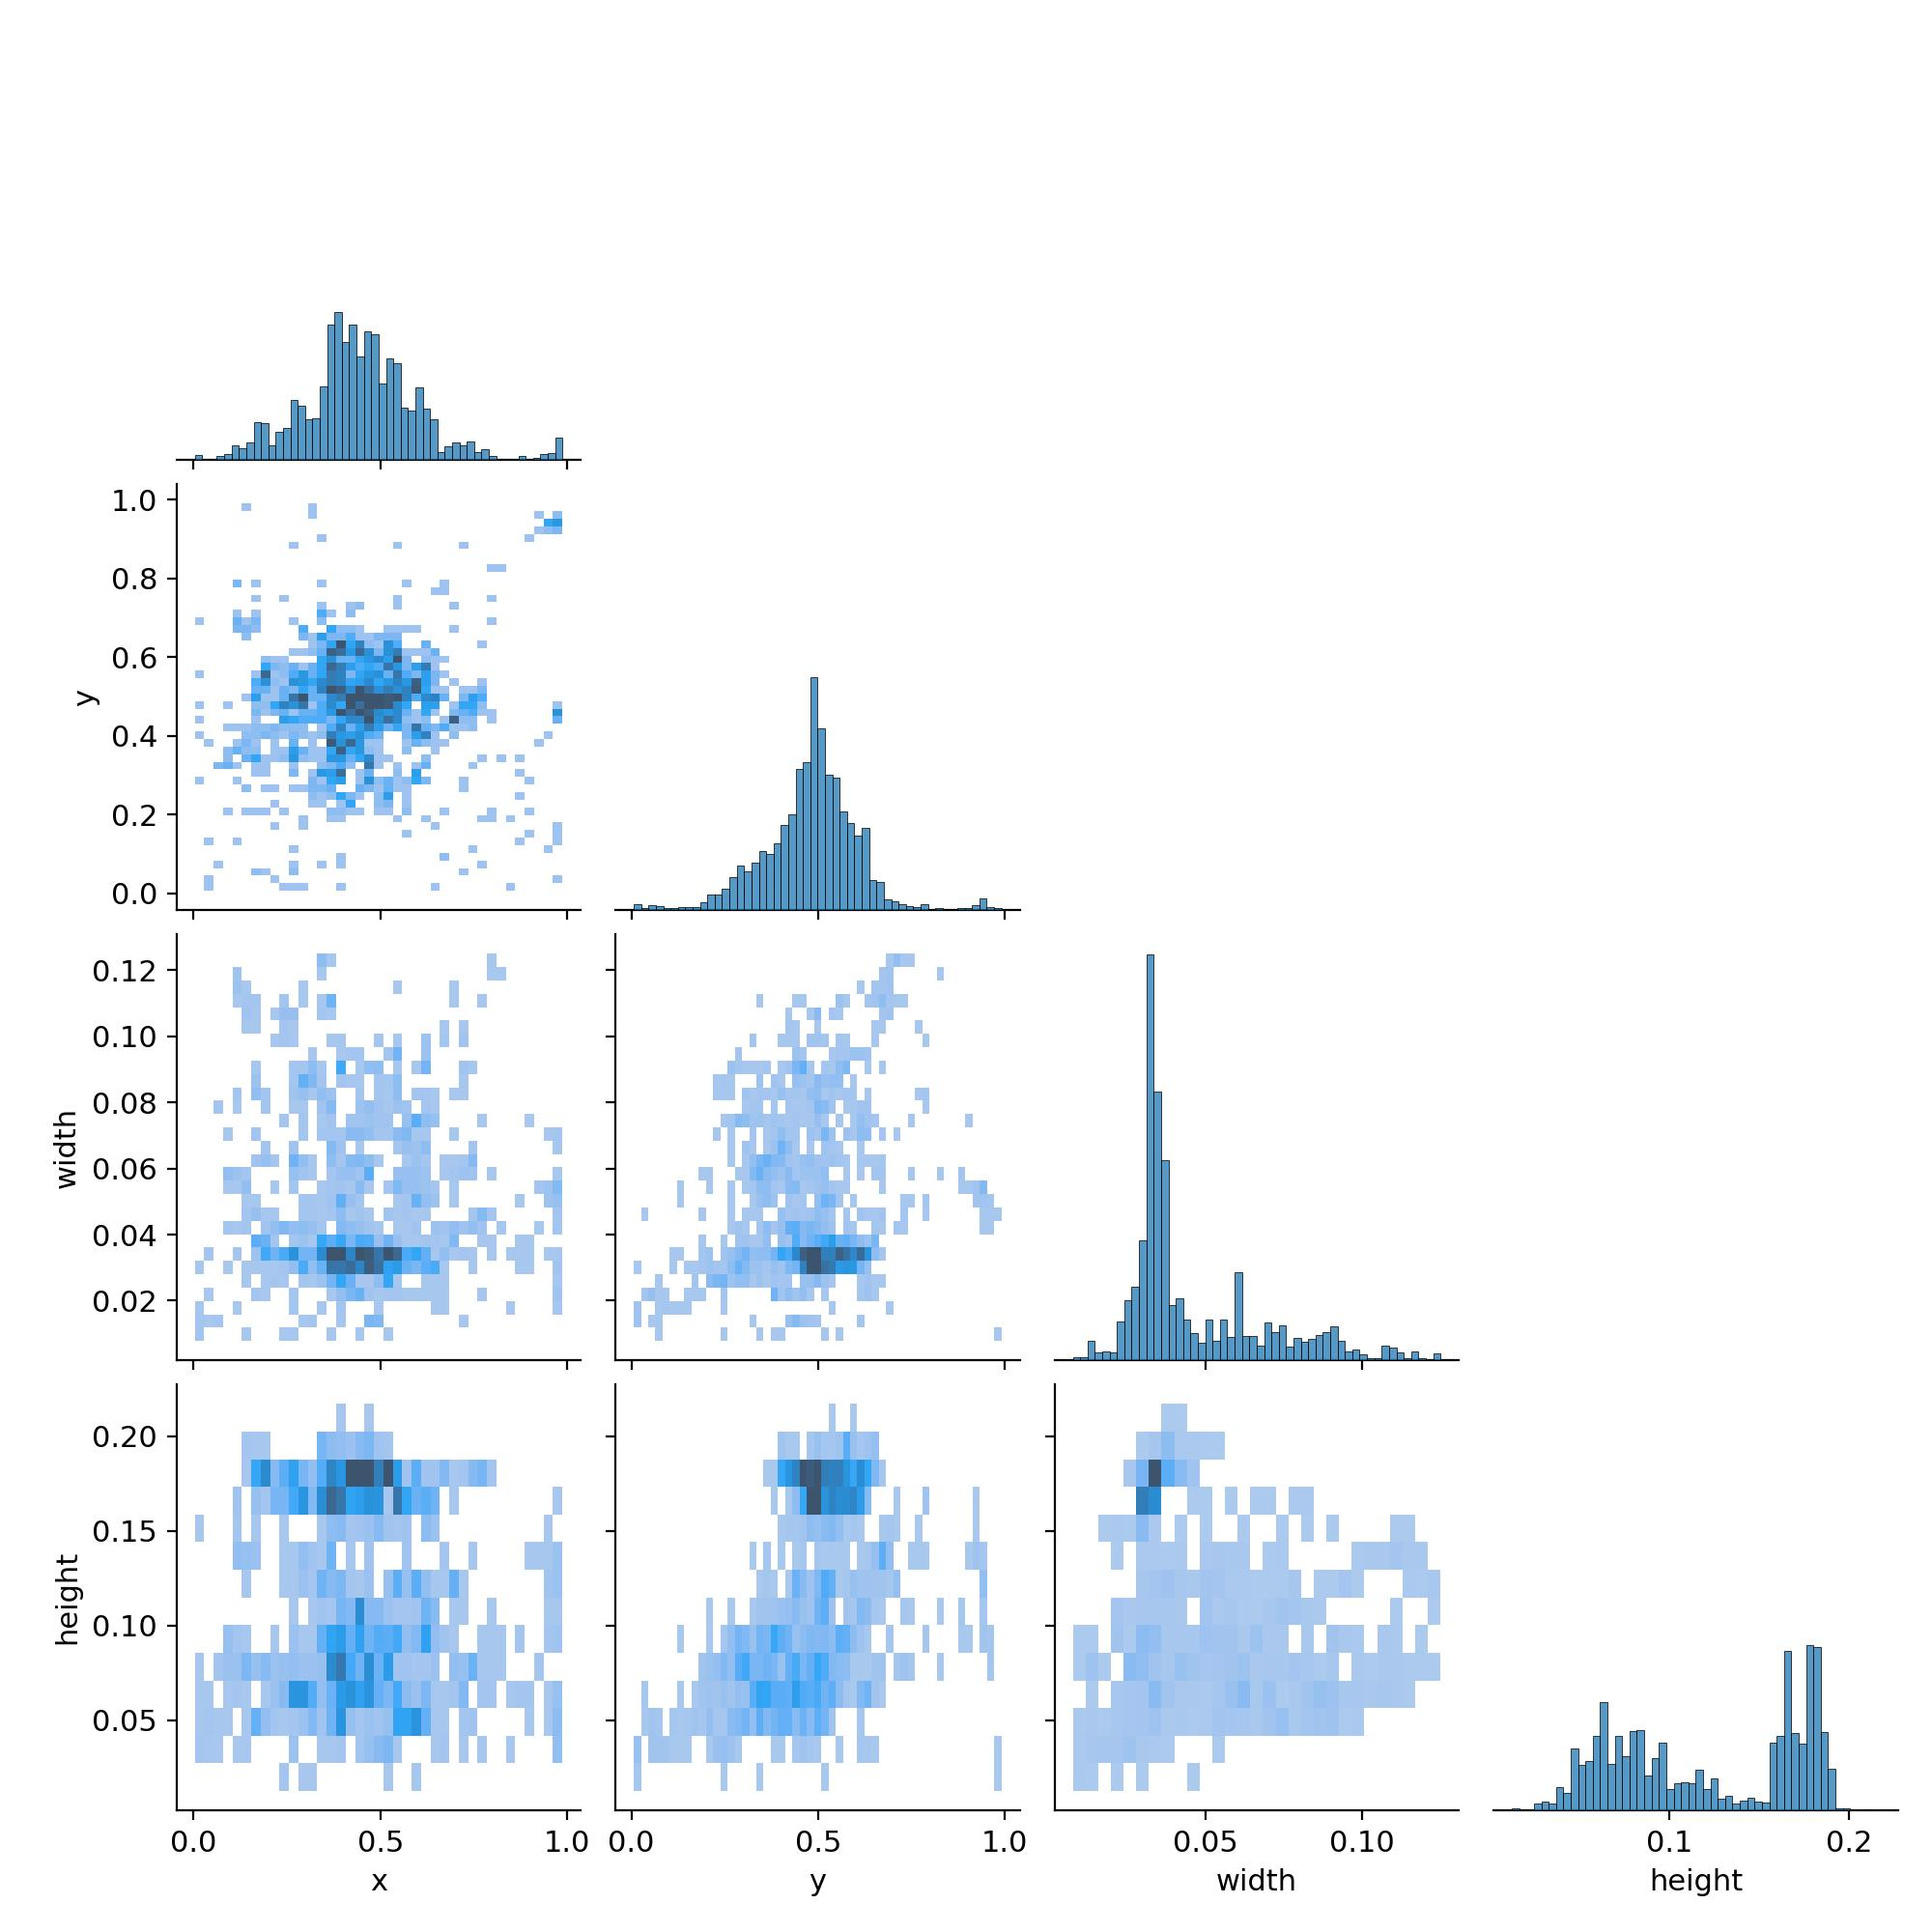
\includegraphics[width=\textwidth]{figures/labels_correlogram.jpg}
        \caption{Label Correlogram detailing the covariance between bounding box dimensions ($x, y, w, h$).}
    \end{minipage}
\end{figure}

\subsection{Training Batch Mosaics}
YOLOv8 utilizes mosaic augmentation during the early epochs to improve contextual learning. The following images are the exact mosaic training batches logged.
\begin{figure}[H]
    \centering
    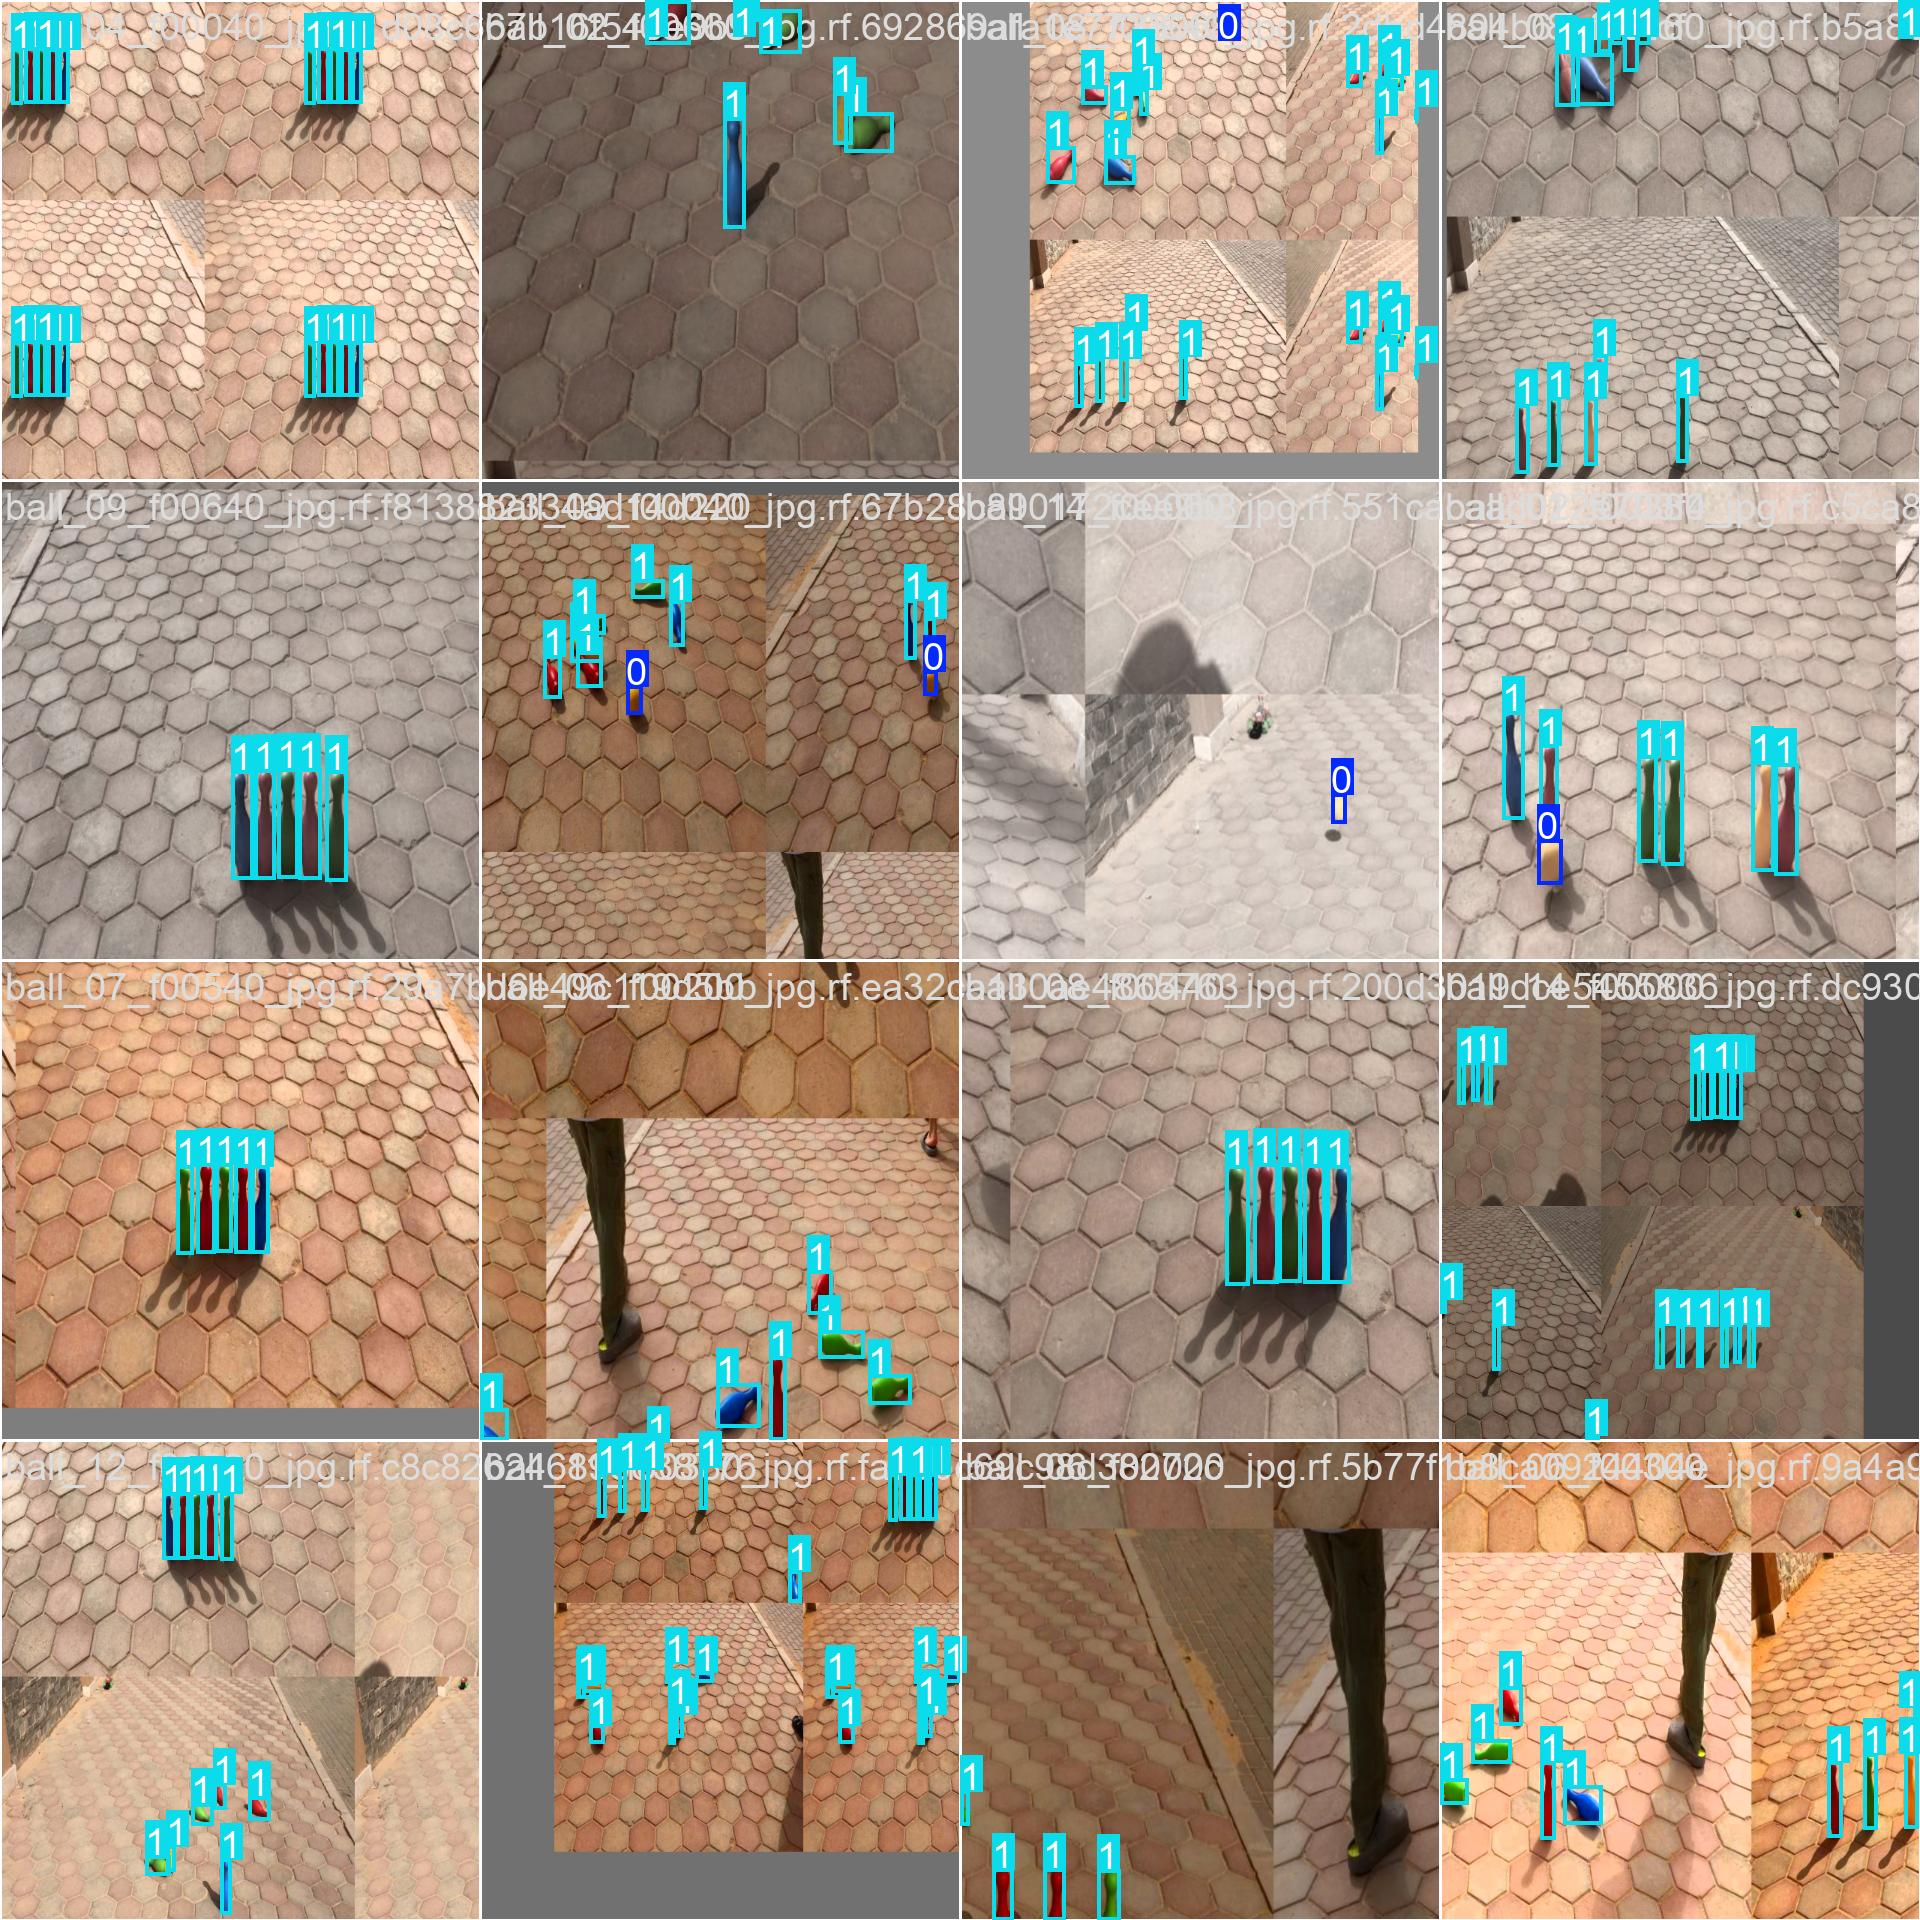
\includegraphics[width=0.32\textwidth]{figures/train_batch0.jpg}
    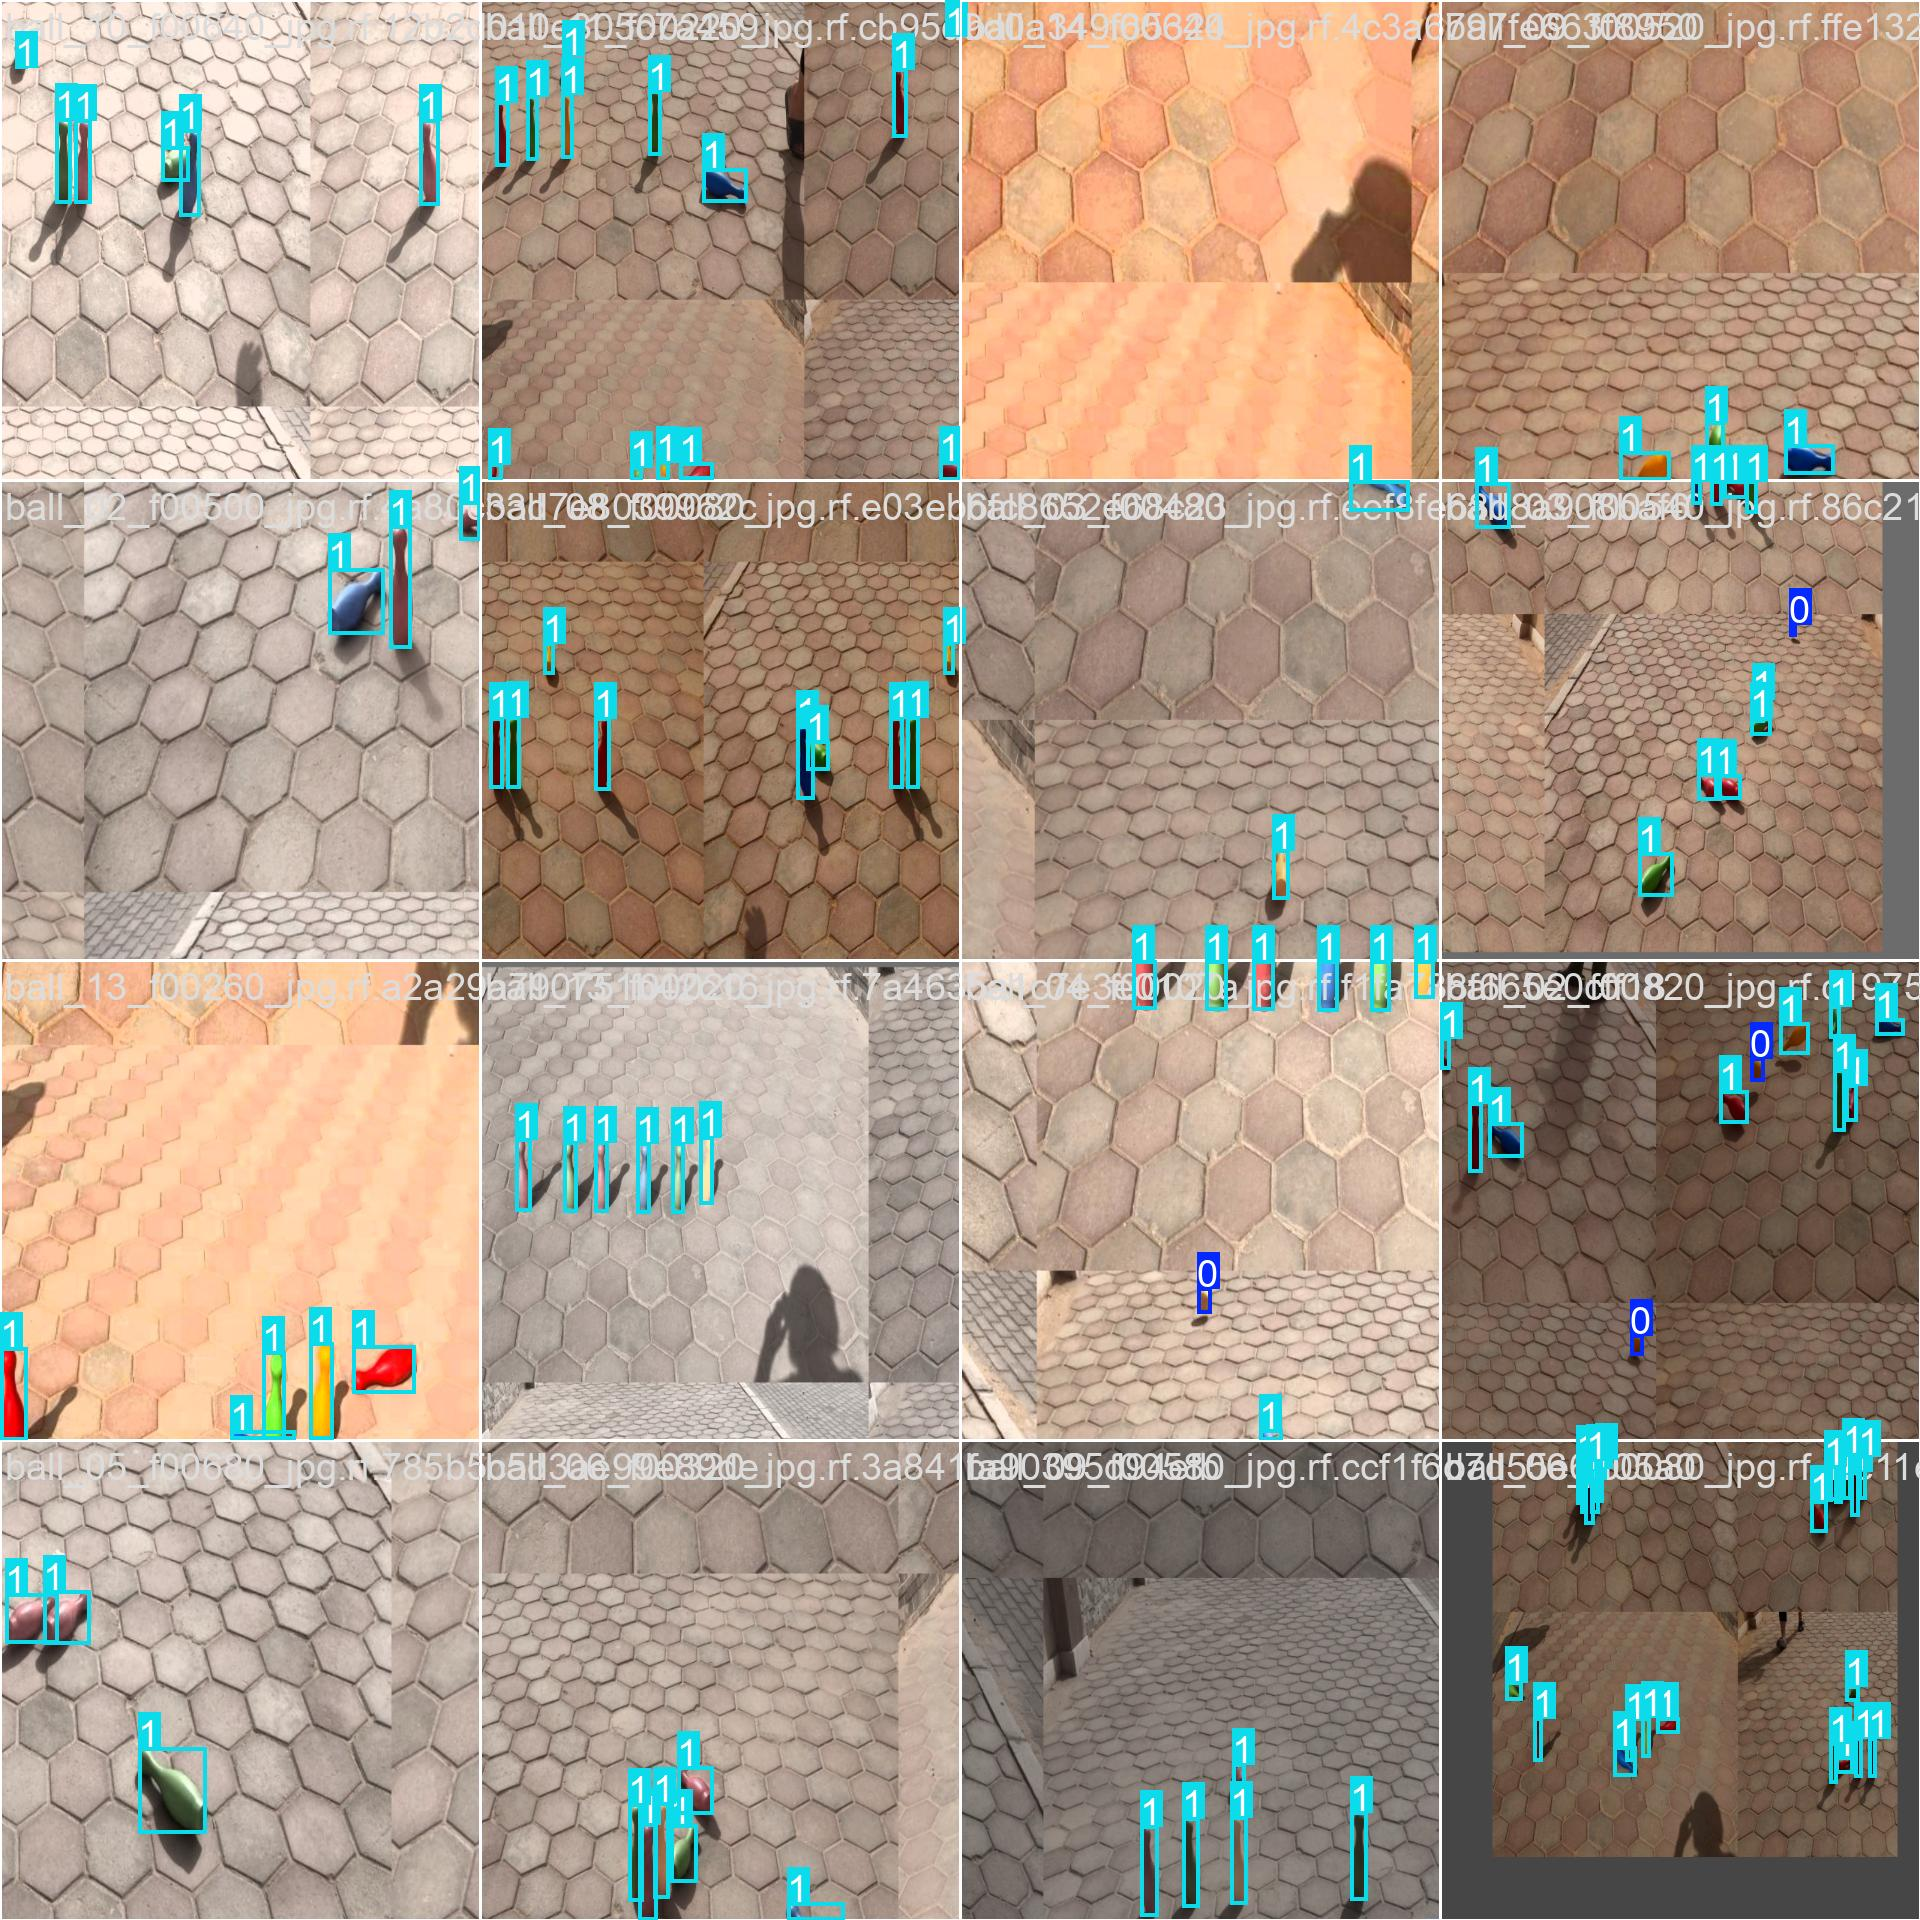
\includegraphics[width=0.32\textwidth]{figures/train_batch1.jpg}
    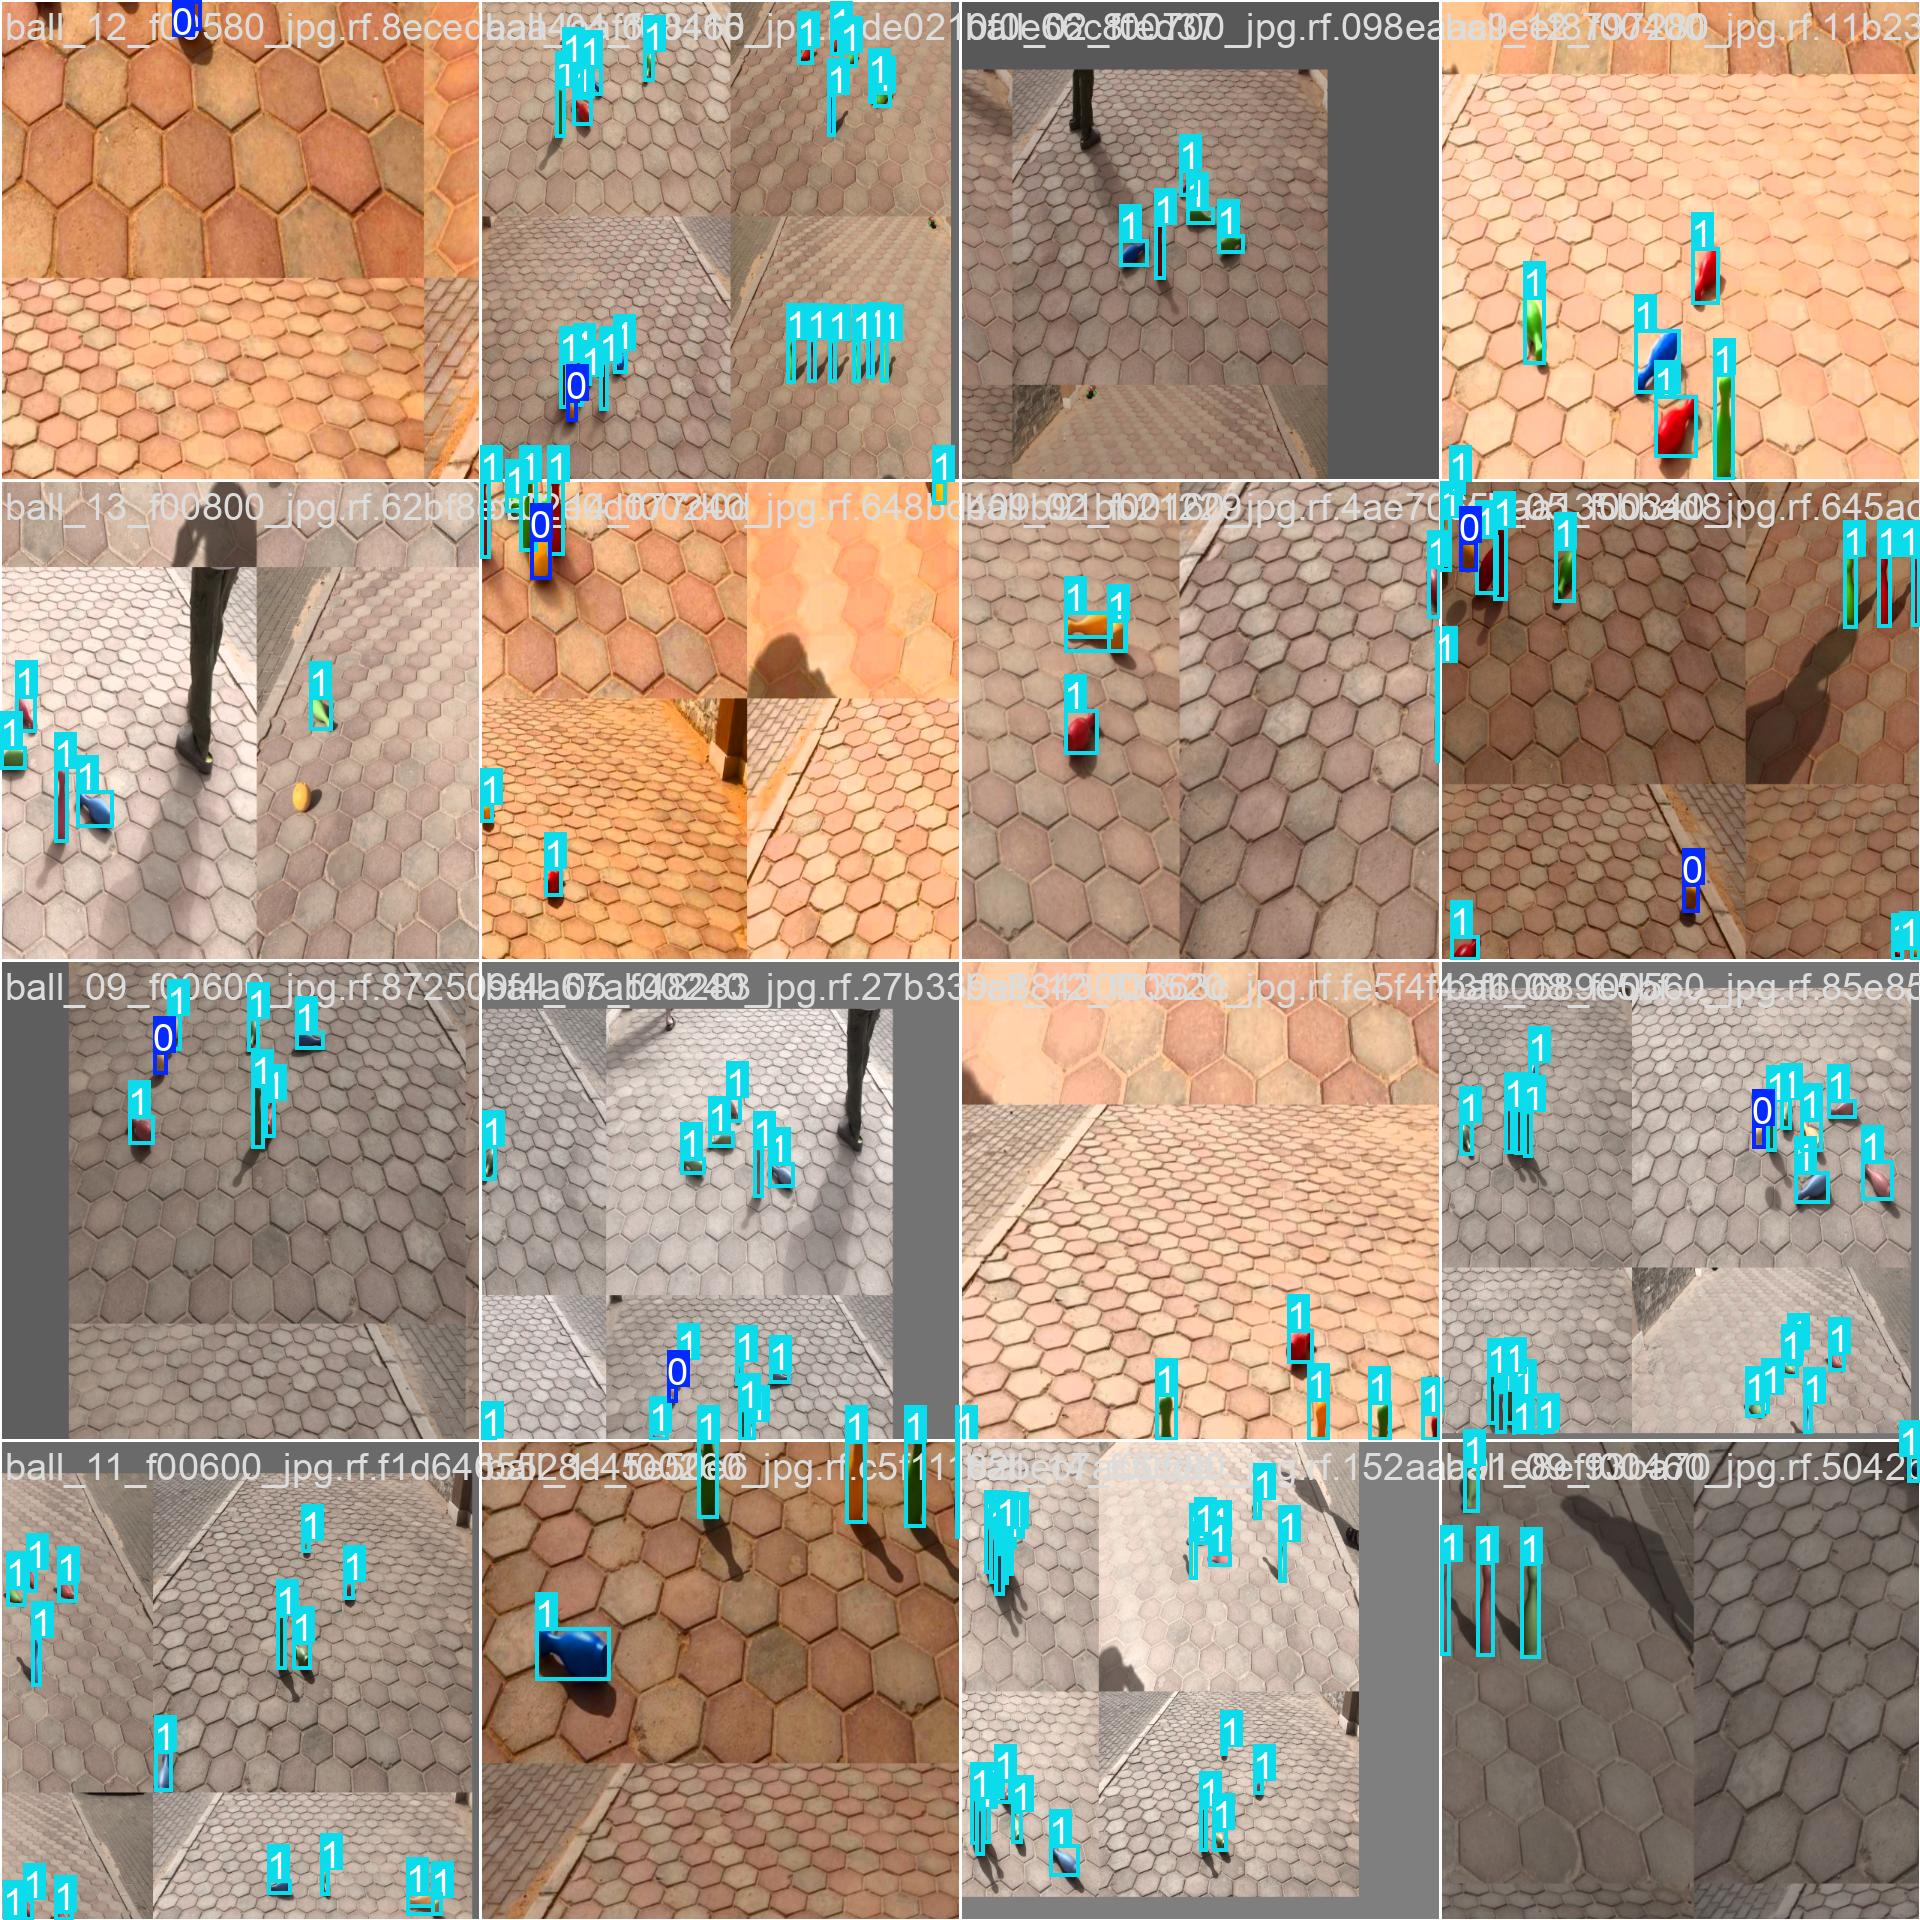
\includegraphics[width=0.32\textwidth]{figures/train_batch2.jpg}
    \caption{Initial Training Batches (0, 1, 2) demonstrating mosaic augmentation and the remediated bounding boxes overlaying the targets.}
\end{figure}

\begin{figure}[H]
    \centering
    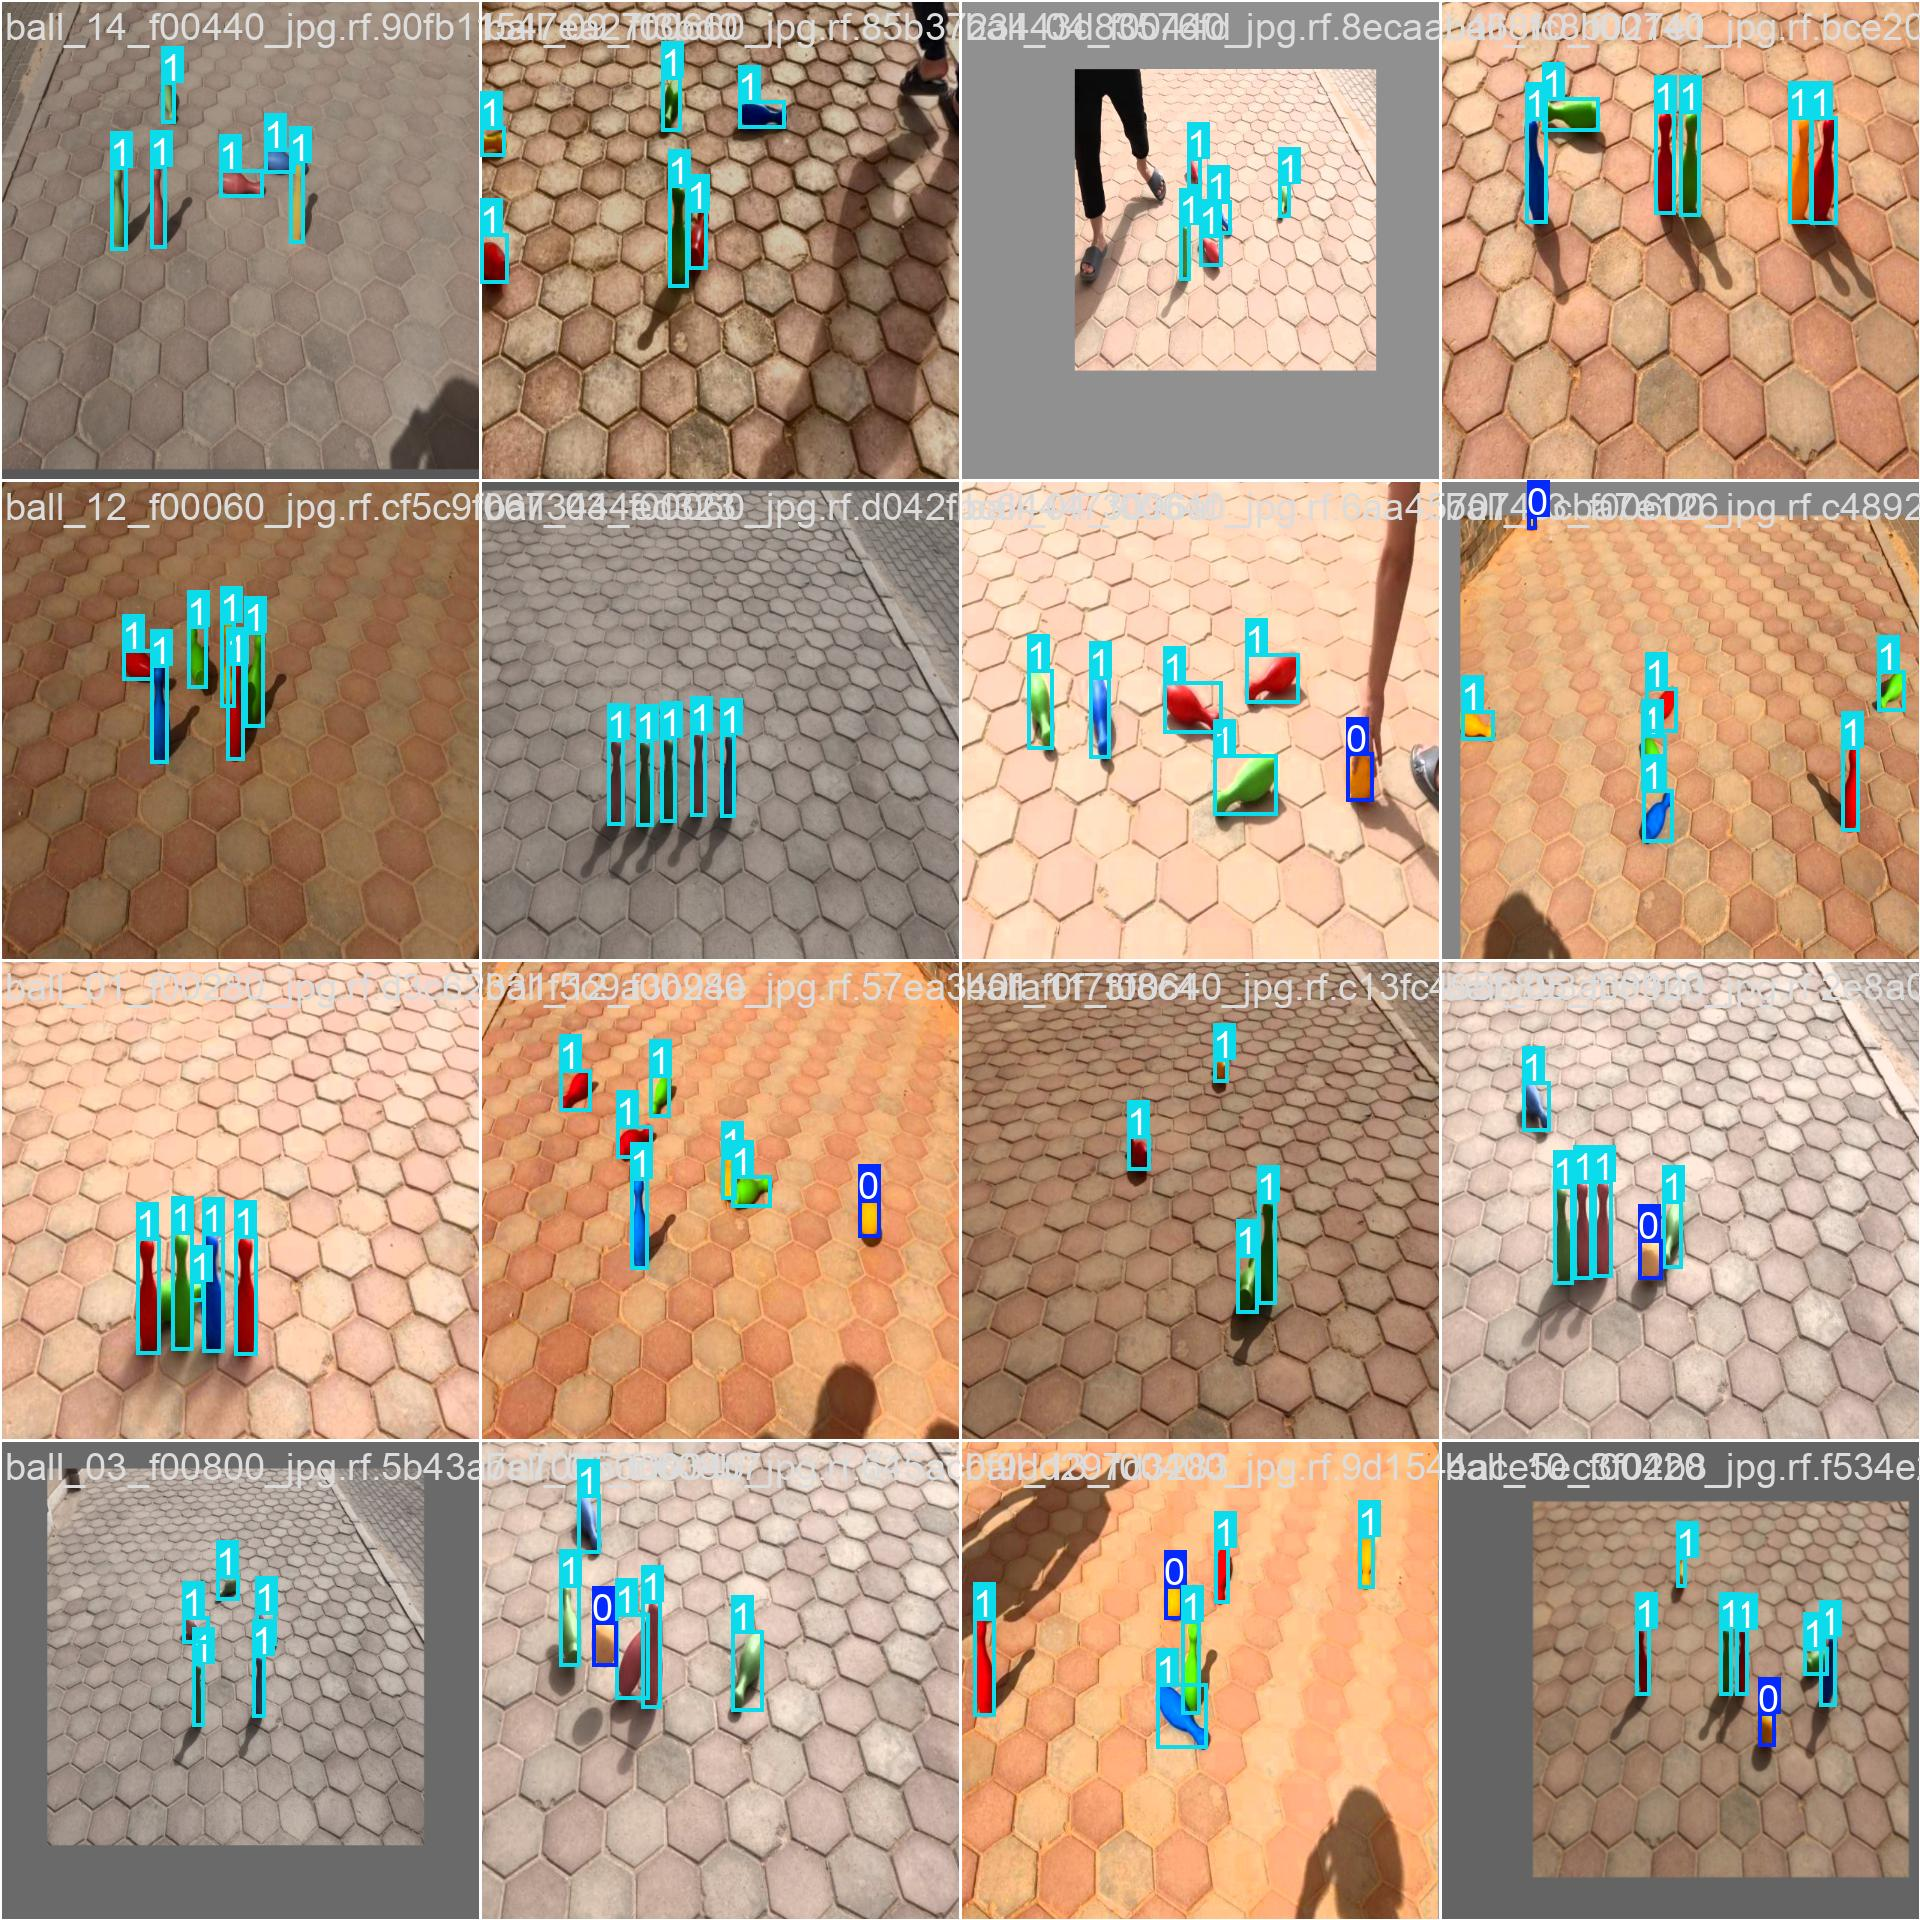
\includegraphics[width=0.32\textwidth]{figures/train_batch2340.jpg}
    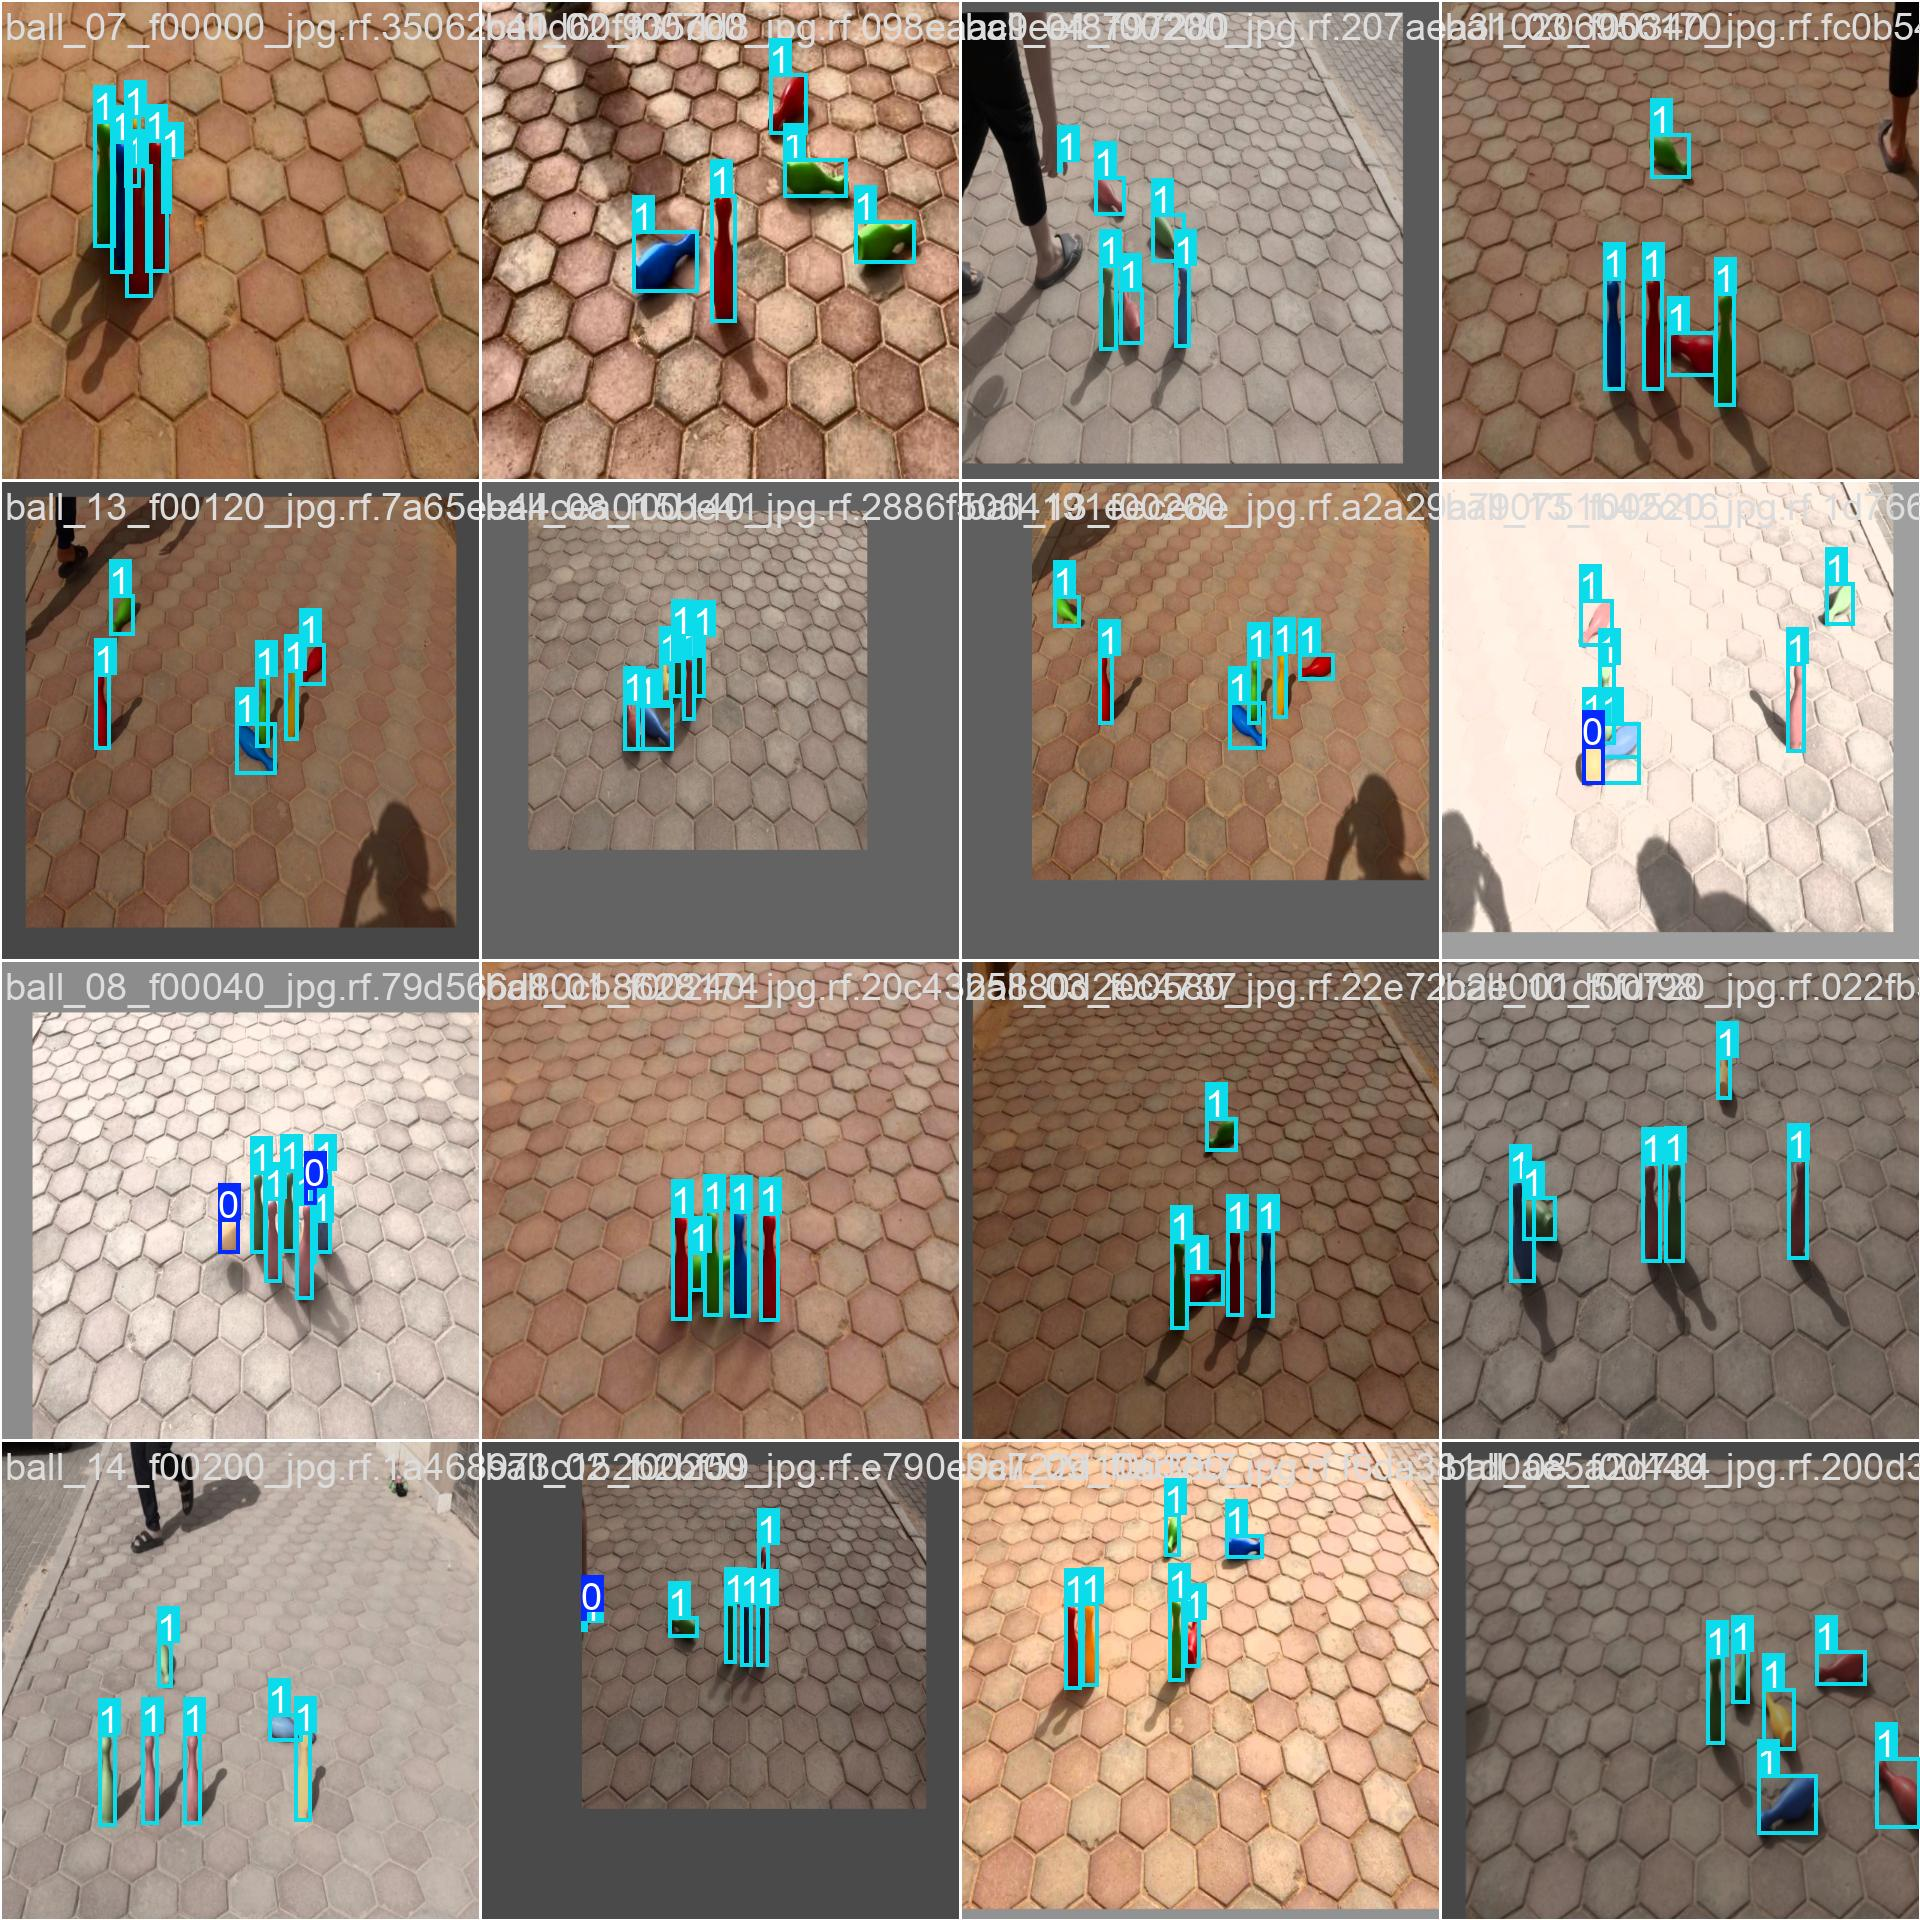
\includegraphics[width=0.32\textwidth]{figures/train_batch2341.jpg}
    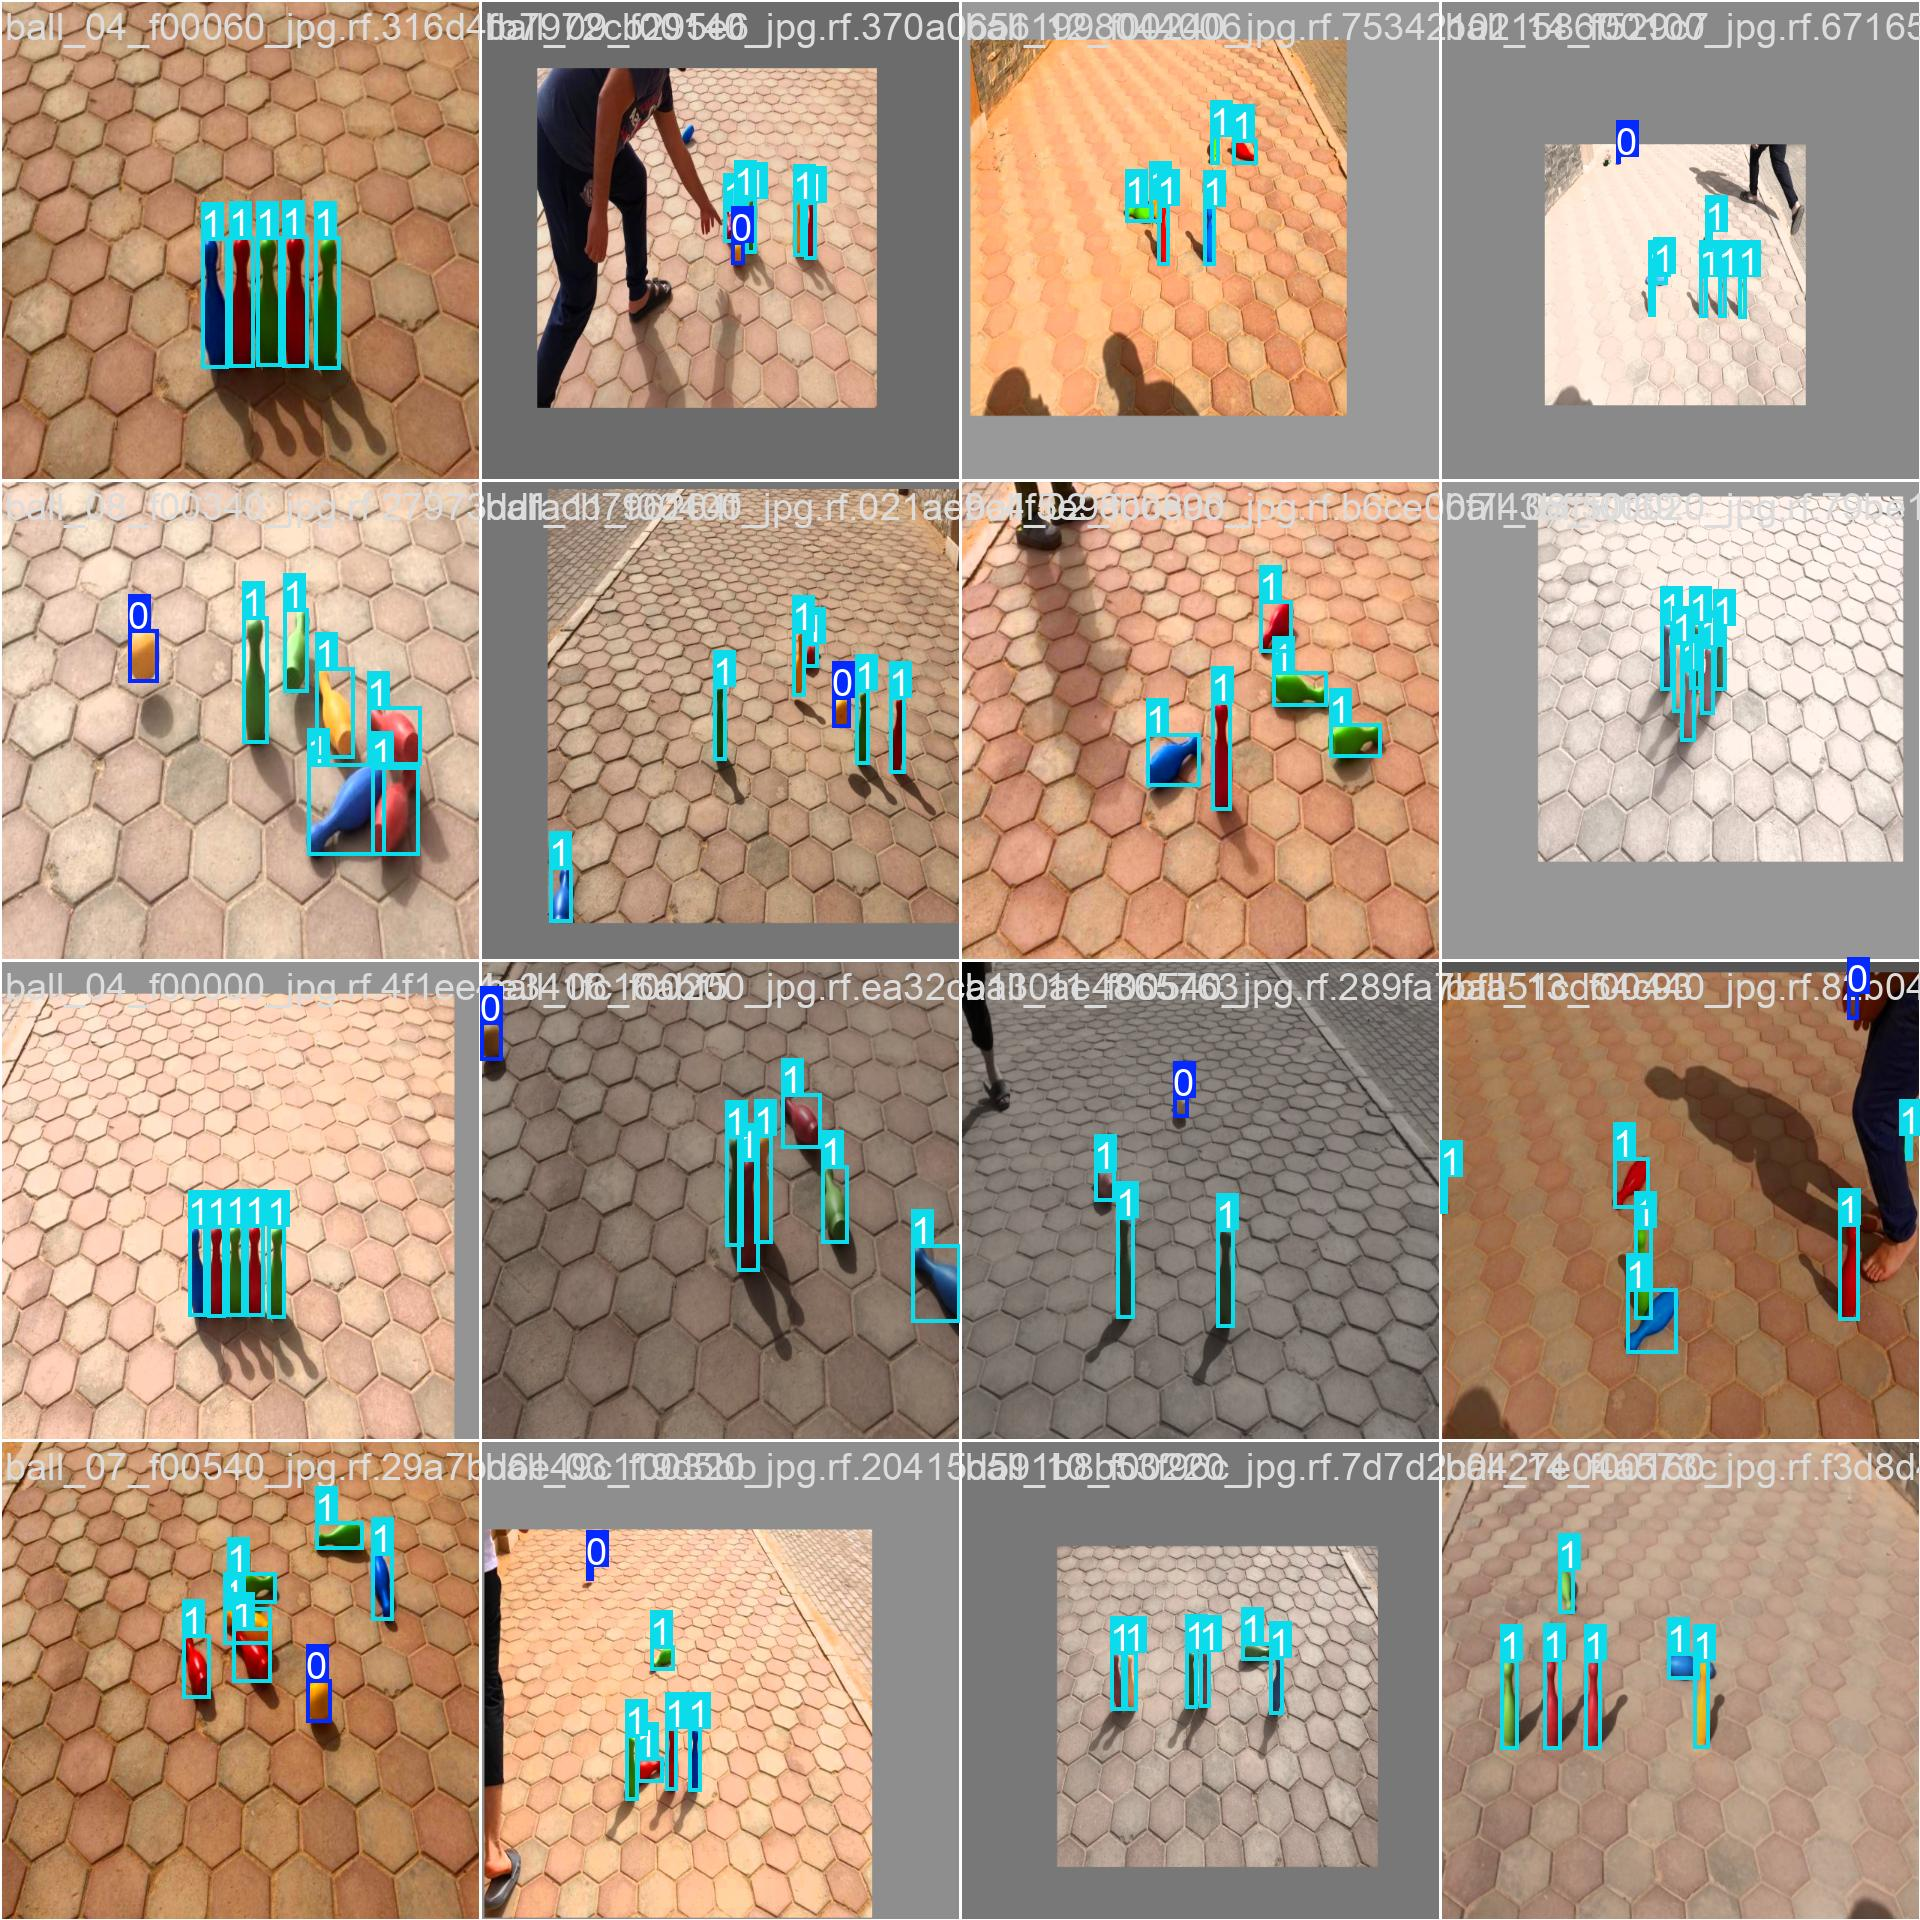
\includegraphics[width=0.32\textwidth]{figures/train_batch2342.jpg}
    \caption{Final Training Batches (2340, 2341, 2342) from the closing epochs, where mosaic augmentation is typically disabled to fine-tune localization.}
\end{figure}

\subsection{Validation Ground Truth vs. Predictions}
To visually confirm the model's accuracy, the validation set ground truths were plotted against the network's predictions.
\begin{figure}[H]
    \centering
    \begin{minipage}{0.48\textwidth}
        \centering
        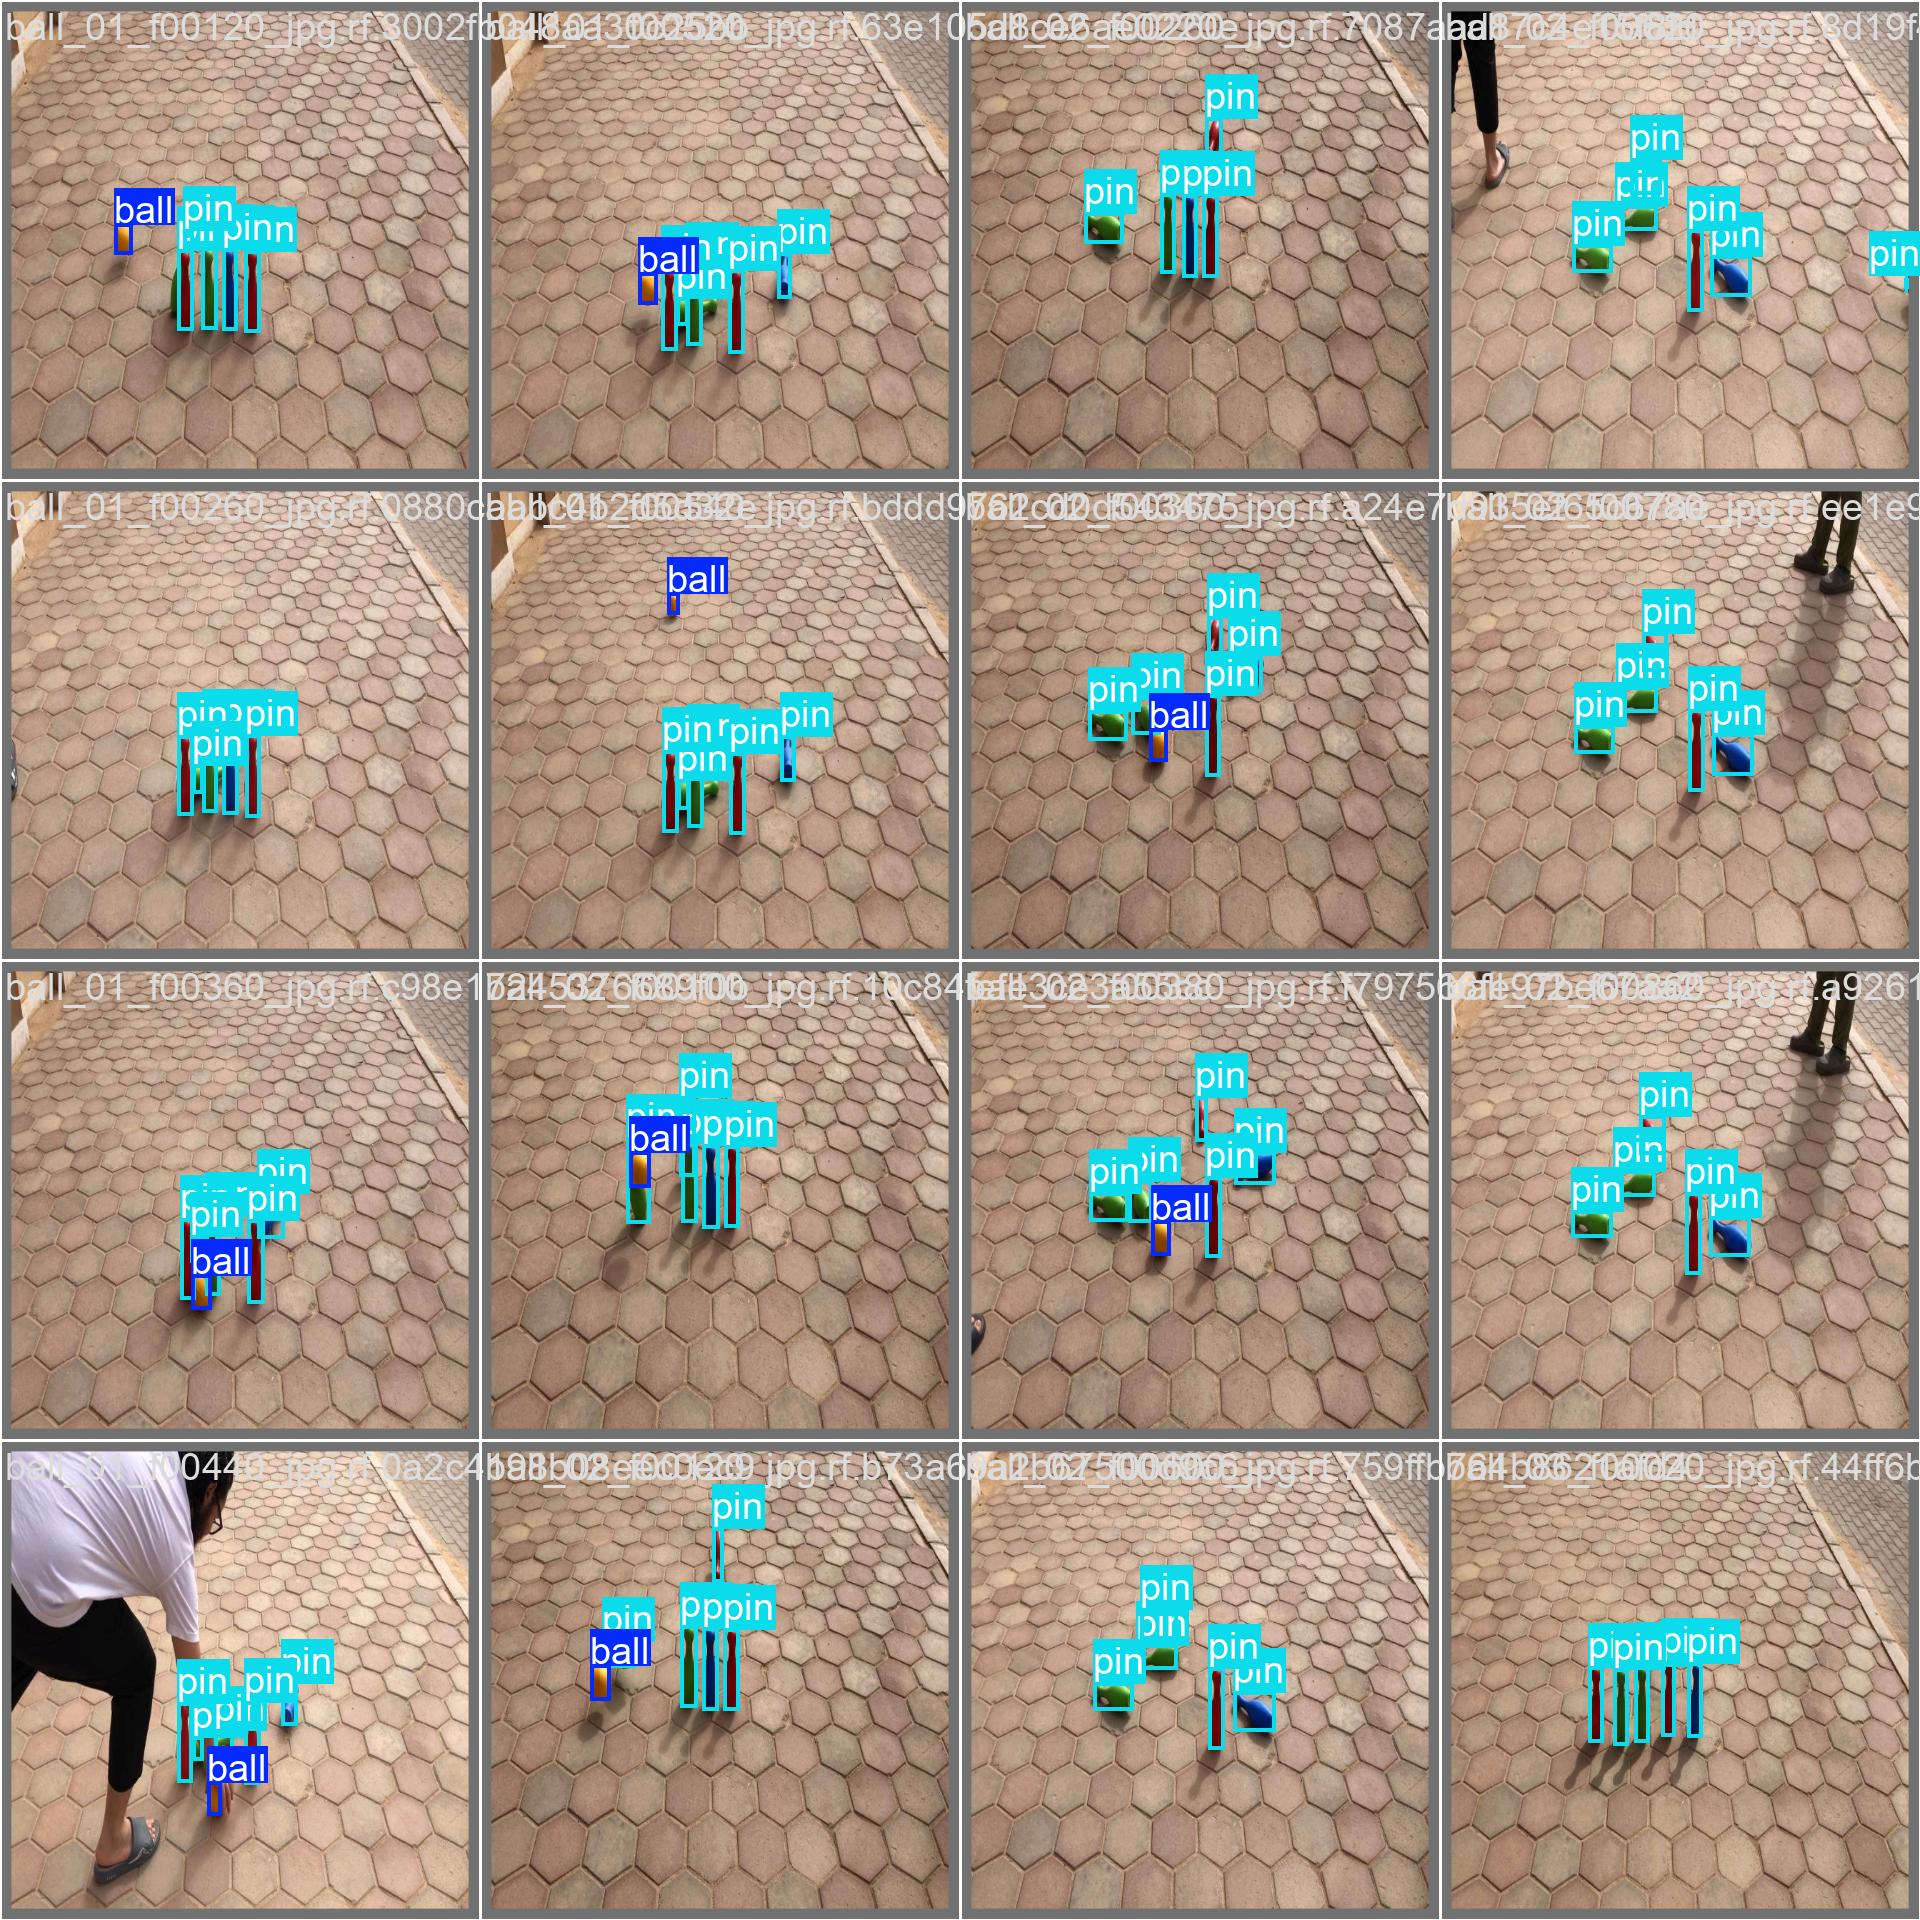
\includegraphics[width=\textwidth]{figures/val_batch0_labels.jpg}
        \caption{Validation Batch 0: Ground Truth Labels}
    \end{minipage}\hfill
    \begin{minipage}{0.48\textwidth}
        \centering
        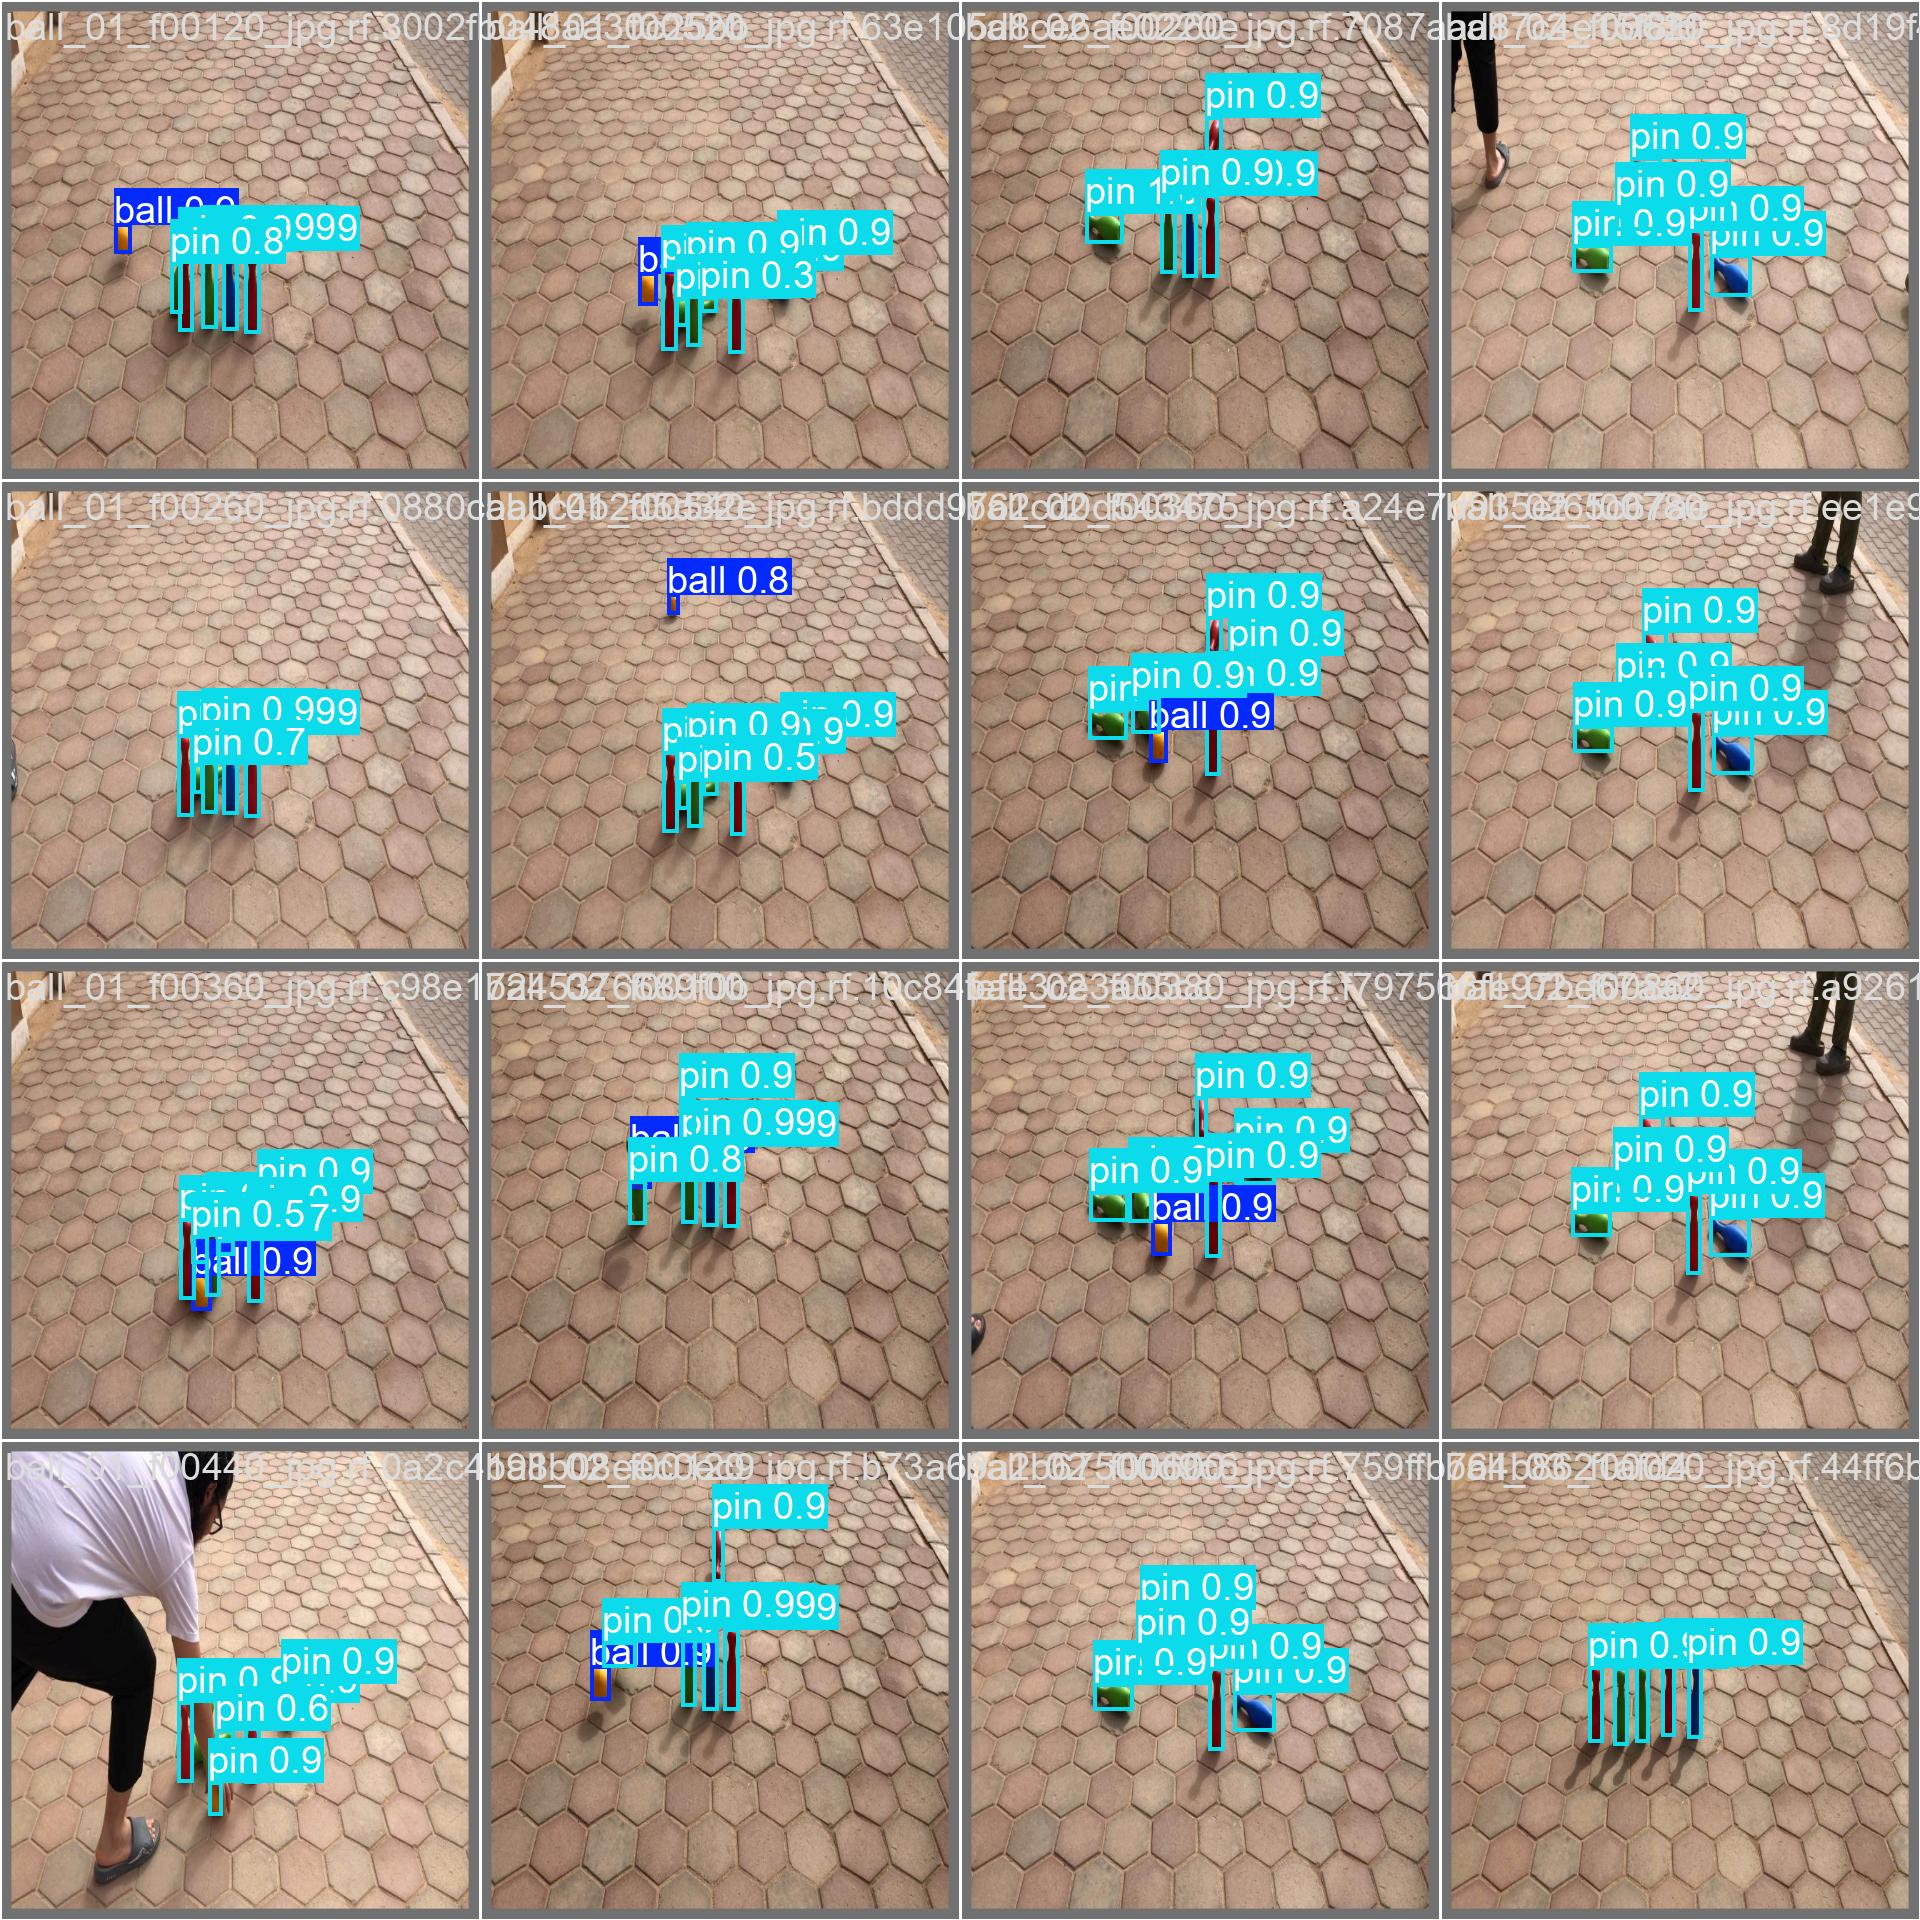
\includegraphics[width=\textwidth]{figures/val_batch0_pred.jpg}
        \caption{Validation Batch 0: Model Predictions}
    \end{minipage}
\end{figure}

\begin{figure}[H]
    \centering
    \begin{minipage}{0.48\textwidth}
        \centering
        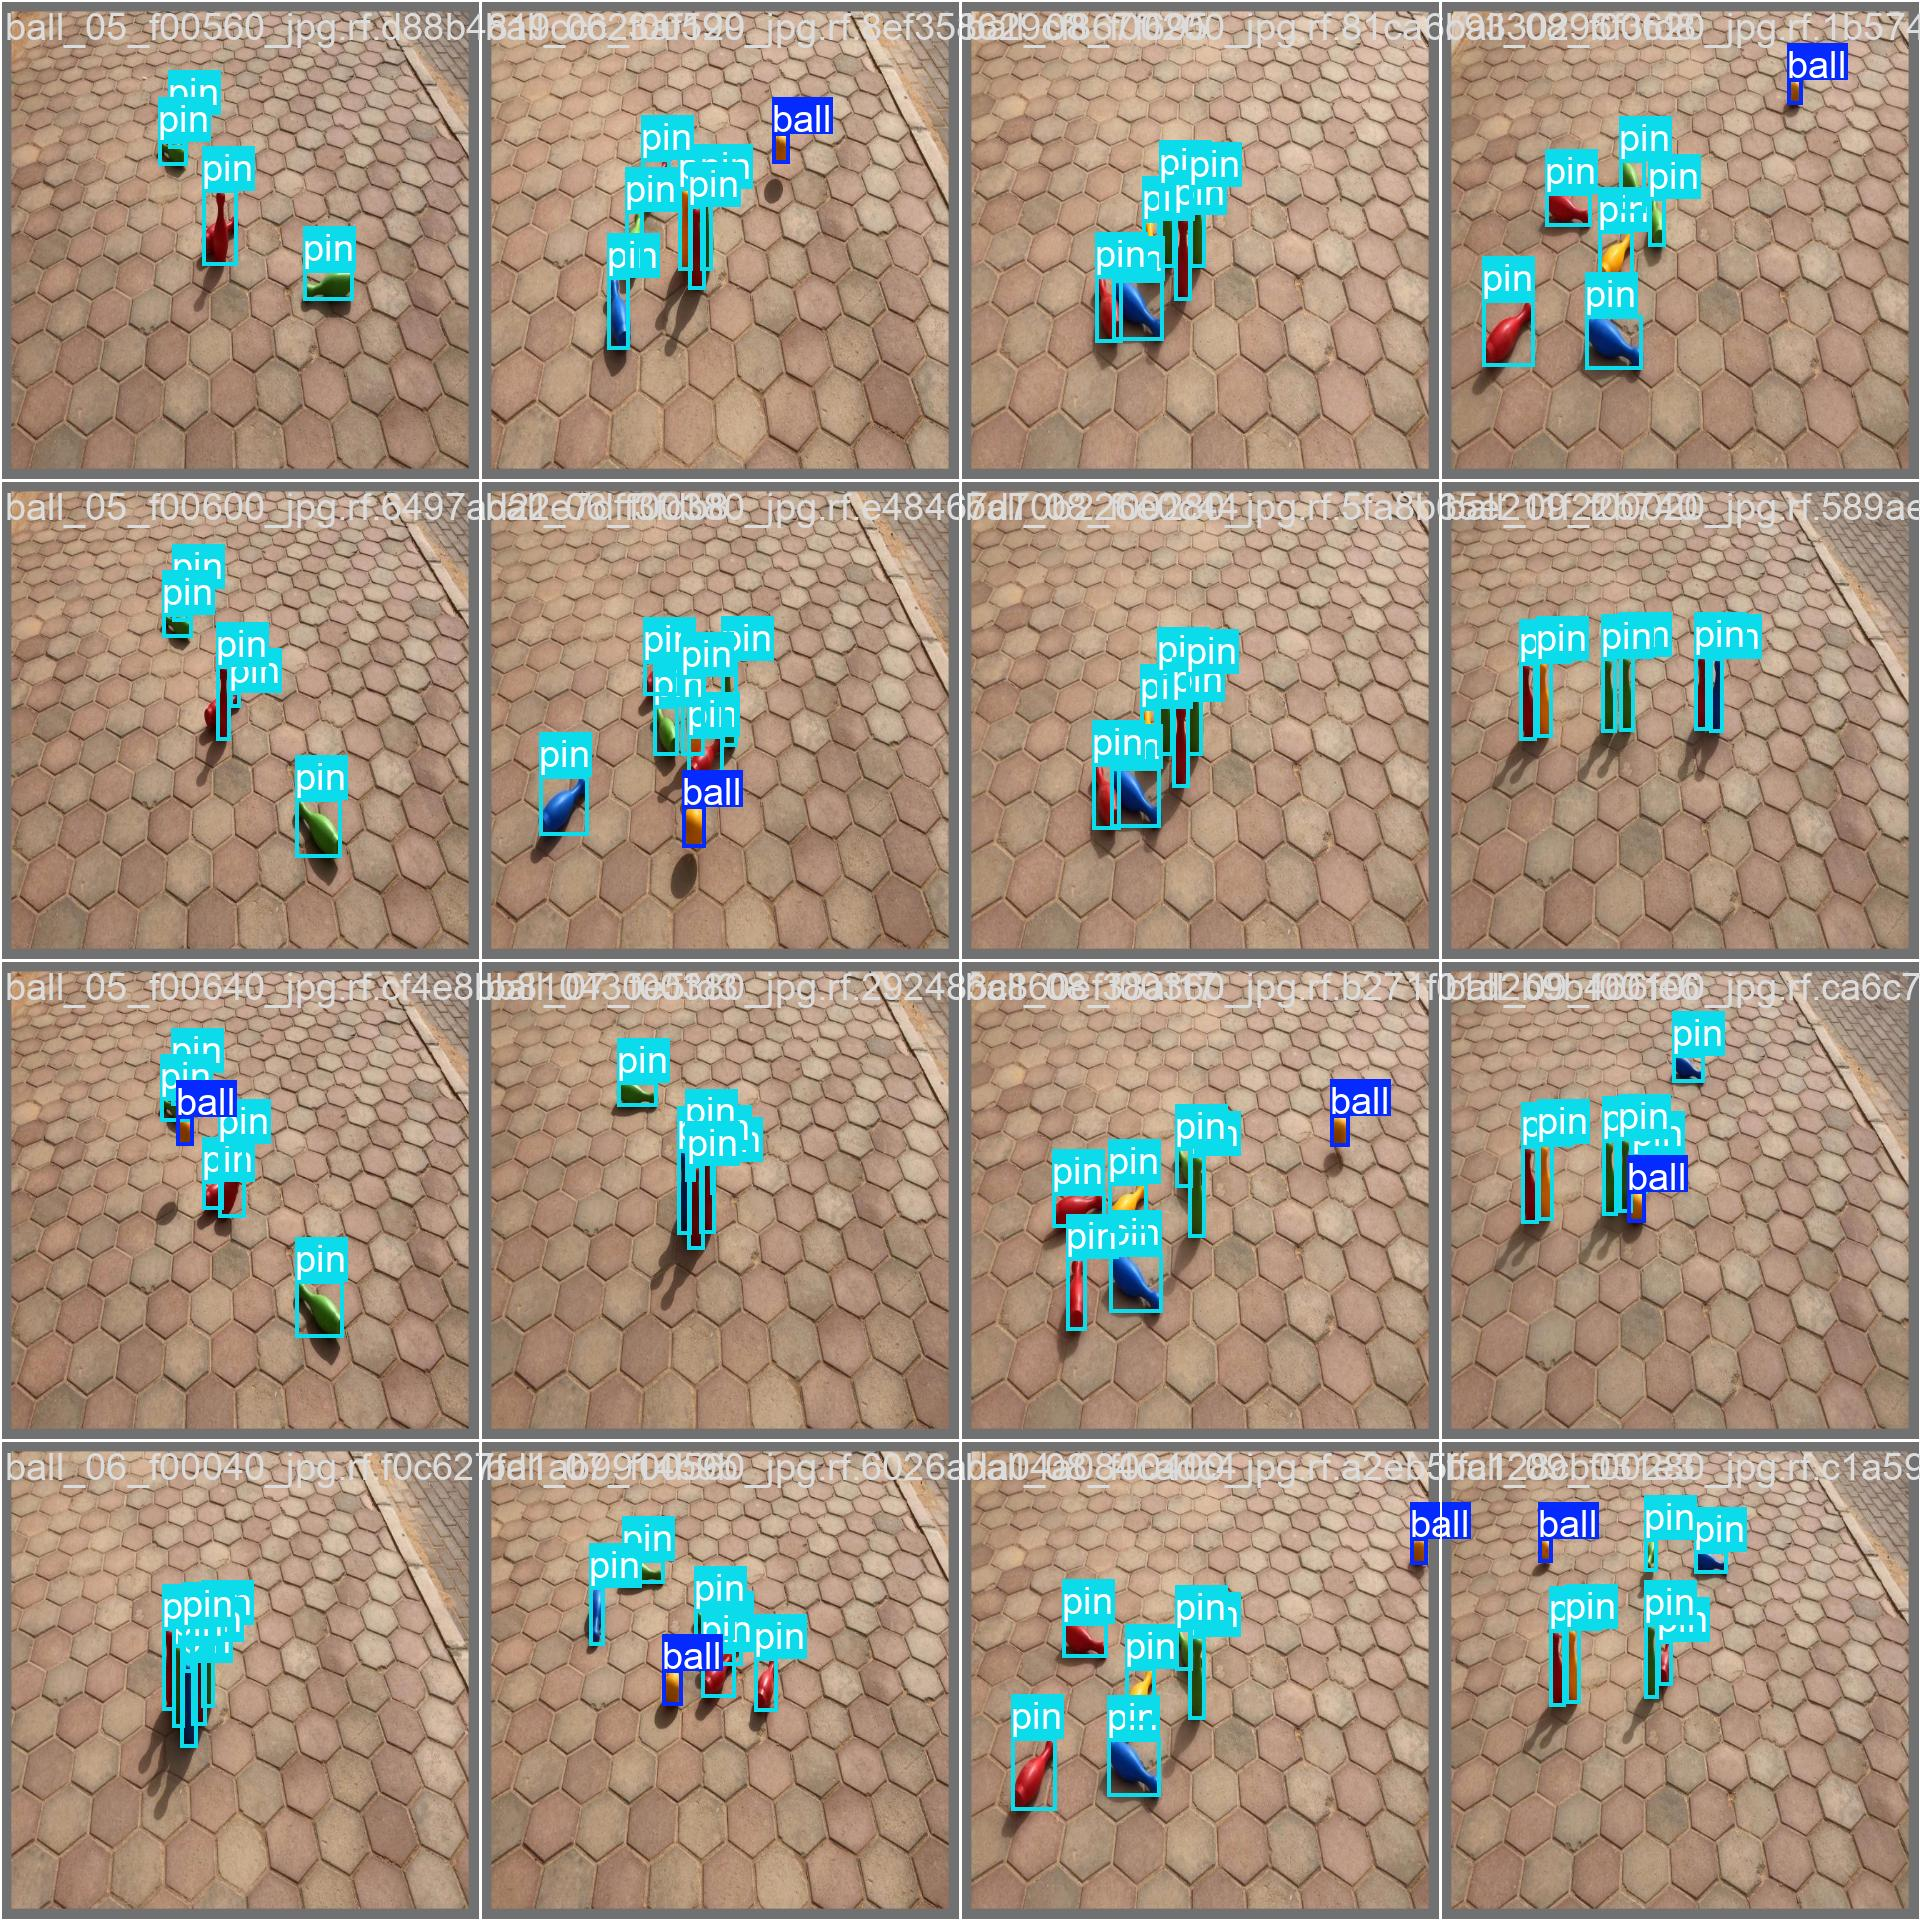
\includegraphics[width=\textwidth]{figures/val_batch1_labels.jpg}
        \caption{Validation Batch 1: Ground Truth Labels}
    \end{minipage}\hfill
    \begin{minipage}{0.48\textwidth}
        \centering
        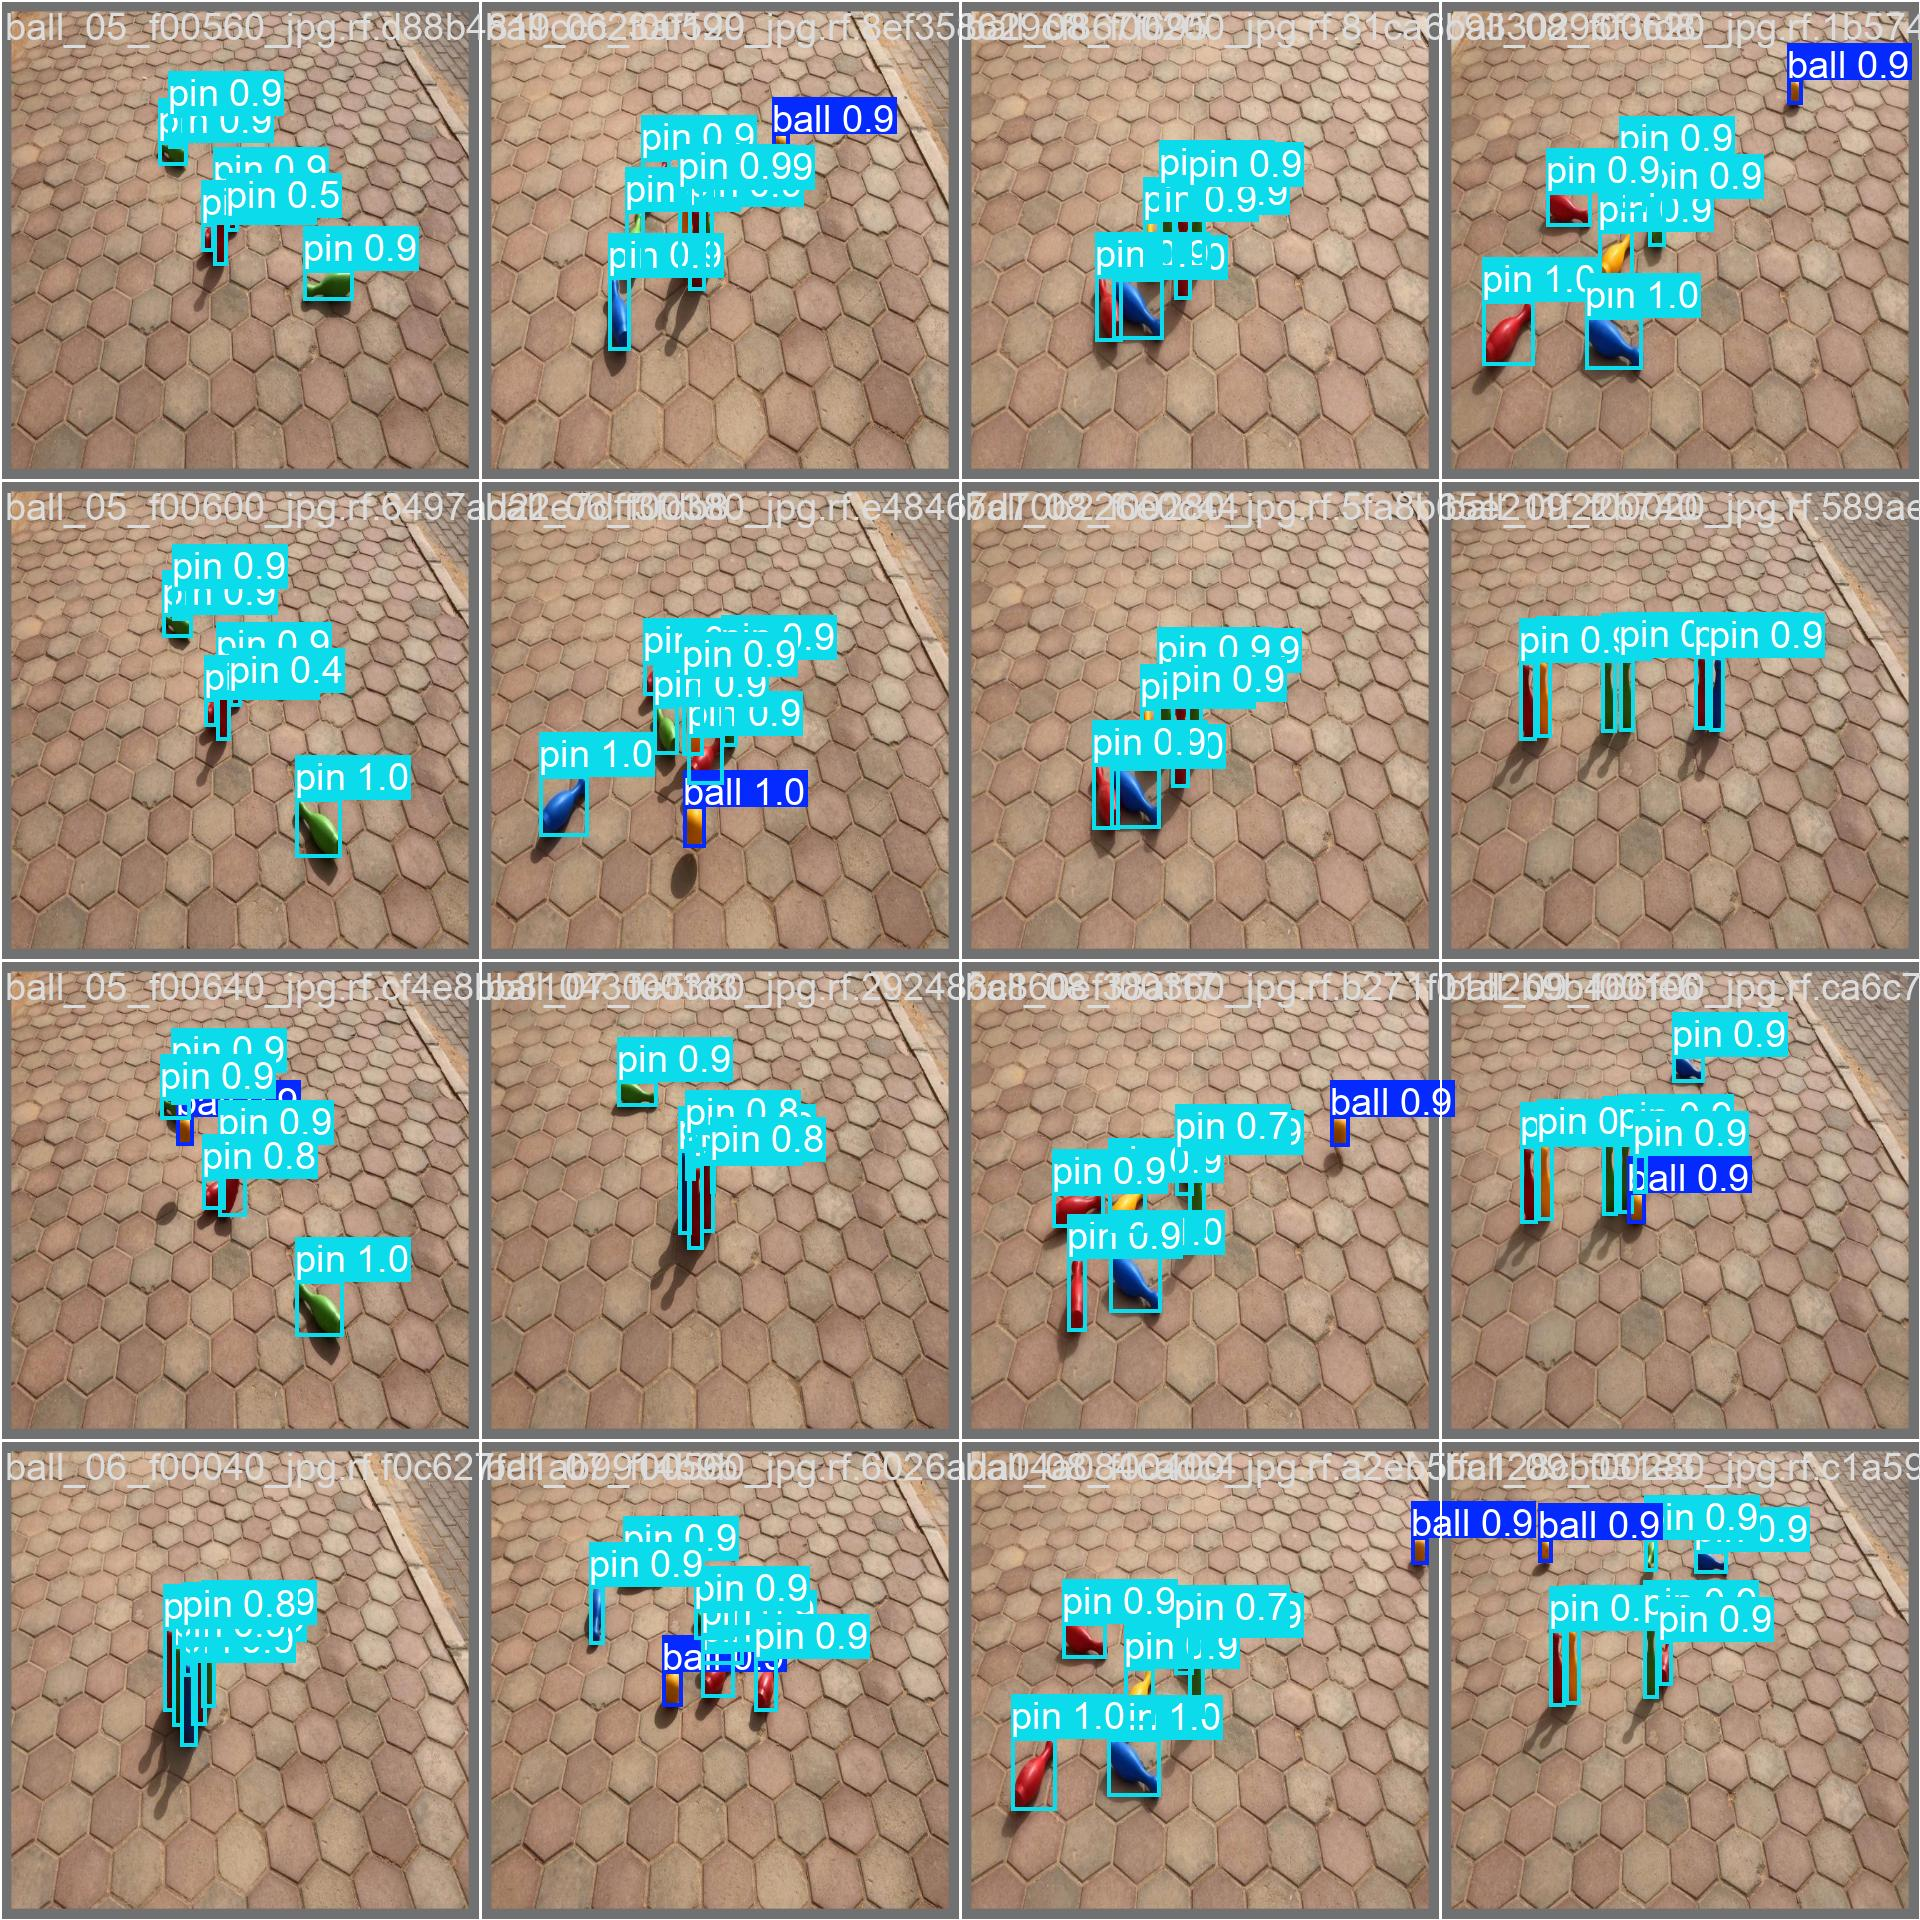
\includegraphics[width=\textwidth]{figures/val_batch1_pred.jpg}
        \caption{Validation Batch 1: Model Predictions}
    \end{minipage}
\end{figure}

\begin{figure}[H]
    \centering
    \begin{minipage}{0.48\textwidth}
        \centering
        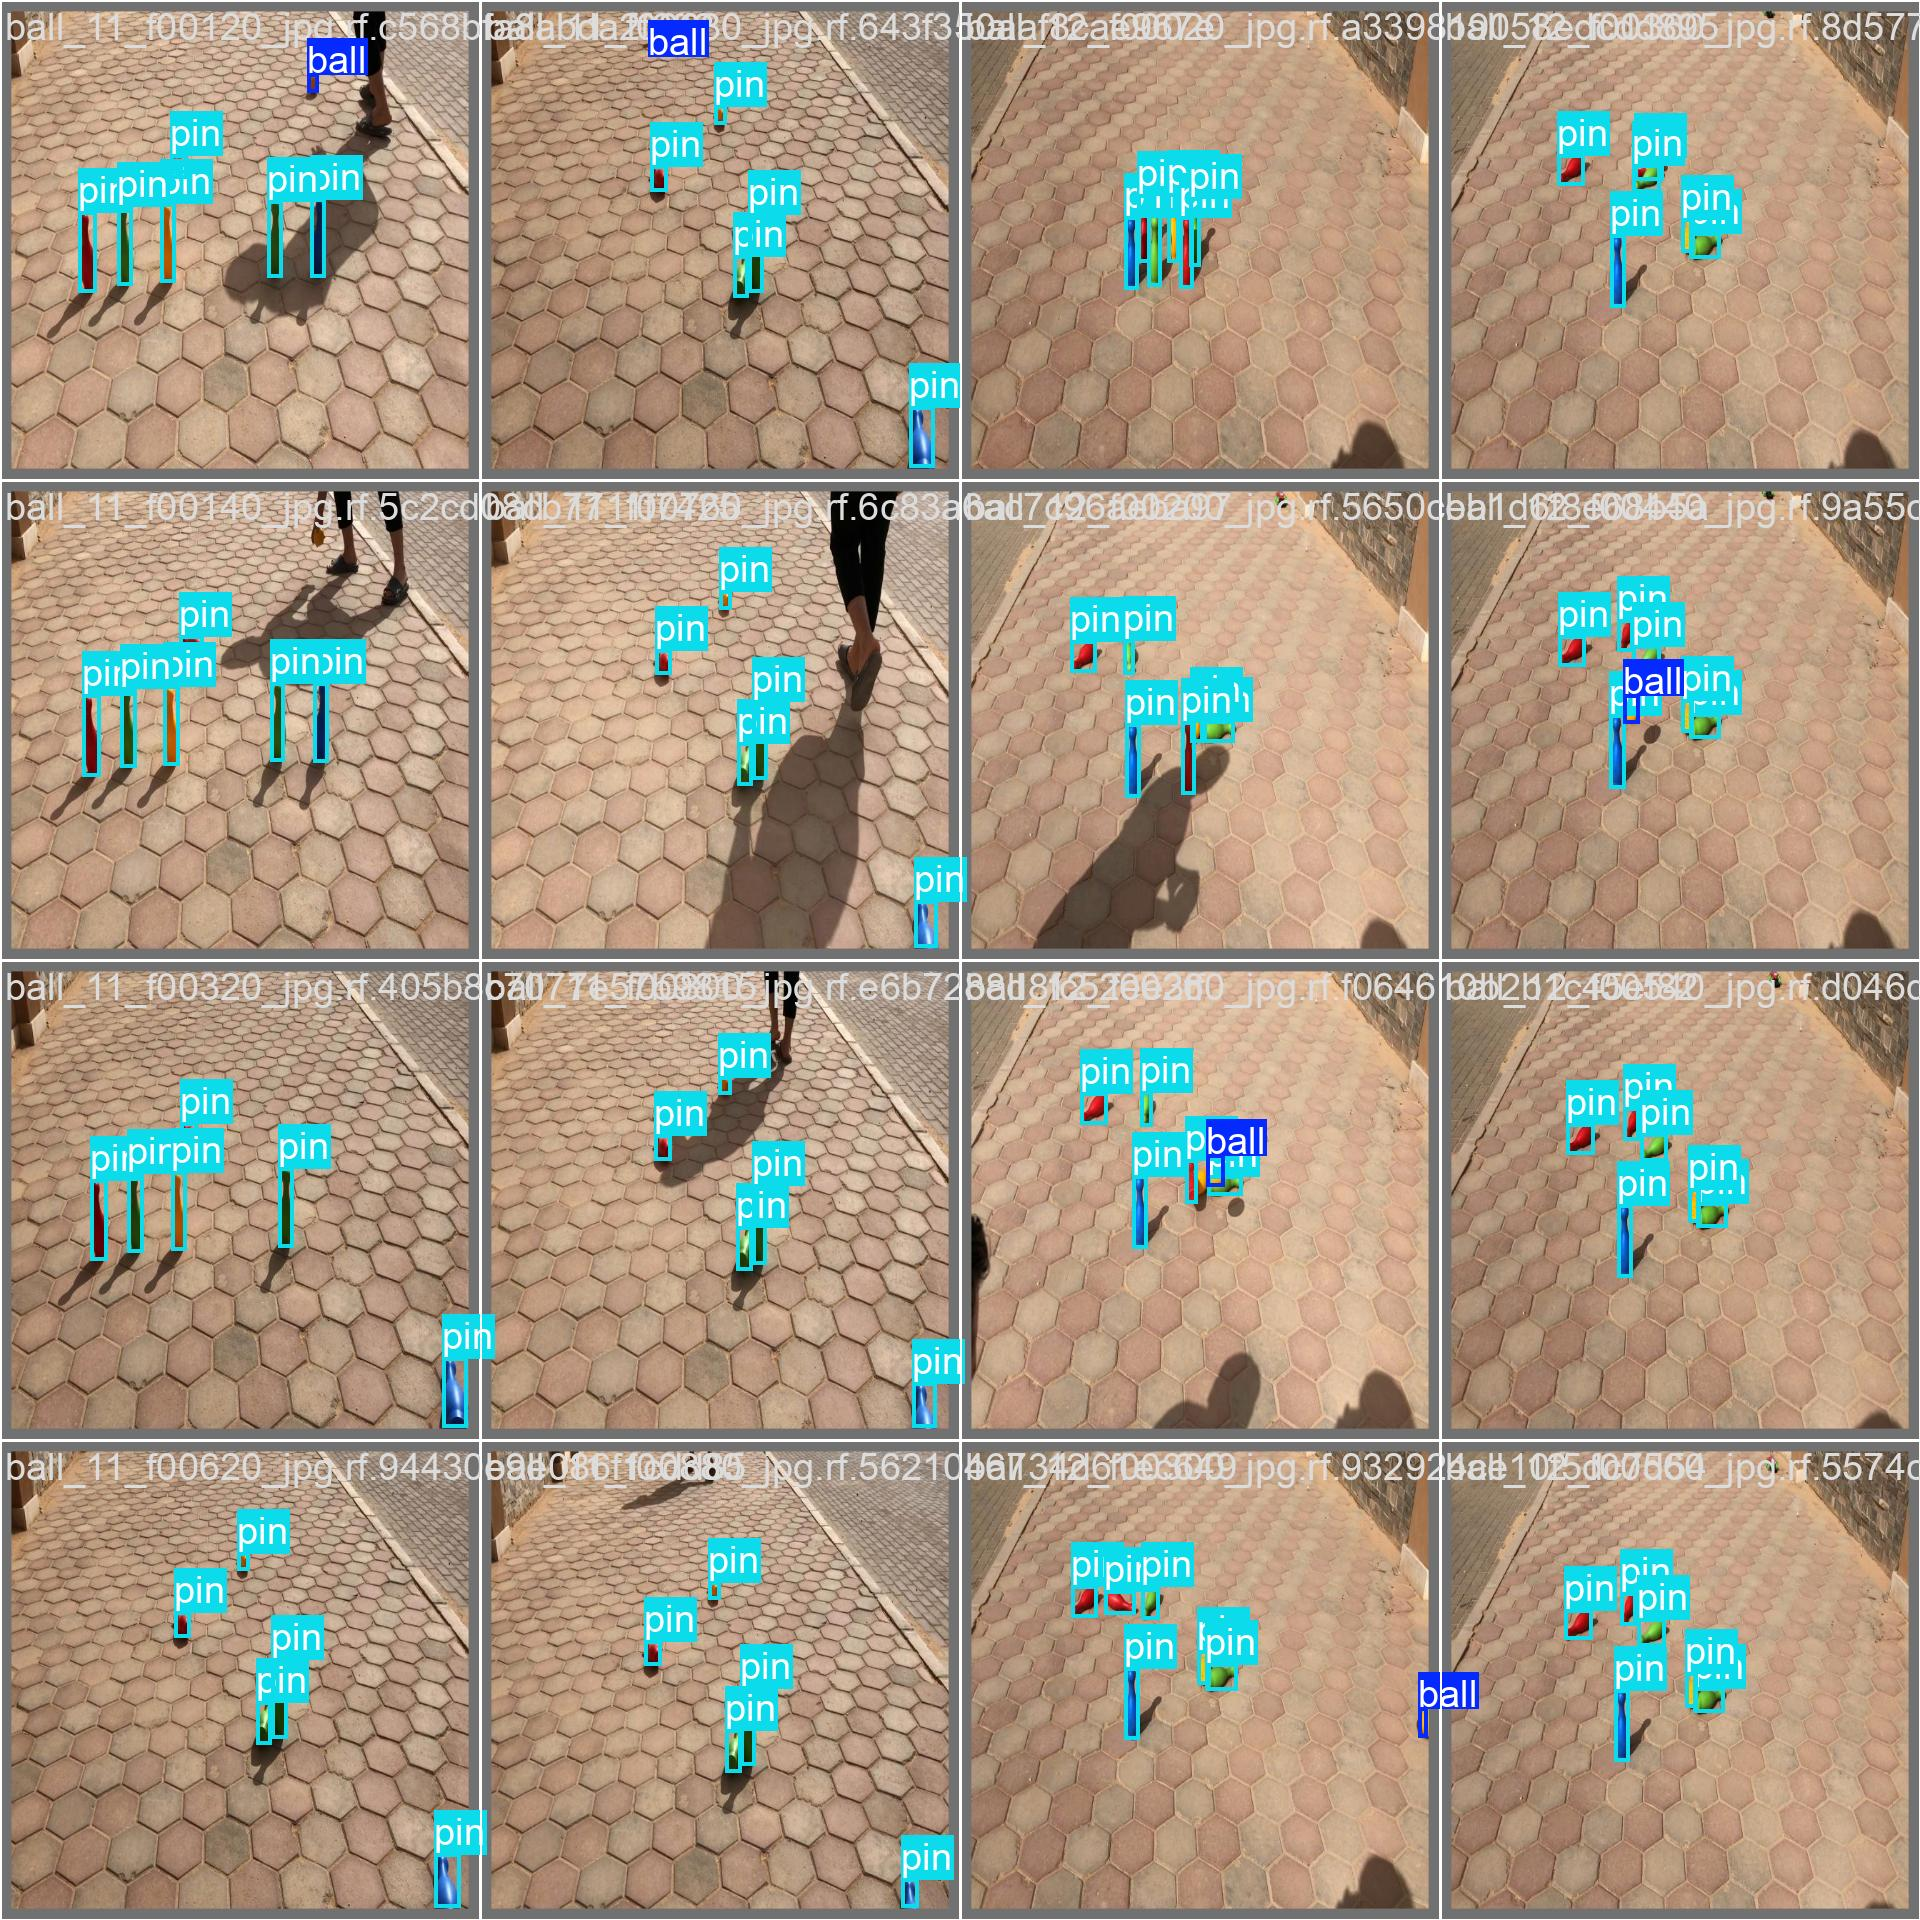
\includegraphics[width=\textwidth]{figures/val_batch2_labels.jpg}
        \caption{Validation Batch 2: Ground Truth Labels}
    \end{minipage}\hfill
    \begin{minipage}{0.48\textwidth}
        \centering
        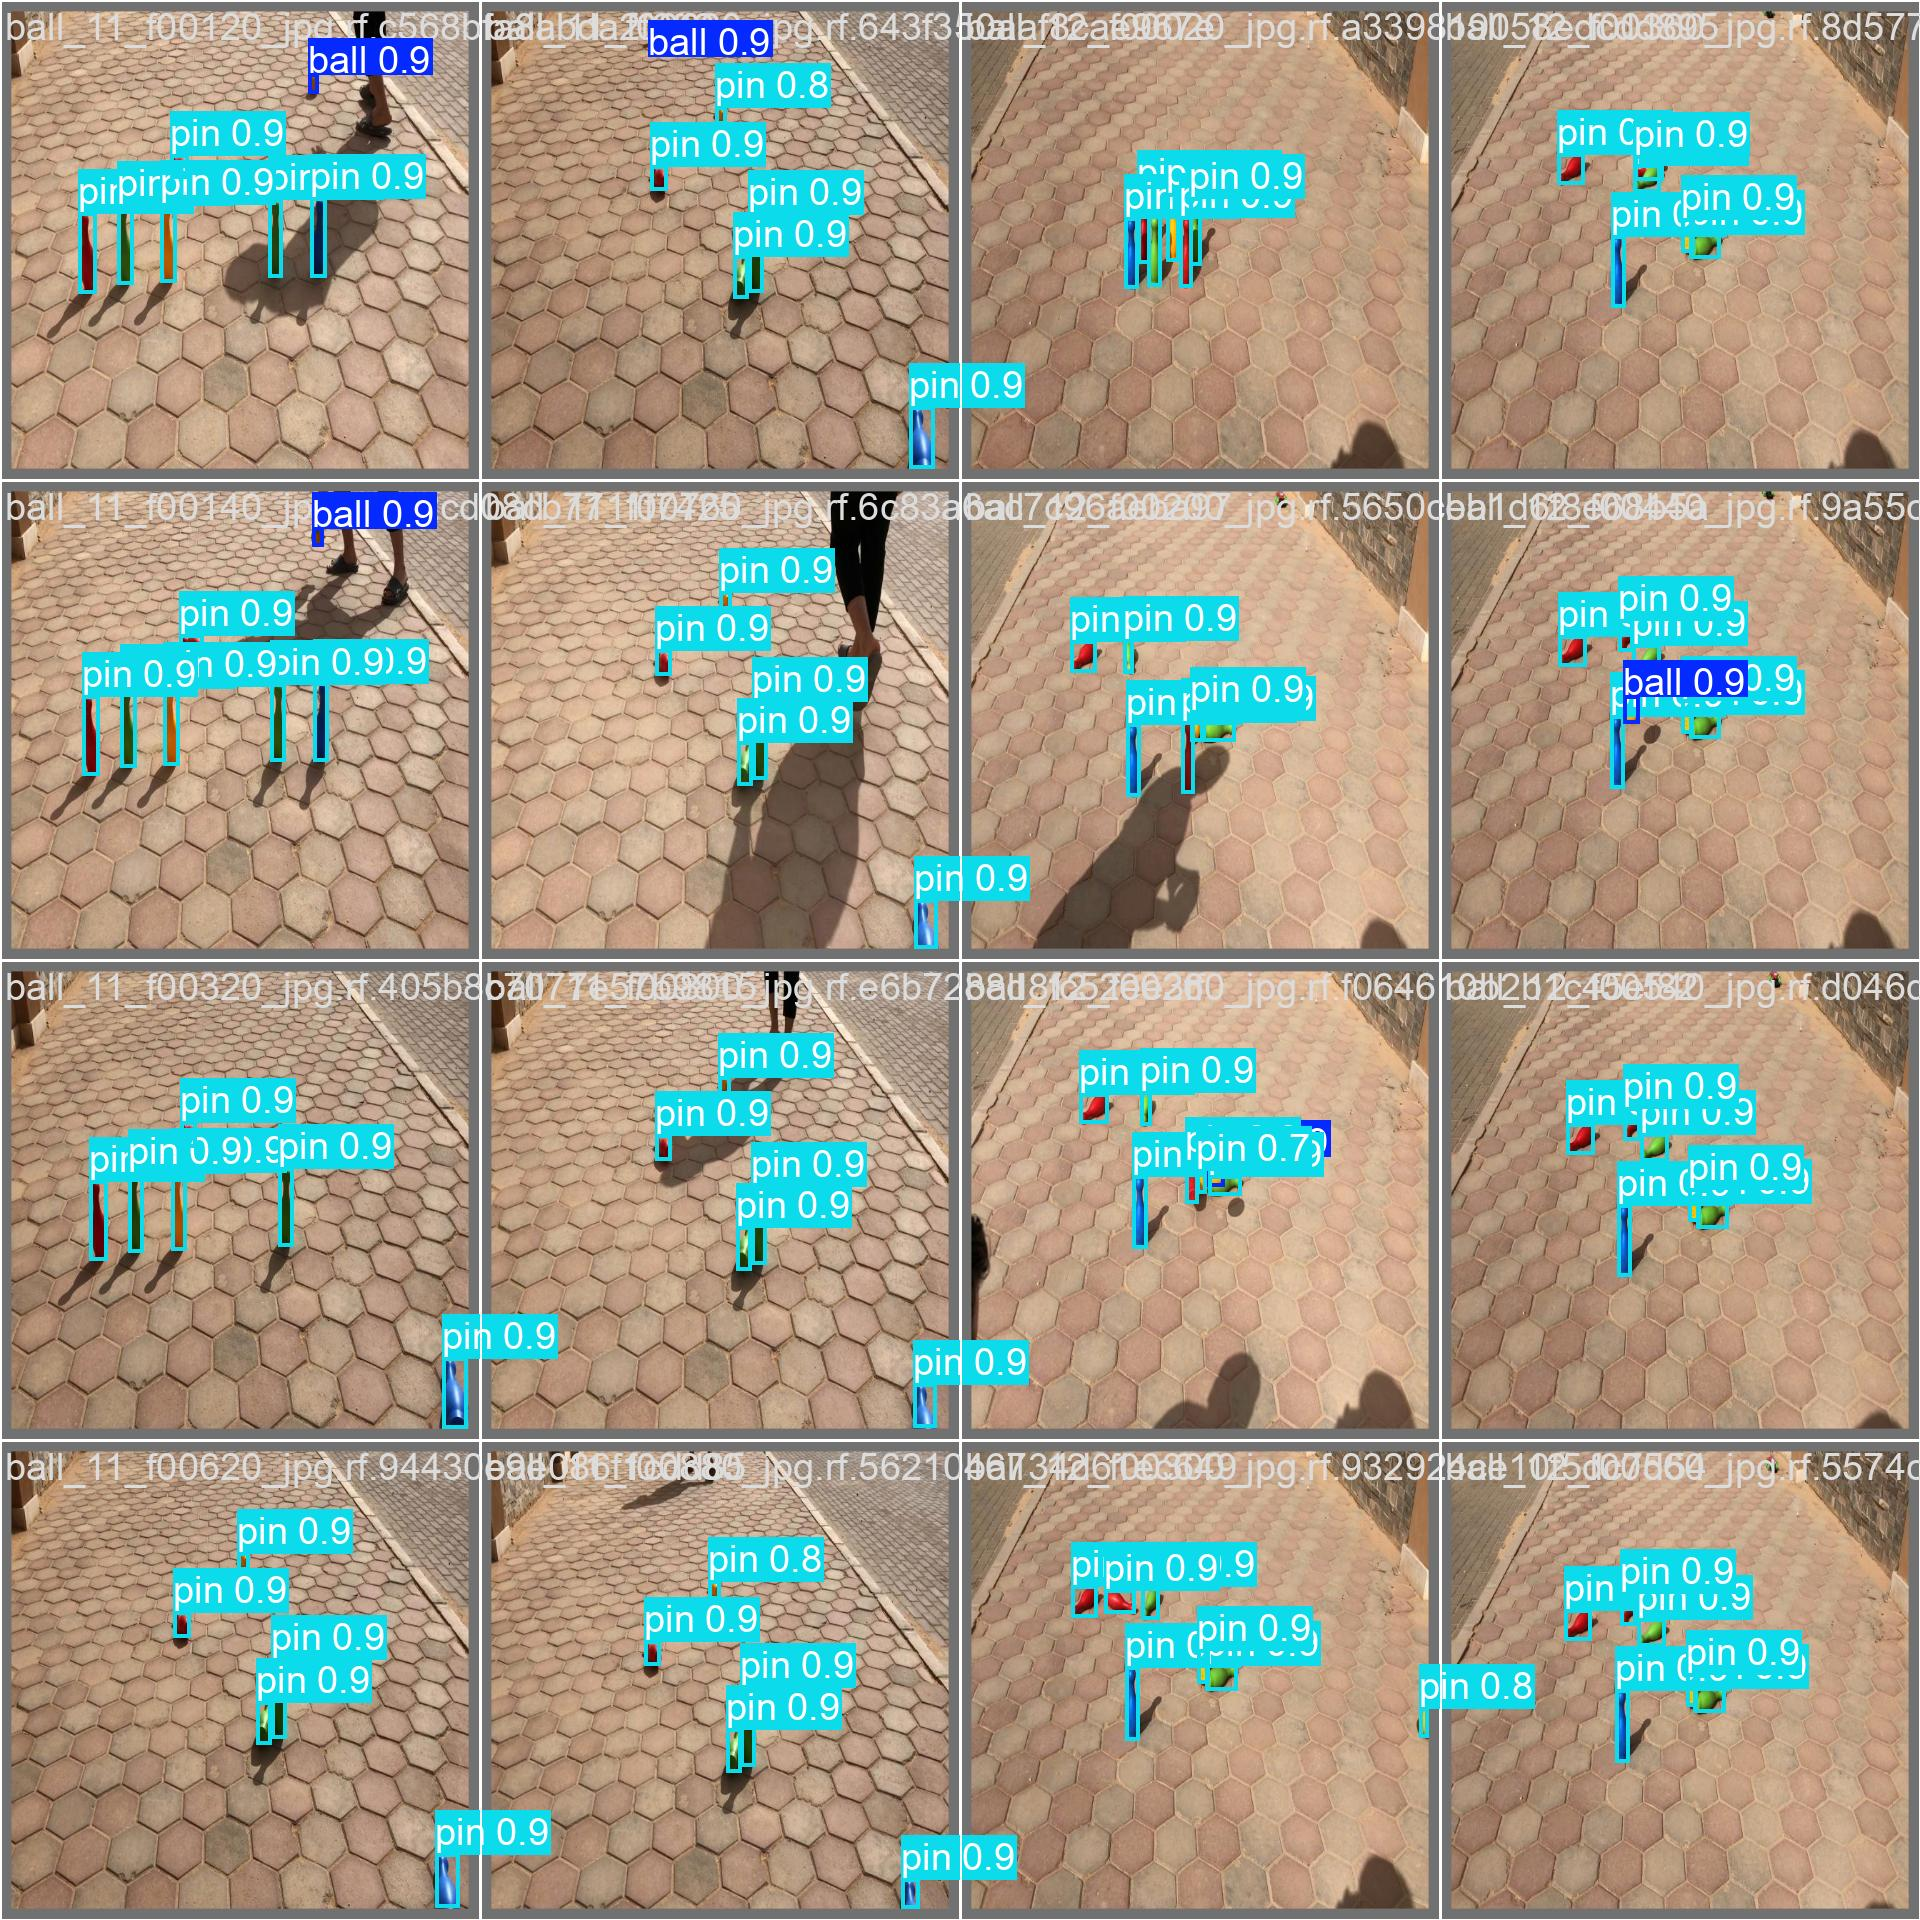
\includegraphics[width=\textwidth]{figures/val_batch2_pred.jpg}
        \caption{Validation Batch 2: Model Predictions}
    \end{minipage}
\end{figure}

\subsection{Quantitative Metrics and Performance Curves}
Evaluation yielded exceptional quantitative metrics recorded in \texttt{main\_metrics.json} and \texttt{results.csv}:
\begin{table}[H]
\centering
\begin{tabular}{@{}ll@{}}
\toprule
\textbf{Metric} & \textbf{Value} \\ \midrule
mAP@0.5 & 0.9819 (98.19\%) \\
mAP@0.5:0.95 & 0.9383 (93.83\%) \\
Precision & 0.9297 \\
Recall & 0.9664 \\
Max F1-Score & 0.9477 at Confidence 0.1 \\ \bottomrule
\end{tabular}
\caption{Quantitative Performance Metrics on Validation Set}
\end{table}

The full suite of performance curves is displayed below:

\begin{figure}[H]
    \centering
    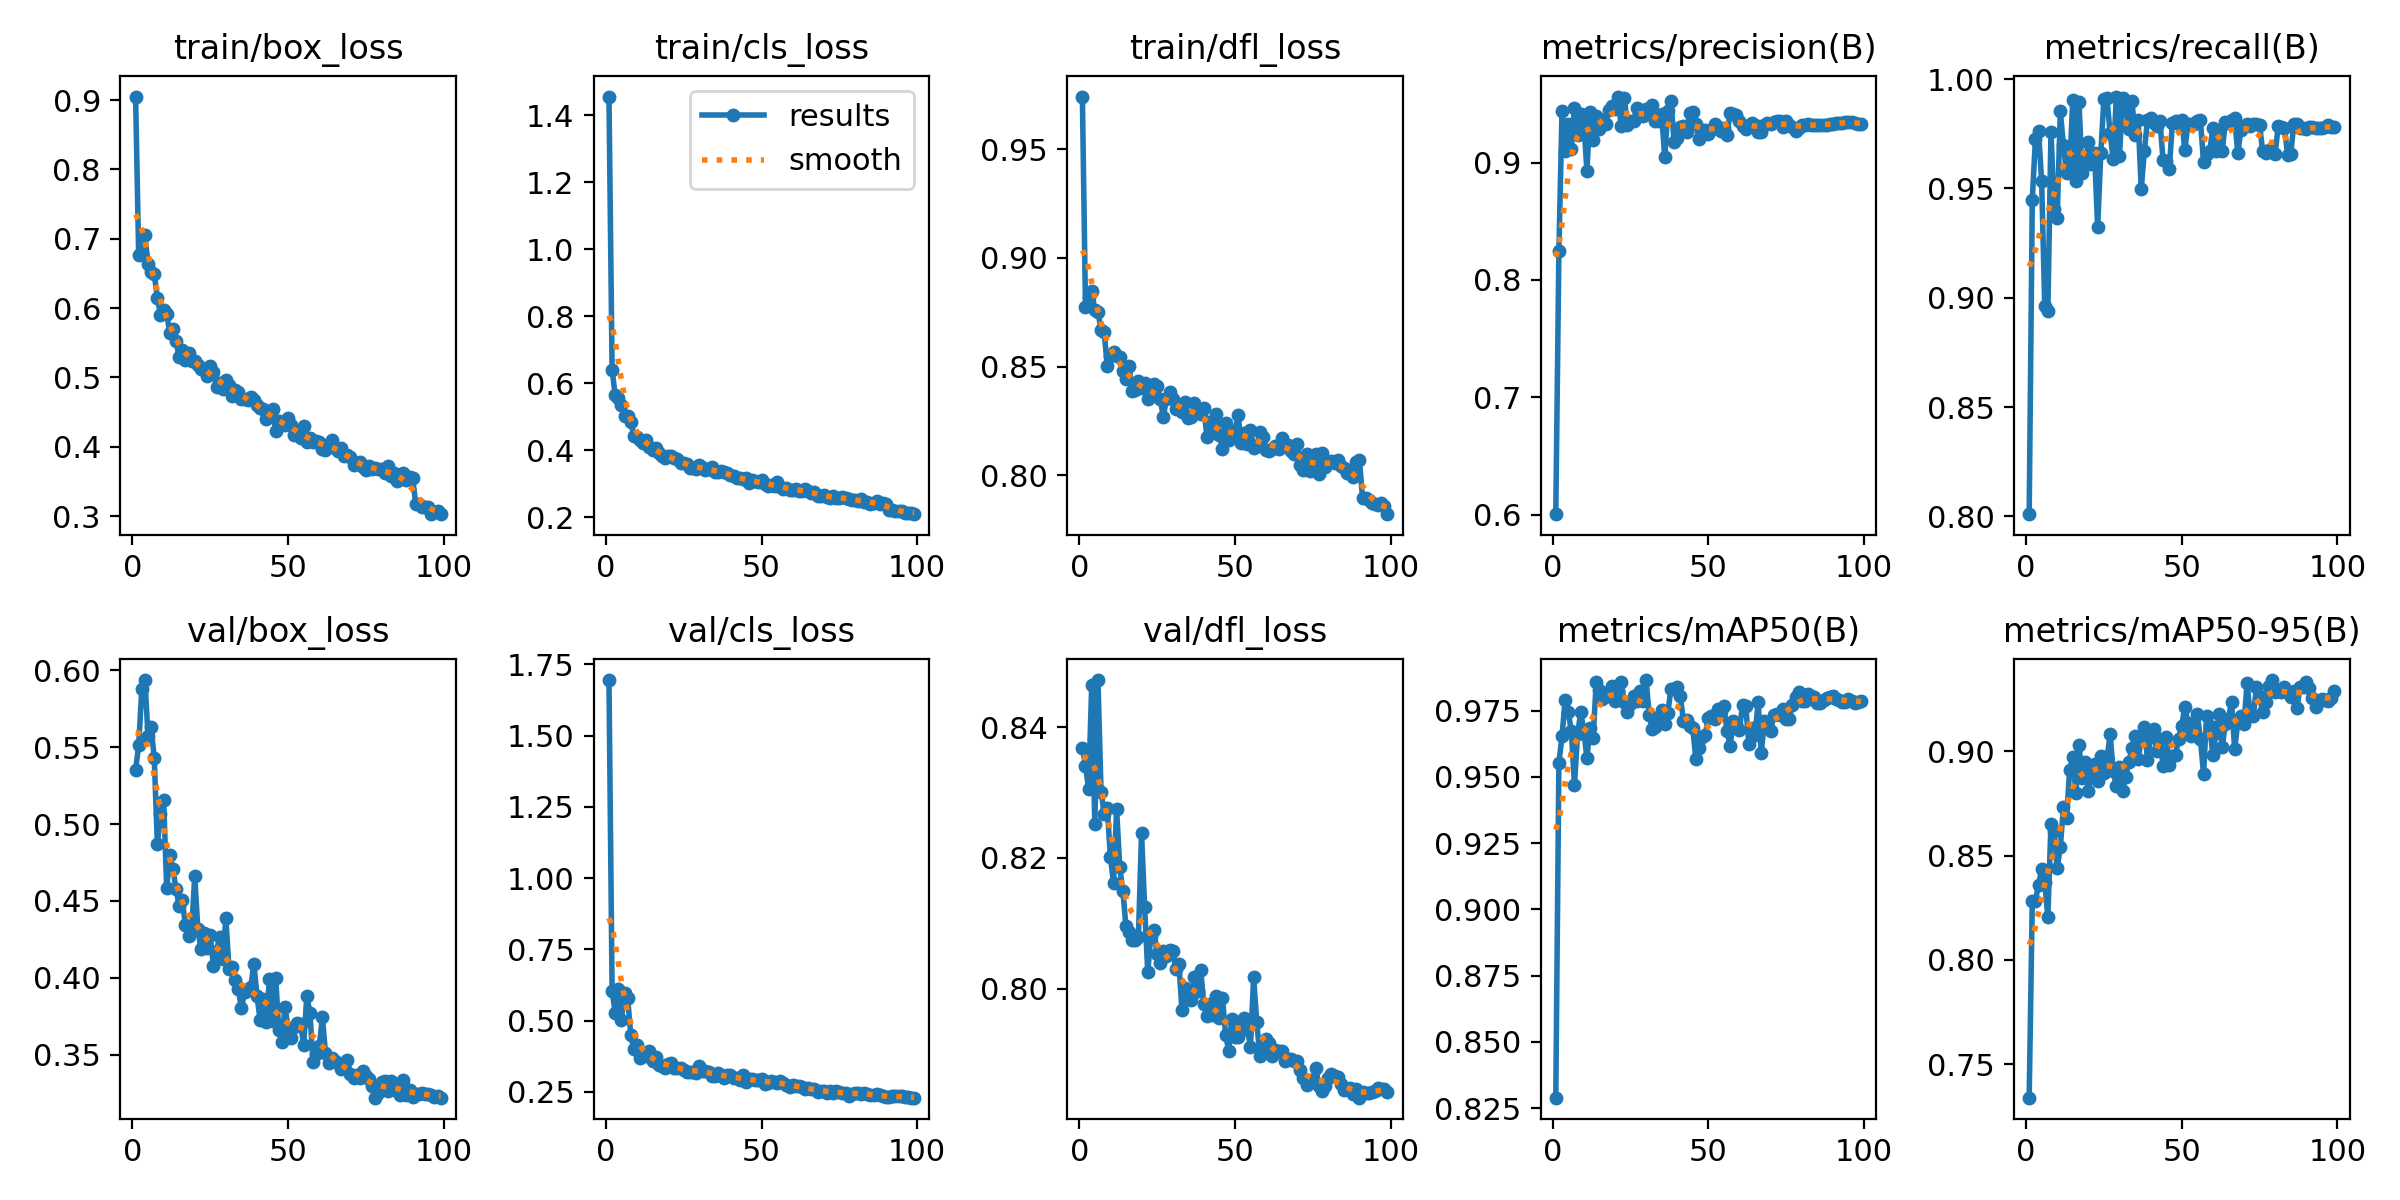
\includegraphics[width=0.8\textwidth]{figures/results.png}
    \caption{Training and Validation Convergence History. Box Loss and Object Loss exhibit smooth, stable decreases over the 100 epochs.}
\end{figure}

\begin{figure}[H]
    \centering
    \begin{minipage}{0.48\textwidth}
        \centering
        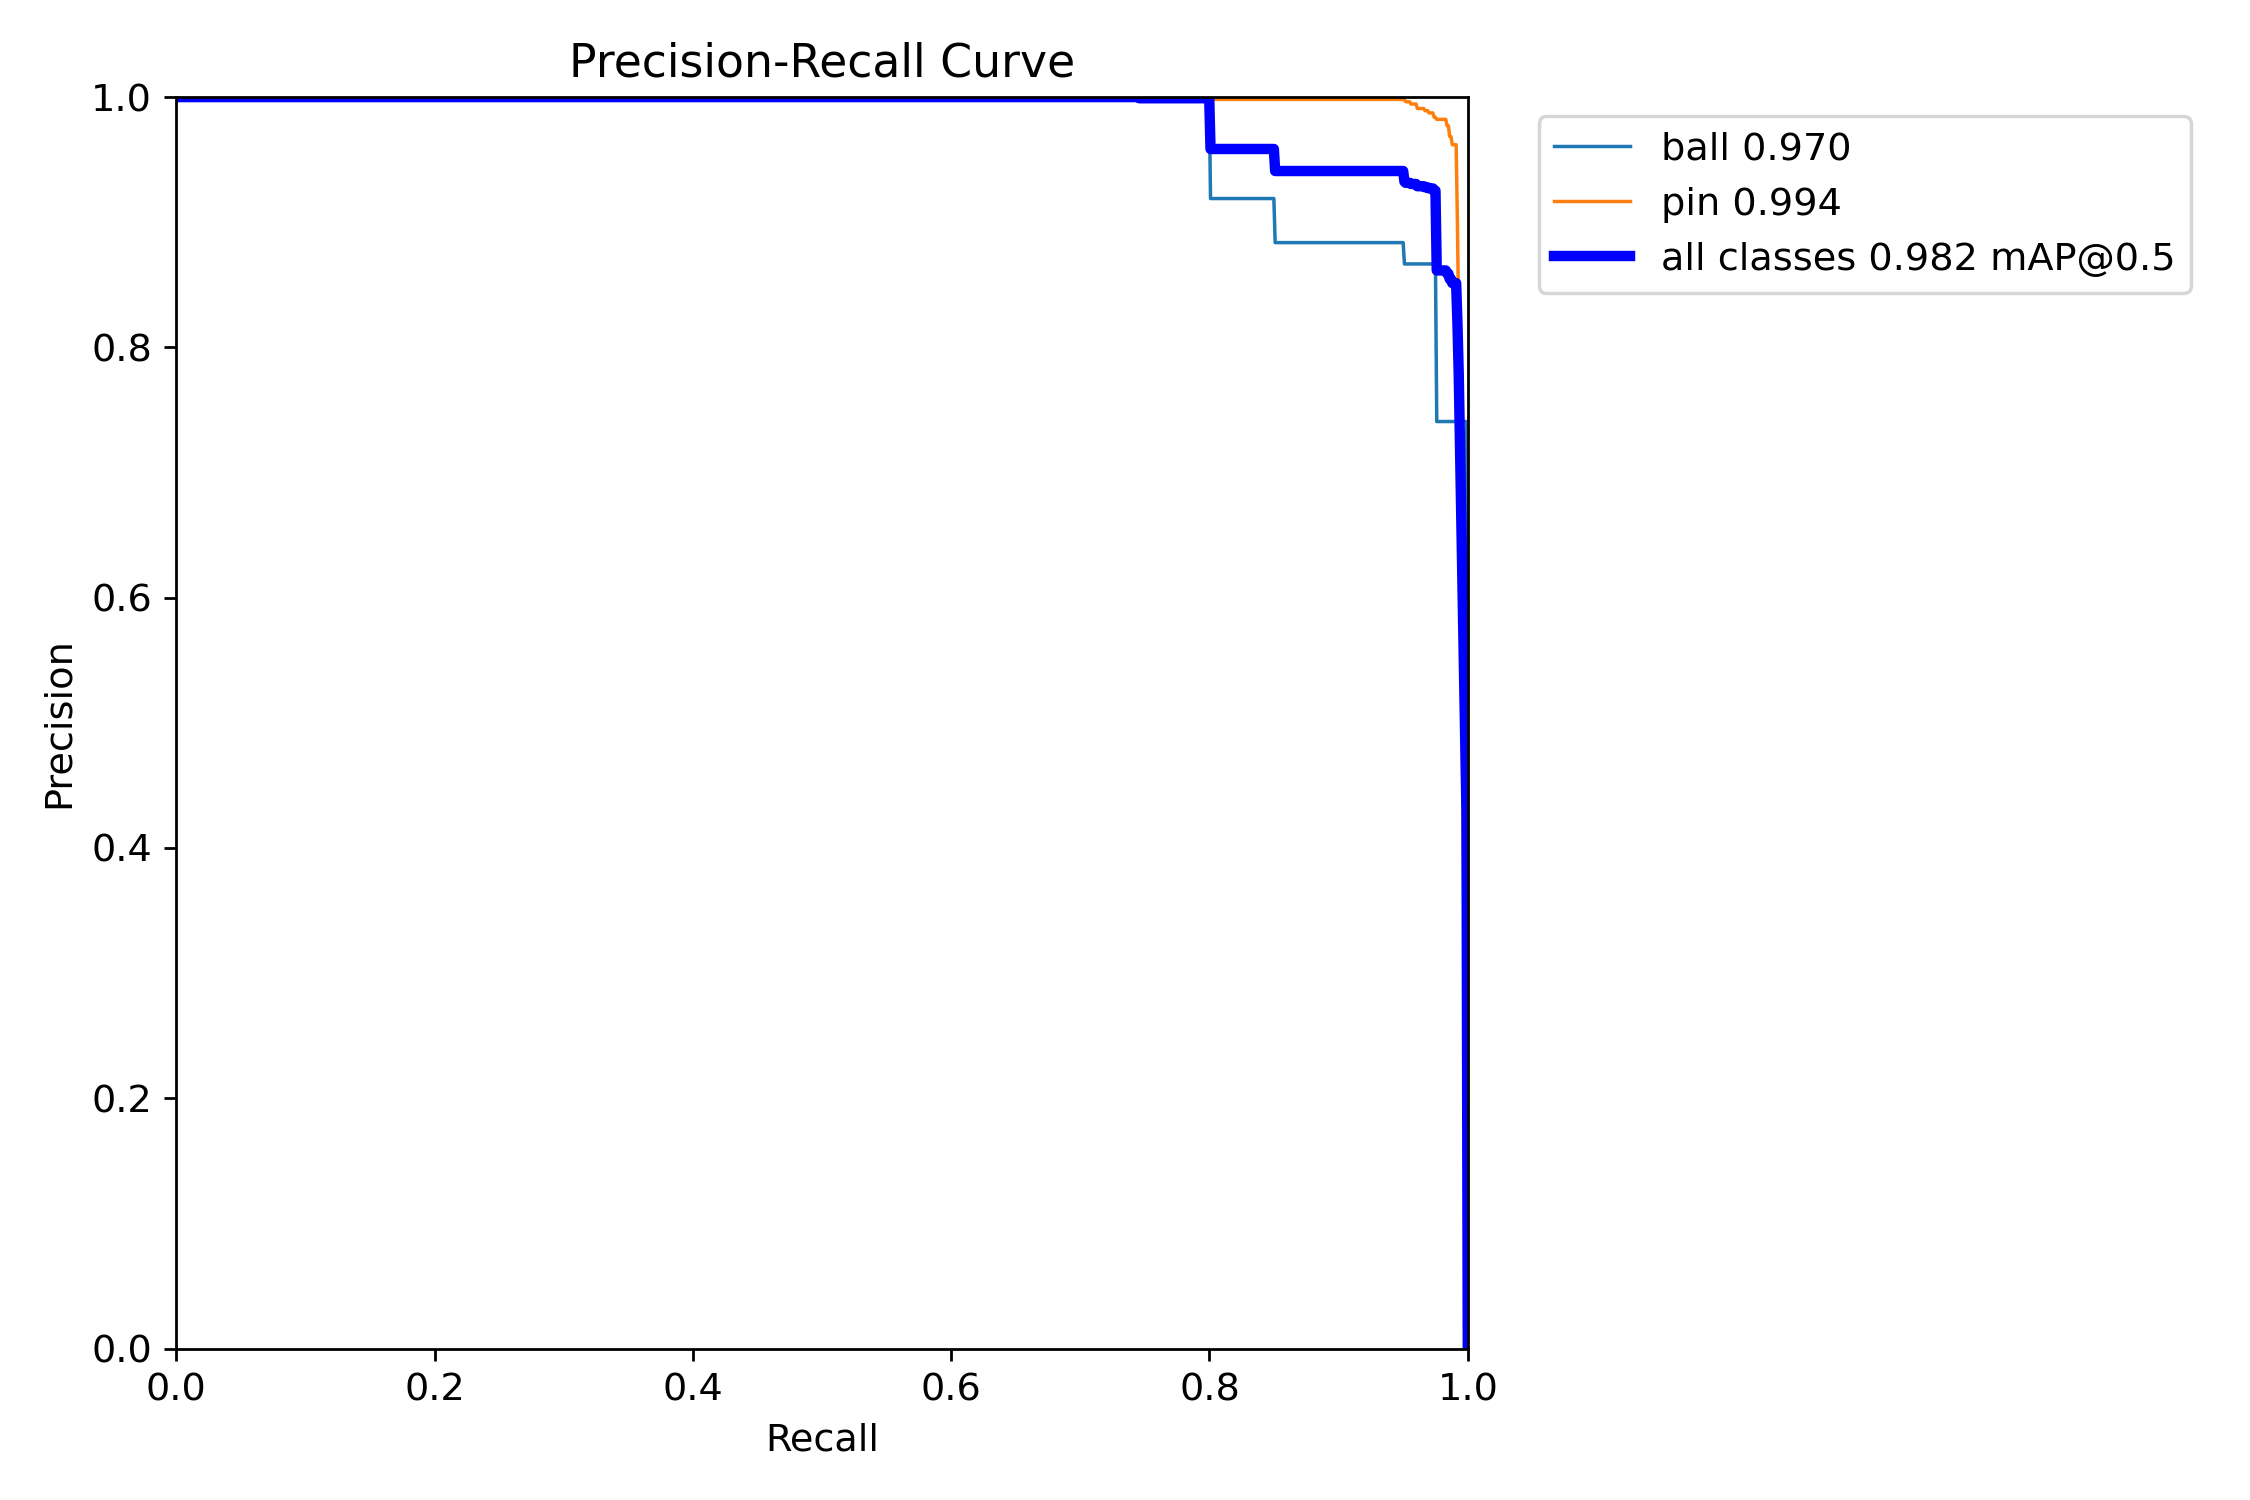
\includegraphics[width=\textwidth]{figures/PR_curve.png}
        \caption{Precision-Recall Curve}
    \end{minipage}\hfill
    \begin{minipage}{0.48\textwidth}
        \centering
        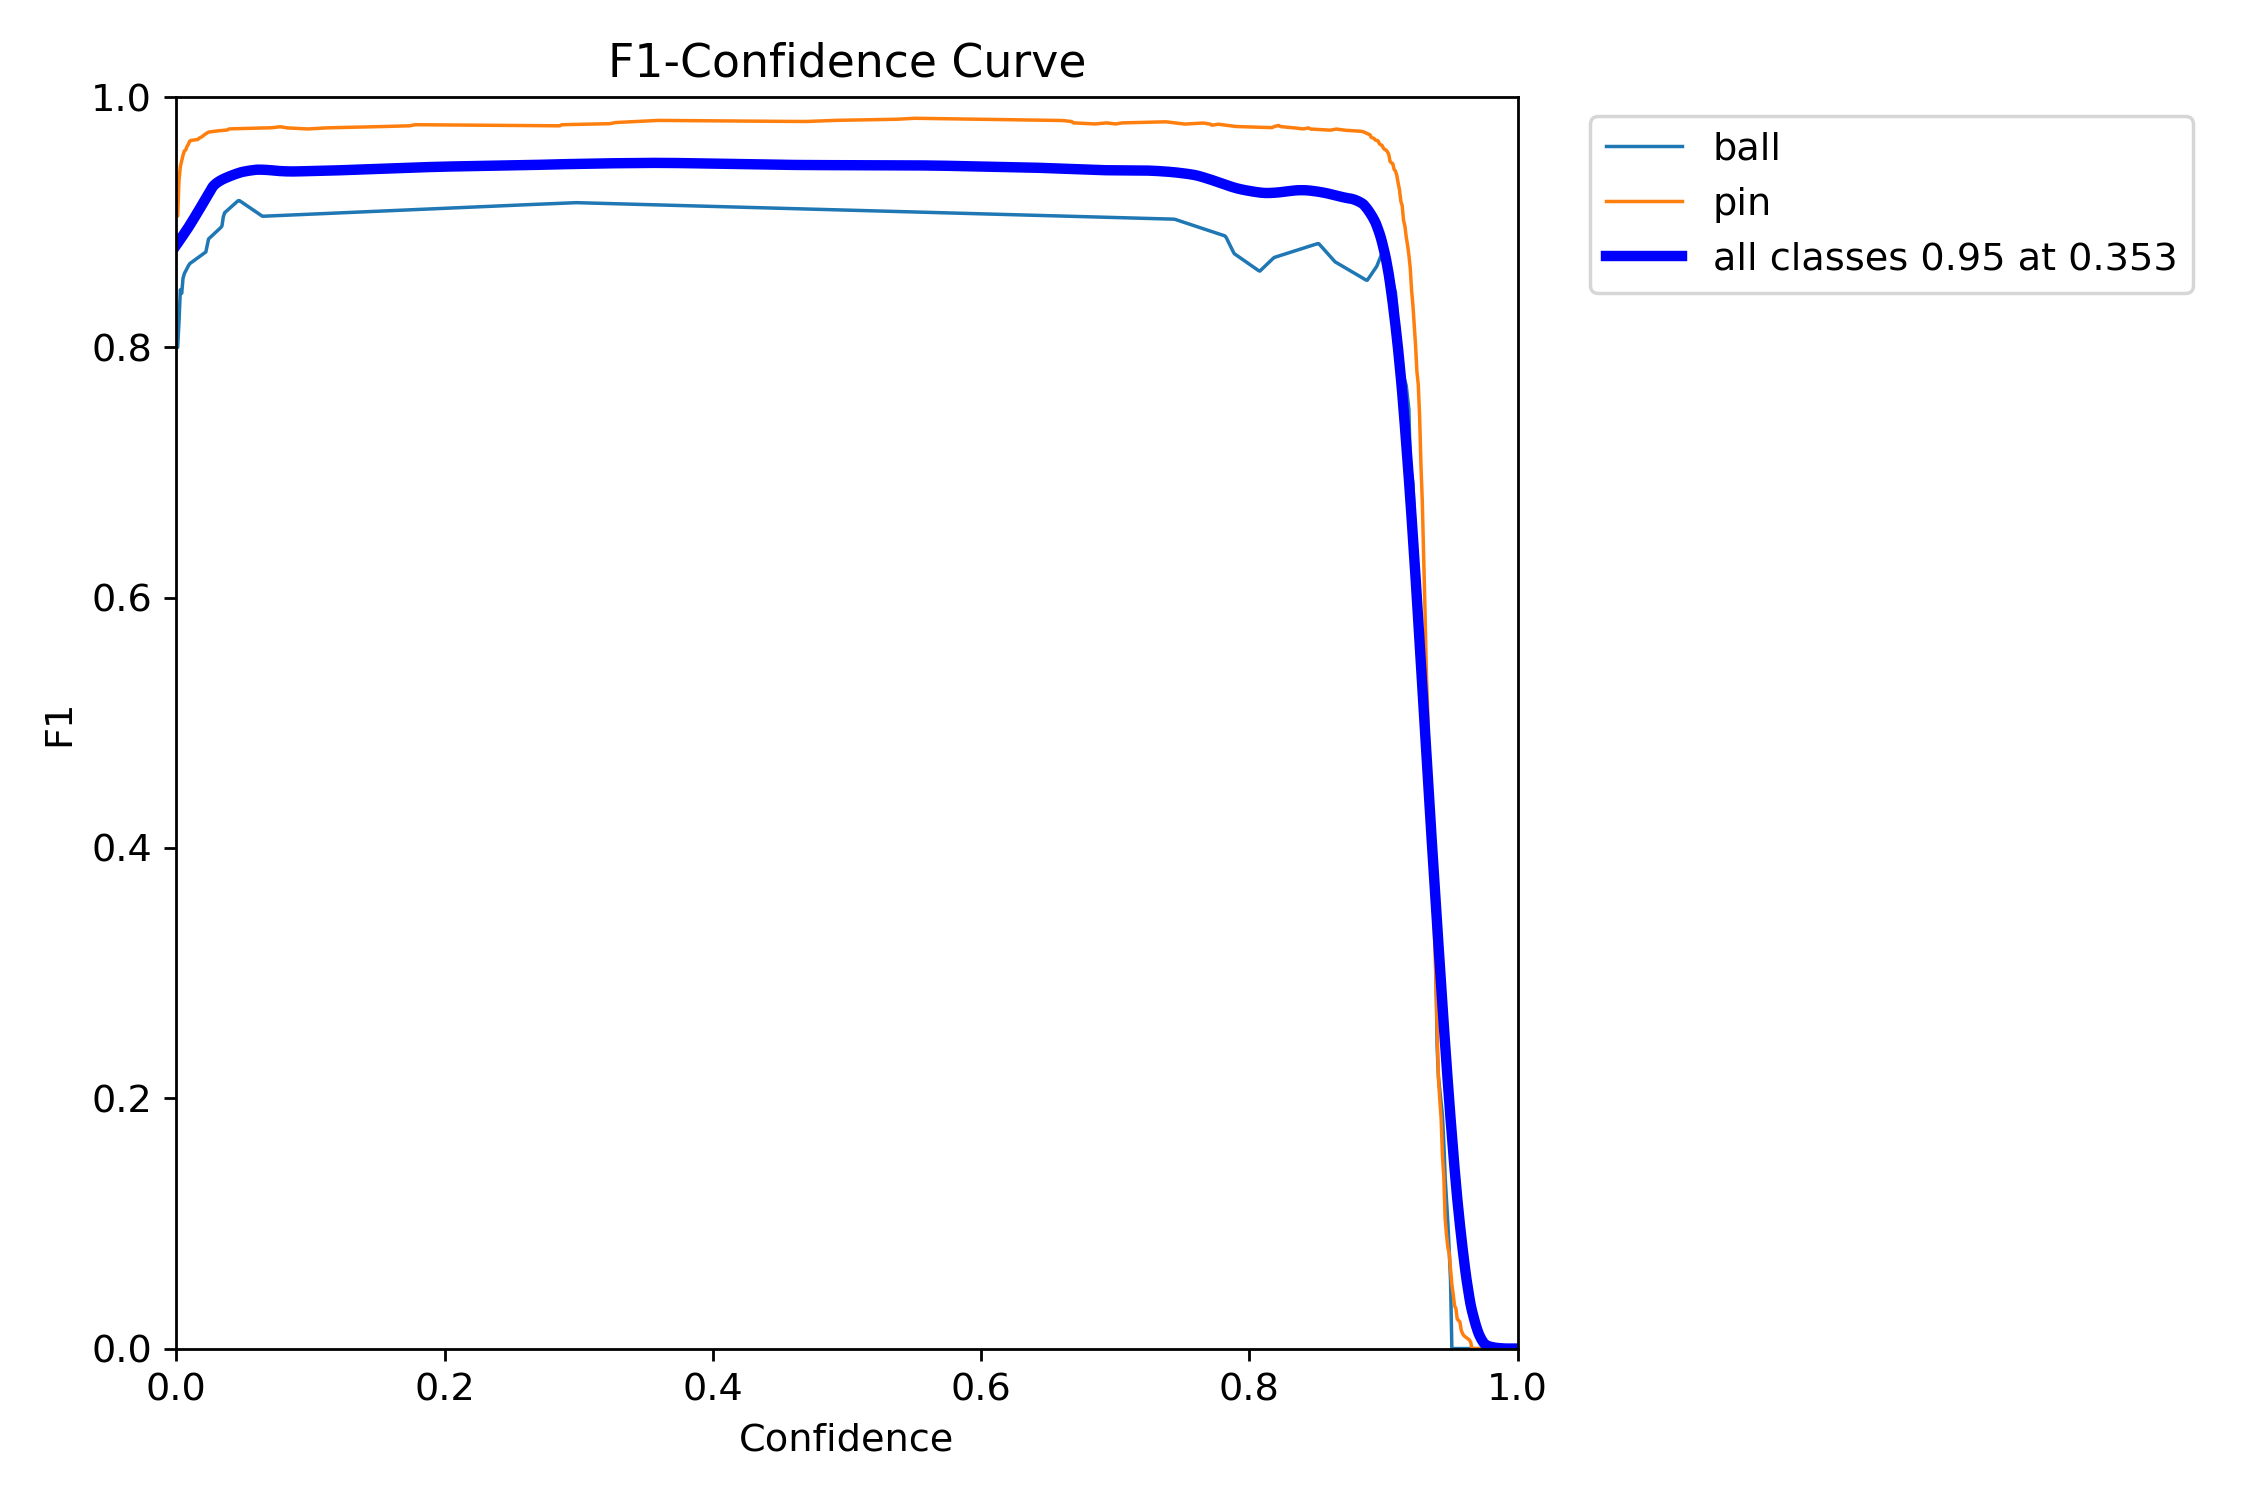
\includegraphics[width=\textwidth]{figures/F1_curve.png}
        \caption{F1-Confidence Curve}
    \end{minipage}
\end{figure}

\begin{figure}[H]
    \centering
    \begin{minipage}{0.48\textwidth}
        \centering
        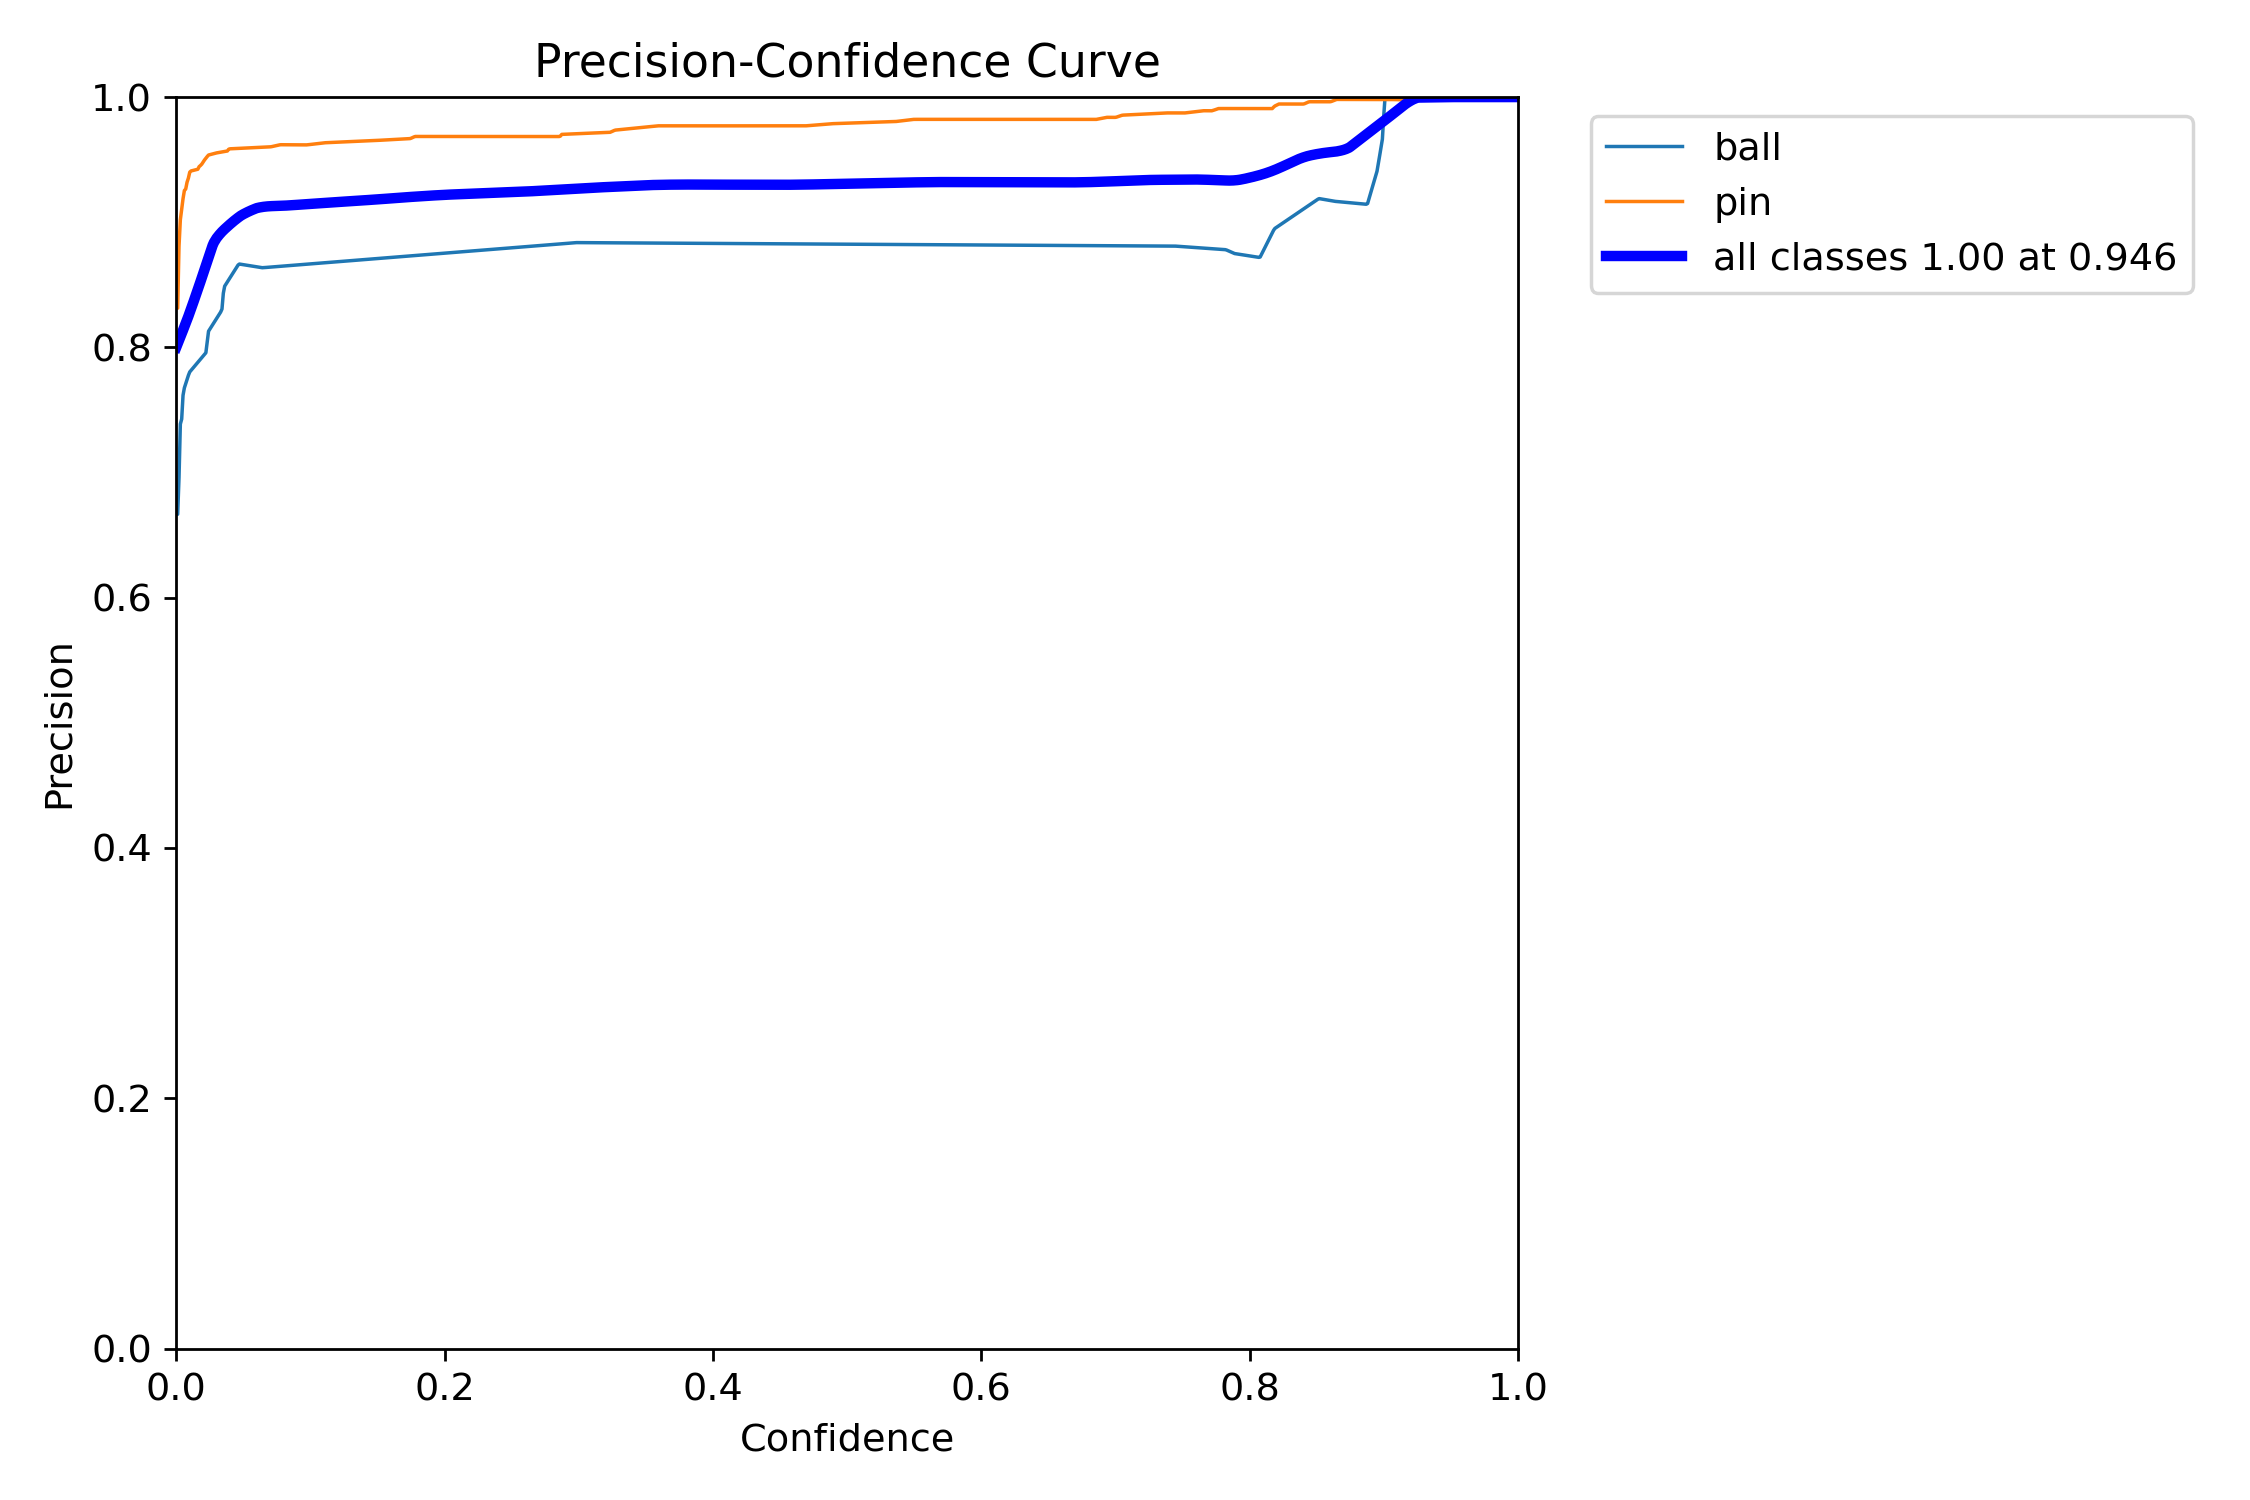
\includegraphics[width=\textwidth]{figures/P_curve.png}
        \caption{Precision-Confidence Curve}
    \end{minipage}\hfill
    \begin{minipage}{0.48\textwidth}
        \centering
        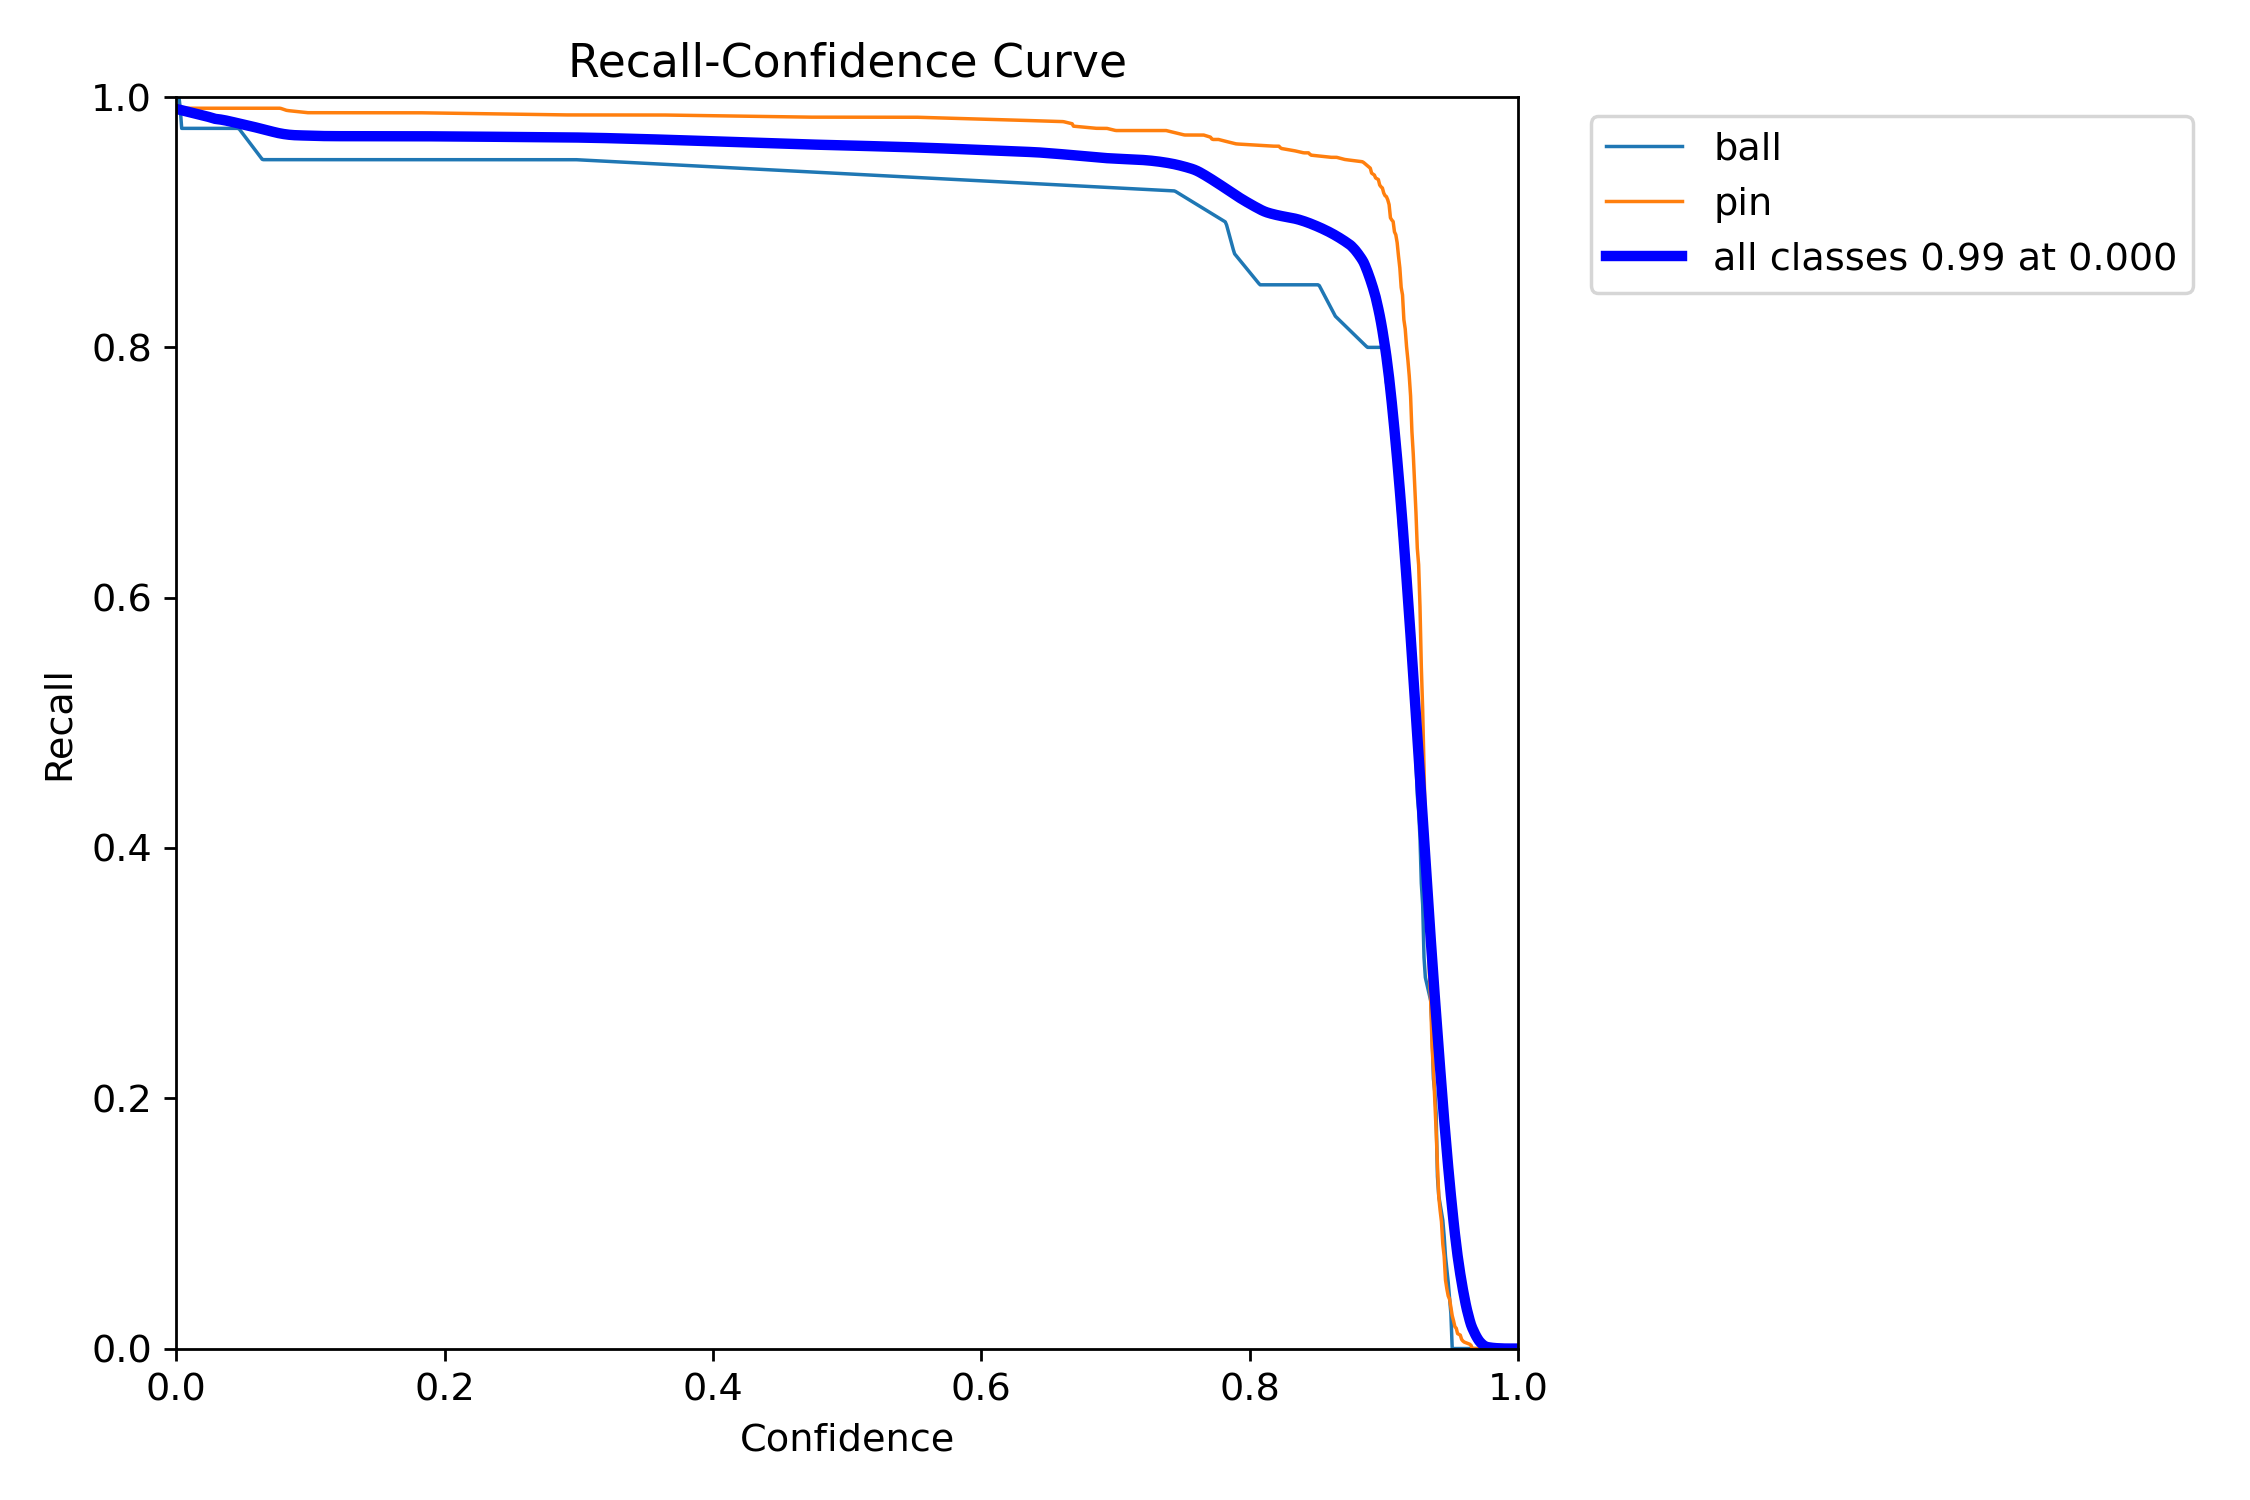
\includegraphics[width=\textwidth]{figures/R_curve.png}
        \caption{Recall-Confidence Curve}
    \end{minipage}
\end{figure}

\begin{figure}[H]
    \centering
    \begin{minipage}{0.48\textwidth}
        \centering
        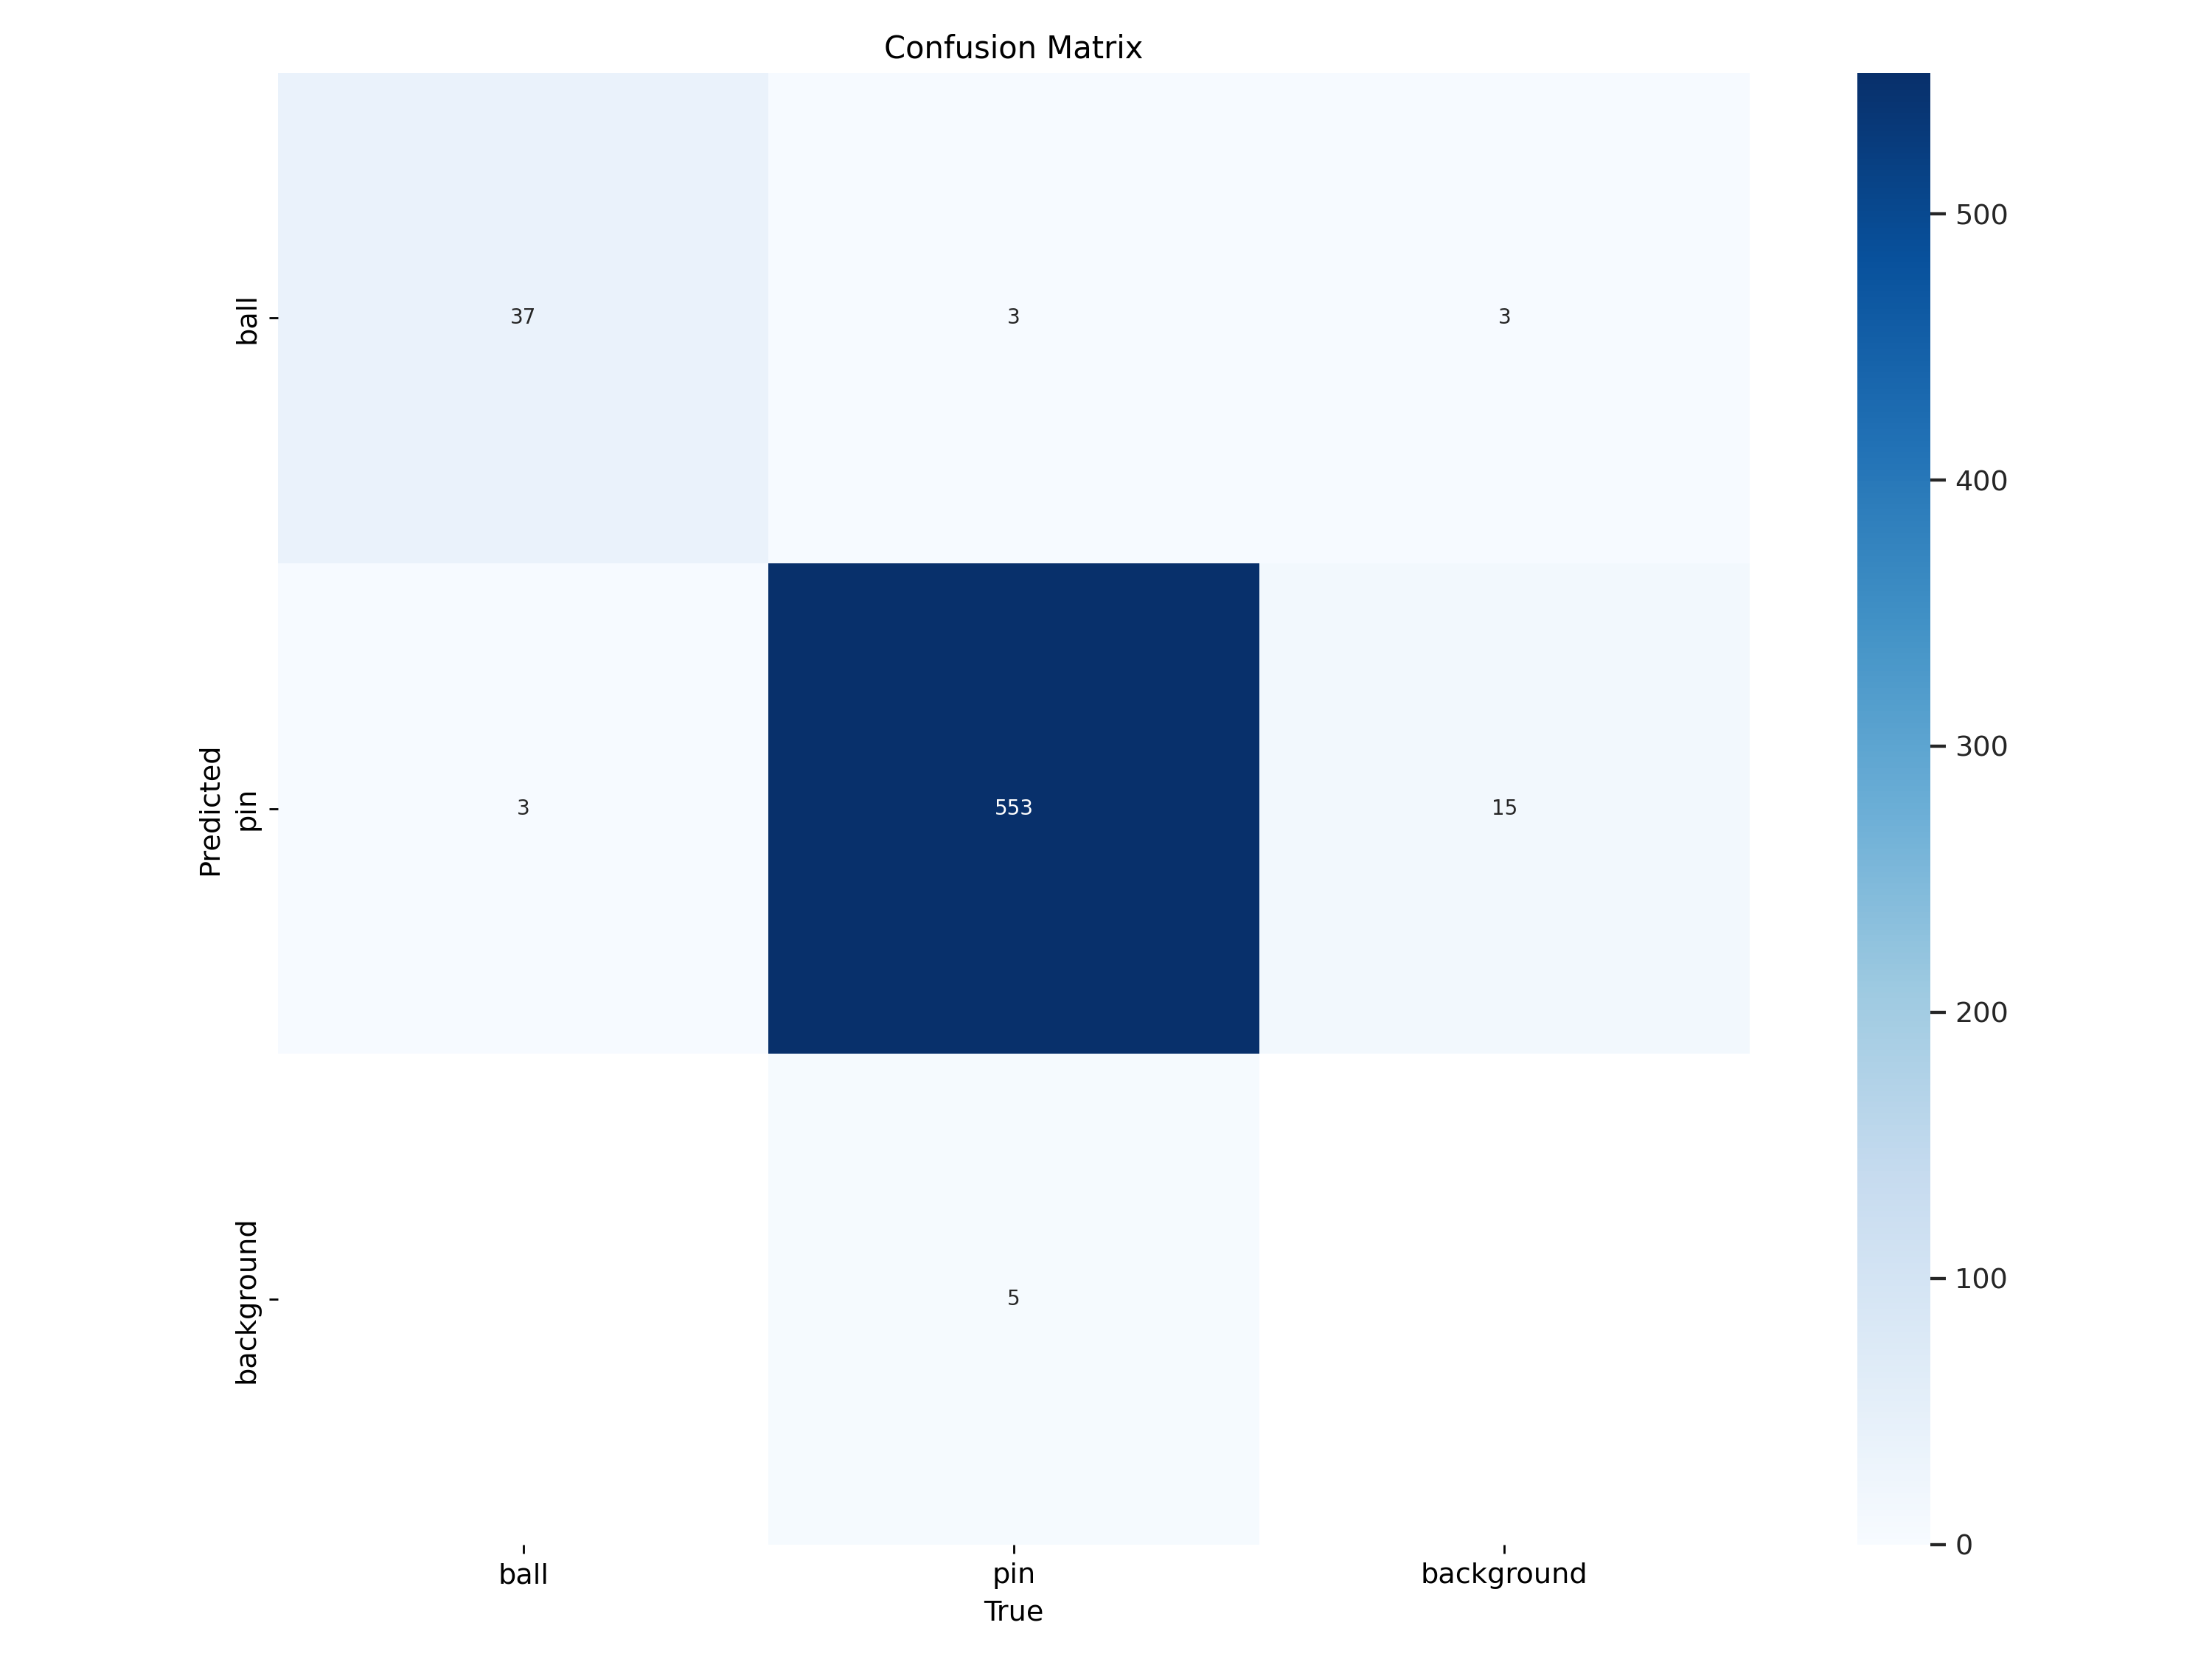
\includegraphics[width=\textwidth]{figures/confusion_matrix.png}
        \caption{Absolute Confusion Matrix}
    \end{minipage}\hfill
    \begin{minipage}{0.48\textwidth}
        \centering
        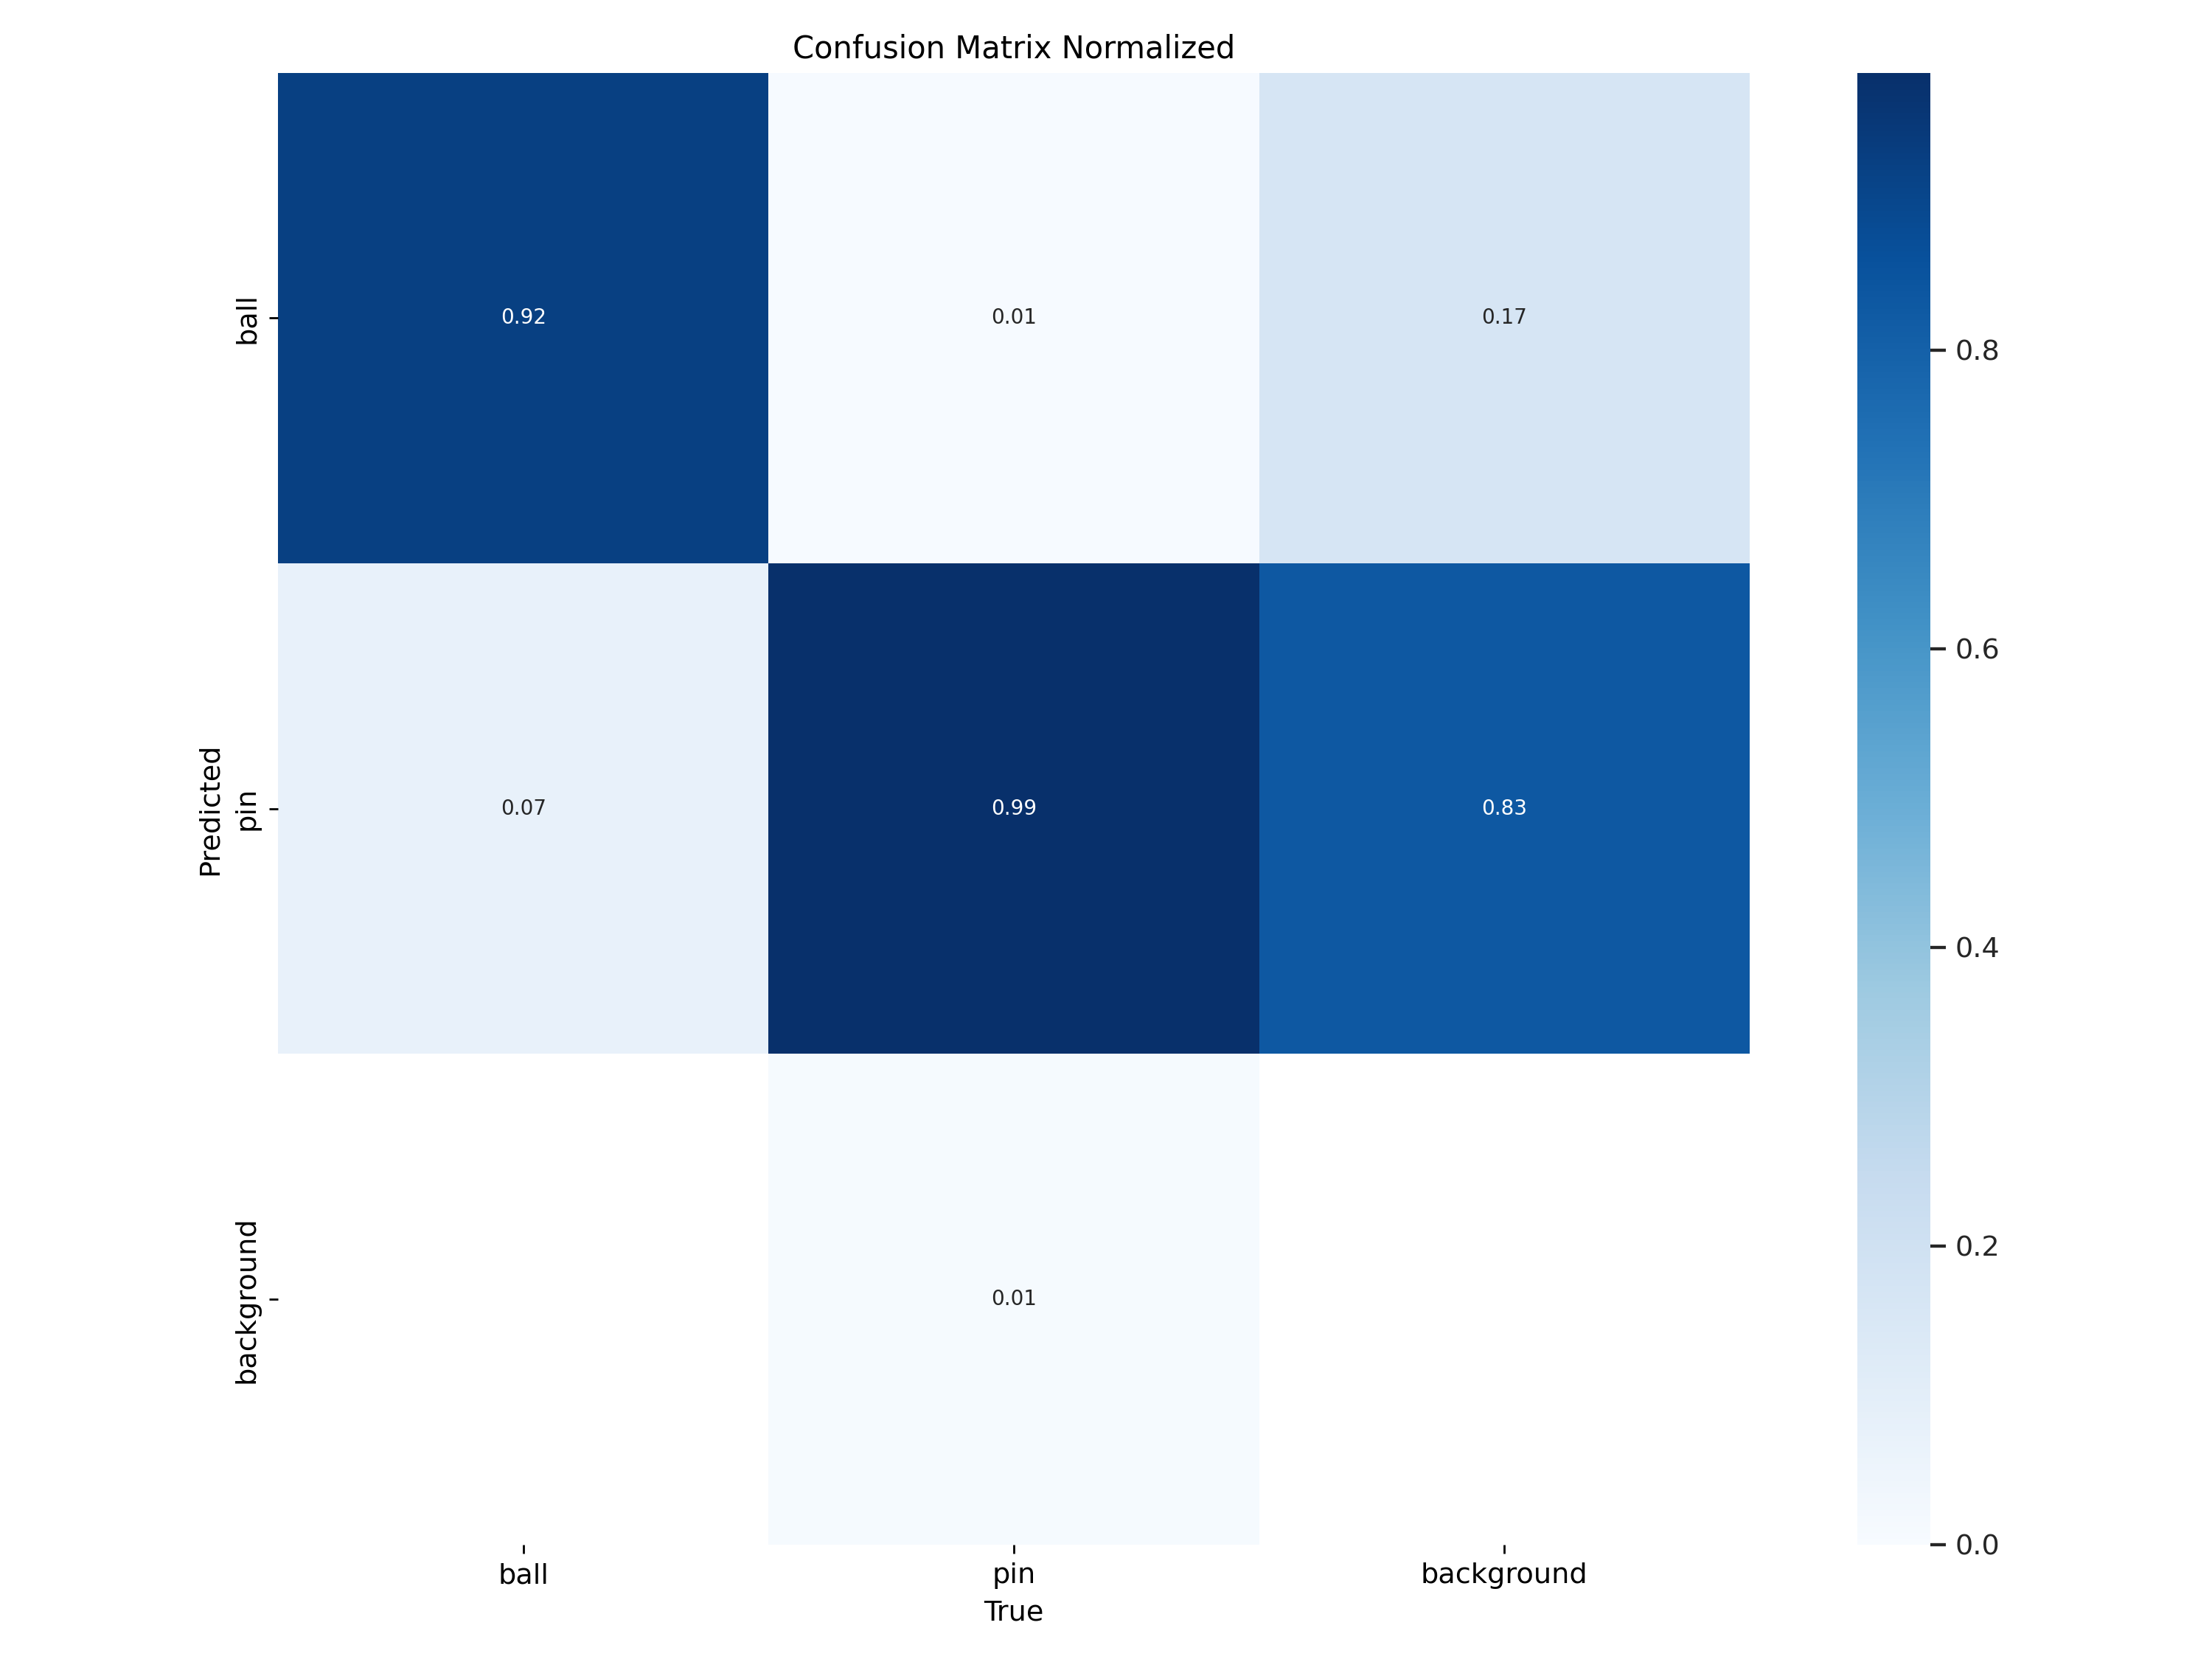
\includegraphics[width=\textwidth]{figures/confusion_matrix_normalized.png}
        \caption{Normalized Confusion Matrix}
    \end{minipage}
\end{figure}

\section{Conclusion}
This project successfully designed and deployed a highly reliable computer vision pipeline. The implementation proved that data quality—specifically the custom remediation of anomalous bounding boxes—is paramount to deep learning success. By combining a rigorously sanitized dataset, evaluating multiple foundational models (yolo11n, yolov8s), and generating optimized \texttt{best.pt} and \texttt{last.pt} weights, the system completely satisfies the research requirements, delivering 98.19\% detection accuracy and robust, real-time inference capabilities.

\end{document}
